\documentclass{article}

% Informations

%Modules 
\usepackage[greek,english,french]{babel}
\usepackage{graphicx}                       % Gestion des images
\usepackage{caption}                        % Gestion des titres
\usepackage{appendix}                       % Gestion de l'annexe
\usepackage[utf8]{inputenc}                 % Encodage du texte
\usepackage{multicol}                       % Gestion des multi-colonnes des tableaux
\usepackage{multirow}
\usepackage{booktabs}                       % Importation des traits horizontaux des tableaux
\usepackage{siunitx}                        % Gestion des unités
\usepackage{mwe,lipsum}                     % Modules de Minimal Working Examples
\usepackage{amsmath,amssymb,amsbsy}         % Ajout d'options dans le mode 'math'
\usepackage{todonotes}                      % Ajout des notes en marge
\usepackage{mathtools}                      % Autres outils pour le mode 'math'
\usepackage[a4paper]{geometry}                       % Options de mise en page
\usepackage{listings}
\usepackage{color,xcolor}
\usepackage{csquotes}
\usepackage{textcomp}
\usepackage{fancyhdr}
\usepackage{lmodern}
\usepackage[T1]{fontenc}
\usepackage{lato}
\usepackage{titling}
\usepackage{datetime}
\usepackage[version=4]{mhchem}
\usepackage{enumitem}
\usepackage{pdfpages}
\usepackage{stmaryrd}
\usepackage{hyphenat}
\usepackage{tablefootnote}
\usepackage{cases}
\usepackage{bbm}
\usepackage{empheq}
\usepackage{gensymb}
\usepackage{pythonhighlight}
\usepackage{tfrupee}

% Police d'écriture
\renewcommand\familydefault{\sfdefault}

% Définition de couleurs
\definecolor{Bleu_ENSPS}{RGB}{0,119,139}
\usepackage[colorlinks=true,allcolors=Bleu_ENSPS]{hyperref} 

% Options de format pour les unités (SIUnitX package)
\sisetup{
    detect-all,
    locale                  = FR,
    sticky-per,
    inter-unit-product      = {.},
    per-mode                = reciprocal-positive-first,
    % scientific-notation     = true,
}

\DeclareSIUnit\octet{o}
\DeclareSIUnit\year{an}
\DeclareSIUnit\watthour{Wh}
\DeclareSIUnit\degreehour{\degree Ch}
\DeclareSIUnit\degreeday{\degree Cday}
\DeclareSIUnit\euro{€}
\DeclareSIUnit\tCOeq{t\ce{CO_2}éq}
\DeclareSIUnit\inhab{hab}
\DeclareSIUnit\indianrupee{\rupee}

%Options de largeur de marges, verticales et horizontales
\geometry{hmargin=3cm,vmargin=2cm}
\setlength{\parindent}{7mm}

% Mise en page
\pagestyle{fancy}
\setlength{\headheight}{14pt}
\renewcommand\headrulewidth{0.5pt}
\renewcommand\footrulewidth{0.5pt}
\fancyhead[C]{\thedate}
\fancyhead[R]{}%\rightmark
\fancyhead[L]{}

% Bibliographie
% \usepackage[style=authoryear]{biblatex}
\usepackage[style=authoryear]{biblatex}
\DefineBibliographyExtras{french}{\restorecommand\mkbibnamefamily}

\AtEveryBibitem{%
  \clearlist{language}%
  \clearlist{urldate}
  % \clearlist{url}
  \clearfield{month}
  \clearfield{day}
  \clearfield{note}
}
% \DeclareFieldFormat{url}{}
\DeclareFieldFormat{urldate}{}

\DeclareFieldFormat{journaltitle}{\textit{#1}}
\DeclareFieldFormat{title}{#1}

\setlength\bibitemsep{\itemsep}
% \AtEveryCite{\color{Bleu_ENSPS}}

\addbibresource{/home/amounier/Documents/Bibliographie/bibliographie_bib.bib}

% All name in hyperlink (cite biblatex)
\makeatletter
\let\abx@macro@citeOrig\abx@macro@cite
\renewbibmacro{cite}{%
   \bibhyperref{%
   \let\bibhyperref\relax\relax%
   \abx@macro@citeOrig%
   }%
}
\let\abx@macro@textciteOrig\abx@macro@textcite
\renewbibmacro{textcite}{%
   \bibhyperref{%
   \let\bibhyperref\relax\relax%
   \abx@macro@textciteOrig%
   }%
}%
\makeatother

% Passage des mots table et figure dans les lien hypertextes
\makeatletter
\renewcommand\p@table{Table~\@ }
\renewcommand\p@figure{Figure~\@ }
\makeatother

% Styles équations
%\numberwithin{equation}{section}

%Autres commandes
% \newcommand{\CO}{\ce{CO_2}}
\newcommand{\mail}[1]{\href{mailto:#1}{#1}}

% Titre ---------------------------------------
\date{\today}
\title{Taux d'équipement en climatisation en Inde}
\author{\href{mailto:andre.mounier@enpc.fr}{André Mounier}}

\begin{document}

{\huge \noindent \thetitle}

\vspace{3mm}
{\Large \noindent \theauthor}

% Contenu -------------------------------------

\vspace{1cm}

\section{Description}

Le but est de caractériser une fonction permettant le relier le climat et le niveau de vie au taux d'équipement en climatisation. Le climat est exprimé à travers les degrés-jours de refroidissement (CDD) et le niveau de vie en PIB par habitant. Une fois cette fonction caractérisée, elle peut être utilisée pour réaliser des projections de taux d'équipement dans le futur, en projetant des valeurs de CDD et de PIB par habitant. \\

L'ensemble des données, résultats et codes sont disponibles sur un dépôt distant git : \url{https://github.com/amounier/ac_india/}. Ces codes permettent de tracer les différentes cartes, formatter les données et réaliser les calculs des paramètres de modélisation. 

\section{Modélisation}

\subsection{Données}

\noindent
Les données disponibles et nécessaires pour la modélisation, à l'échelle des états, sont :
\begin{itemize}
   \item Le nombre de climatiseurs (en unité) (\cite{mspi_nss_2023});
   \item Le nombre d'habitants (--);
   \item Le nombre de logements (--);
   \item Le PIB (--);
   \item Les \textit{Cooling degree-days} (CDD) (\cite{iea_weather_2023}).
\end{itemize}

Nous nous basons sur les données de 2021. Les cartes de taux d'équipement, de PIB par habitant et de CDD sont décrites \ref{fig:gdp_ac} et \ref{fig:cdd1826}.

\begin{figure}[ht]
   \centering
   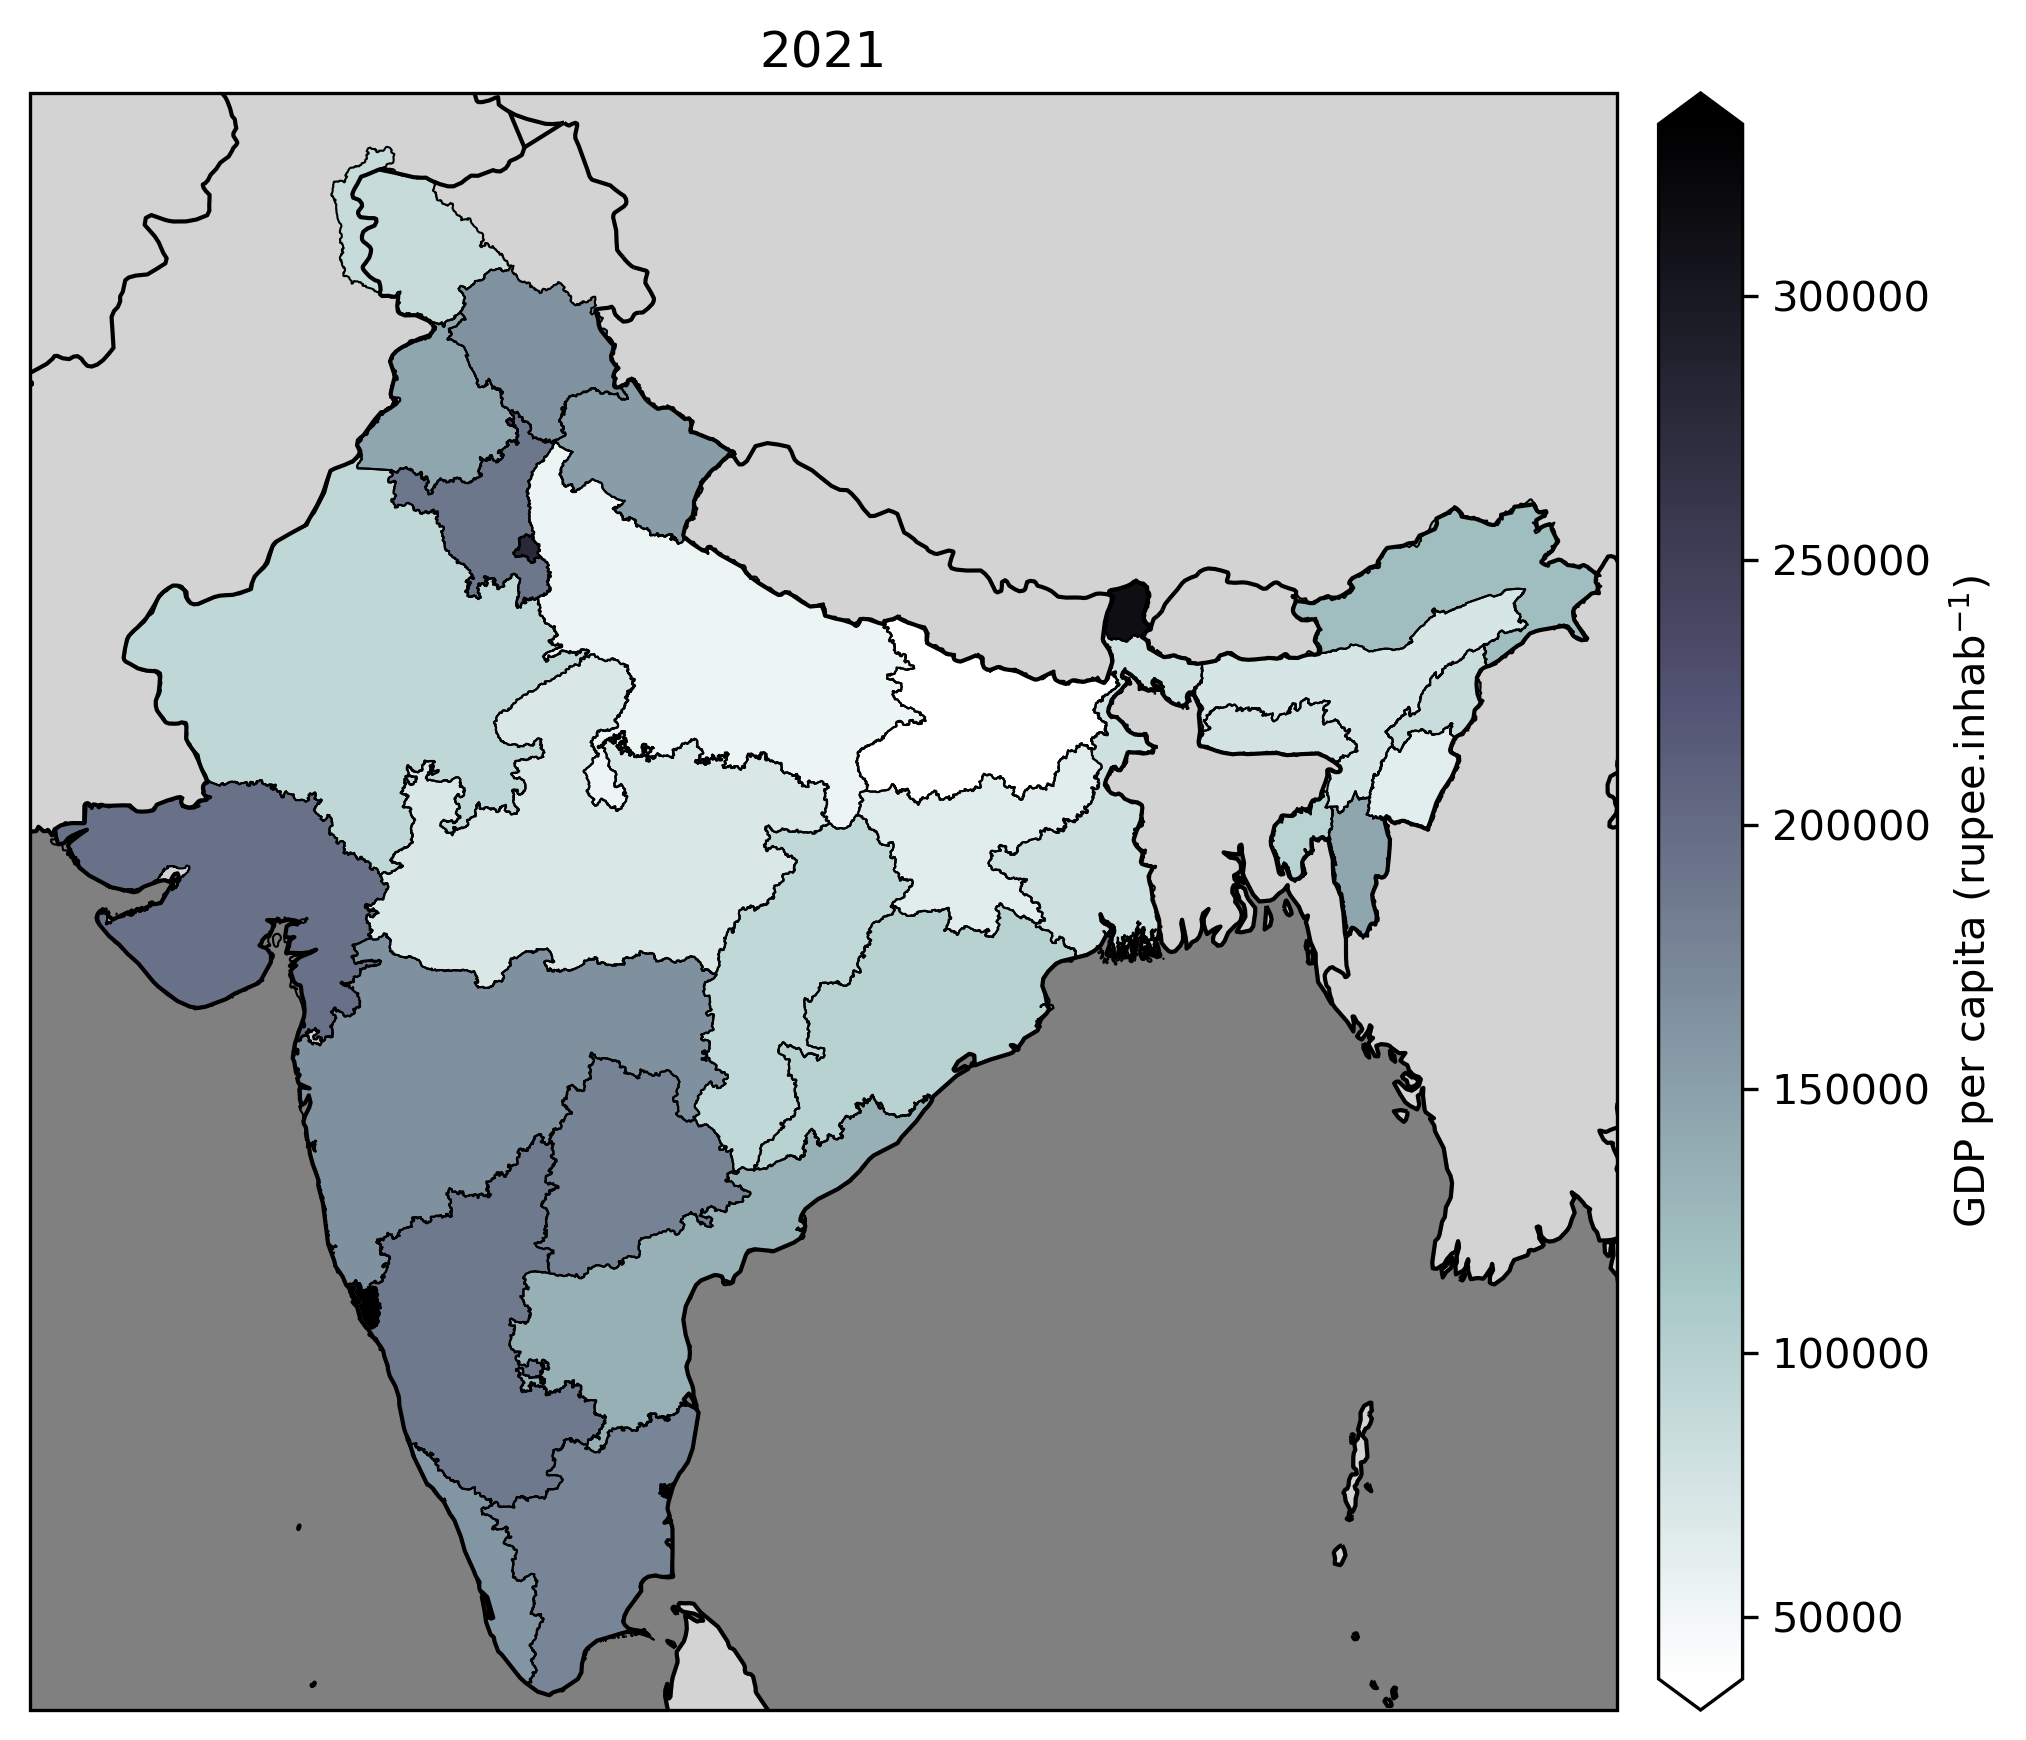
\includegraphics[width=0.49\columnwidth]{figures/20260403_gdp_per_capita_2021.png}
   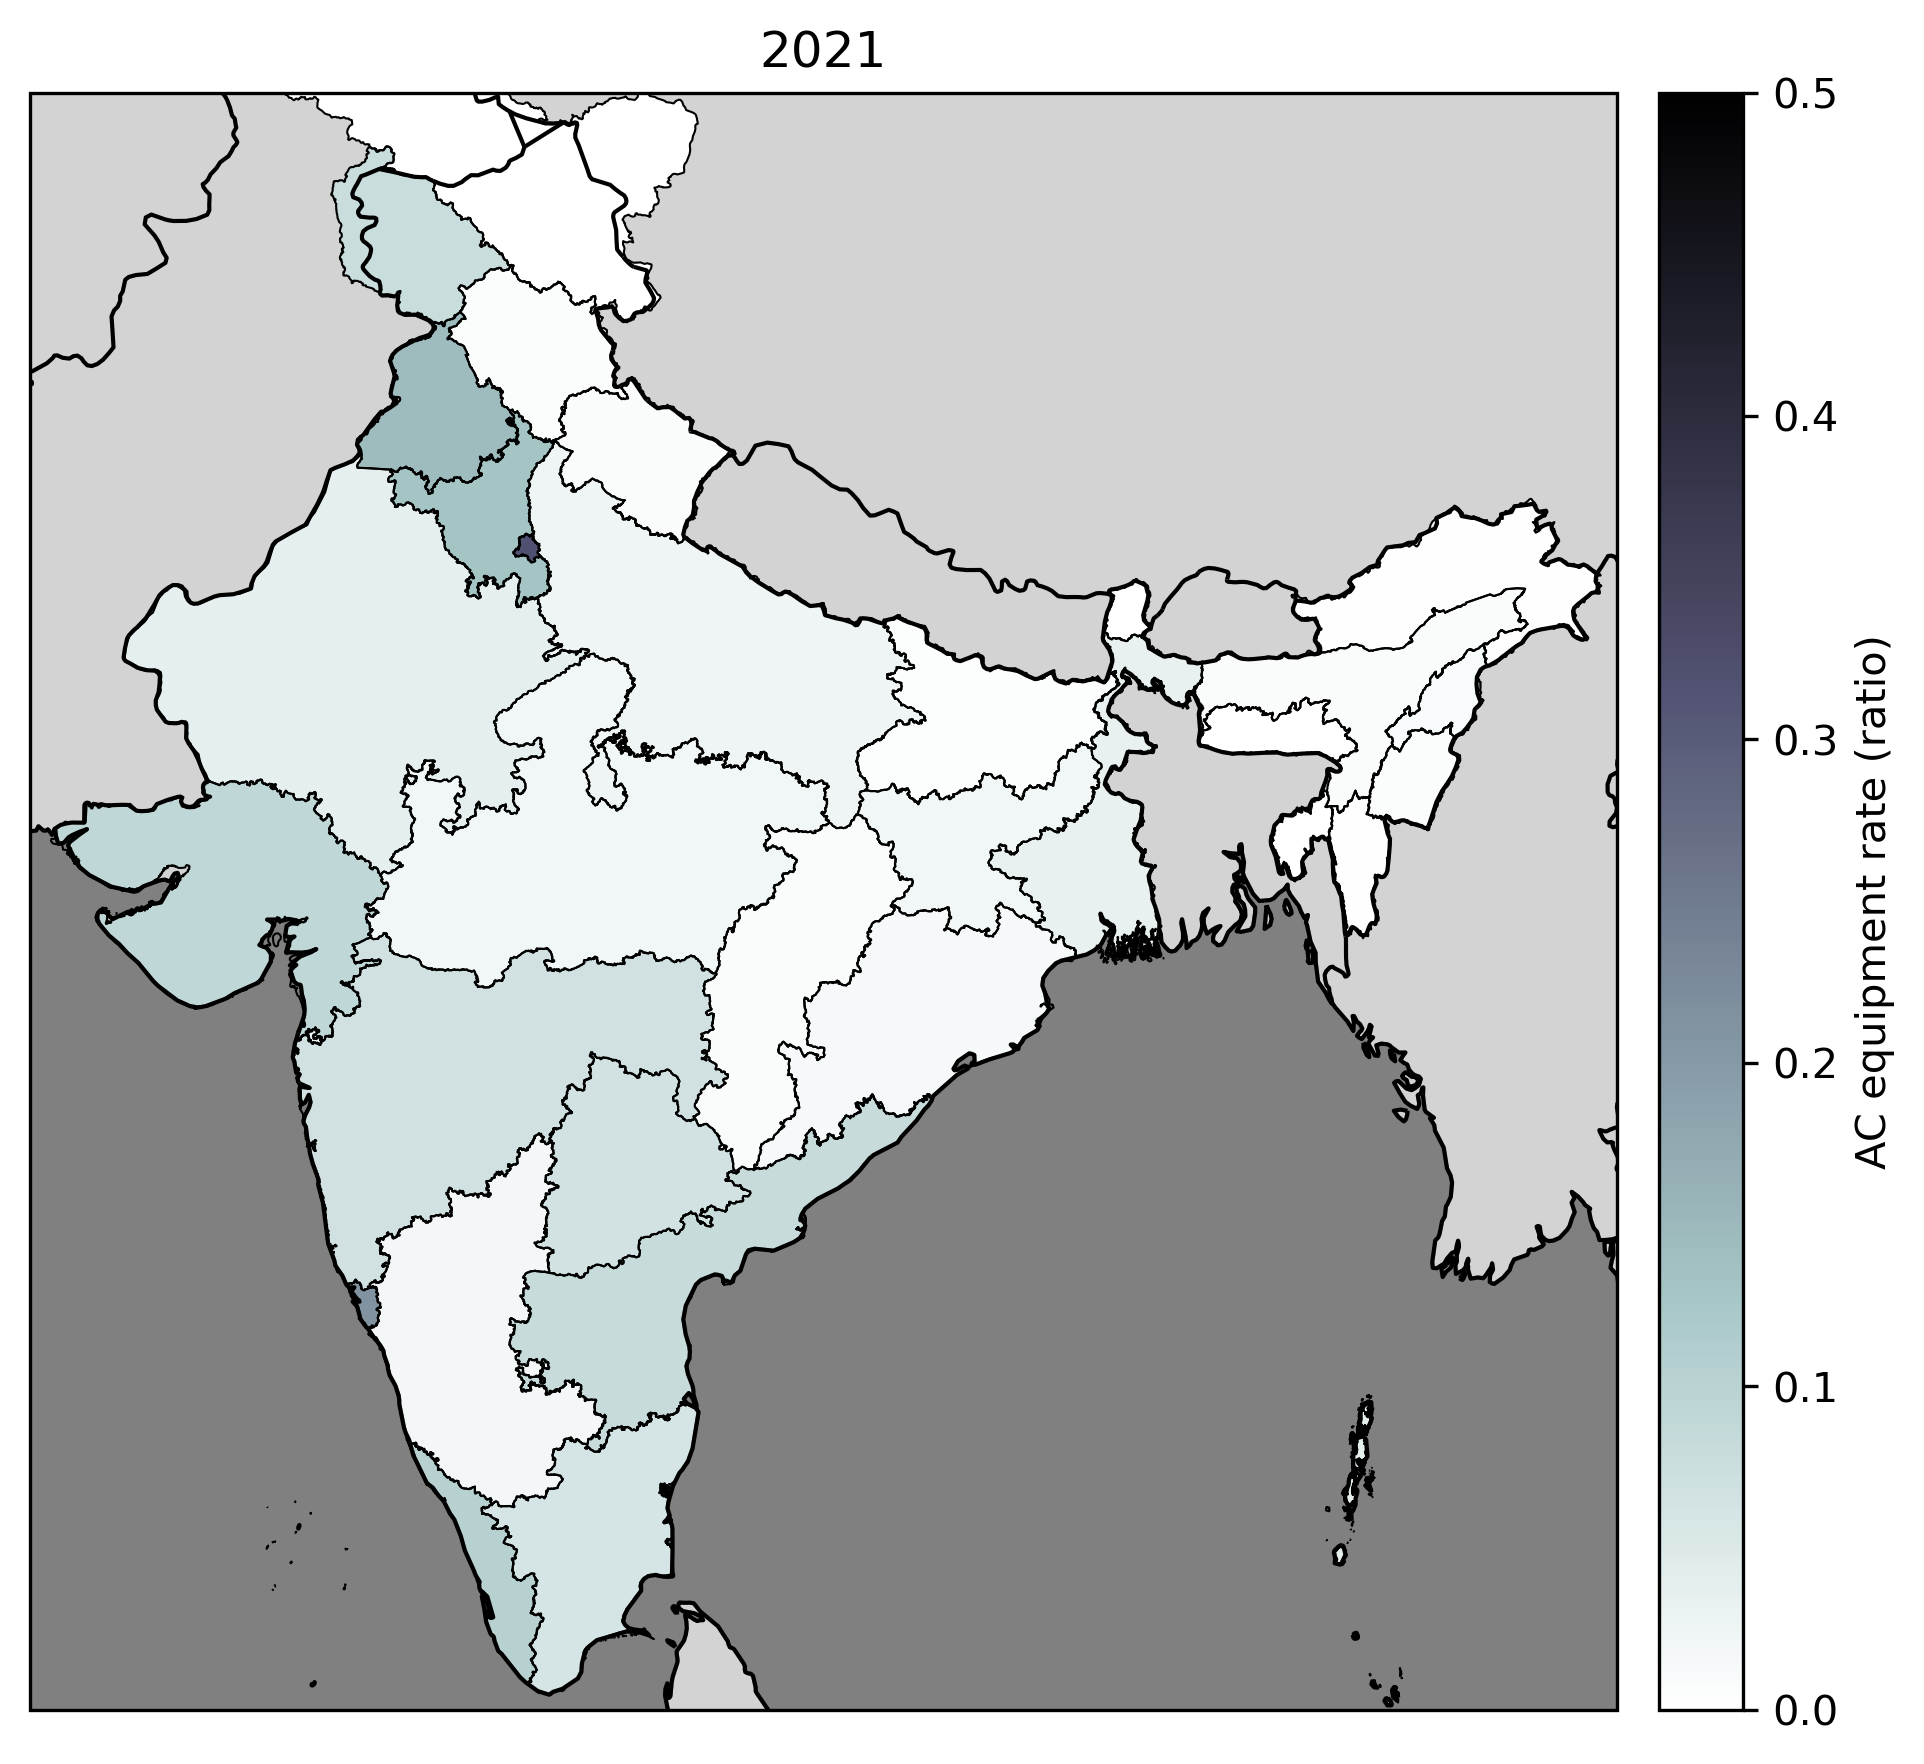
\includegraphics[width=0.46\columnwidth]{figures/20260404_ac_rate_2021.png}
   \caption{\label{fig:gdp_ac} Carte du PIB par habitant et des taux d'équipement en climatisation par état.}
\end{figure}

\subsection{Modèles}

La modélisation utilisée dans la littérature pour relier le taux d'équipement $\tau$ de climatisation aux variables de climat ($\mathrm{CDD}$) et de revenu ($\mathrm{GDP}$) resulte de la mutliplication d'une fonction exponentielle décroissante ($\mathrm{E}$) et d'une sigmoïde ($\mathrm{S}$) (\cite{mcneil_future_2008,isaac_modeling_2009,akpinar-ferrand_modeling_2010}). Ce modèle de base est alors noté $\mathrm{E-S}$ est s'écrit \eqref{eq:es}.

\begin{equation}
   \label{eq:es}
   \tau(\mathrm{CDD},\mathrm{GDP}) = \underbrace{\left(\vphantom{\frac{1}{1}}1- \exp{\big(-\alpha\cdot \left(\mathrm{CDD}-\beta\right)\big)}\right)}_{\mathrm{E}} \times \underbrace{\left(\frac{1}{1+\exp\left(-\gamma\cdot \left(\mathrm{GDP}-\delta\right)\right)}\right)}_{\mathrm{S}}
\end{equation}

Dans les modèles de la littérature, le seuil de température utilisé dans le calcul des CDD est de \SI{18}{\celsius}, nous pouvons explorer davantage de valeurs. Bien que les CDD de différents seuils soient corrélés, il peut exister des différences entre les états, en fonction de la distribution des températures (\ref{fig:cdd1826}). En pratique, nous testons les valeurs de 18, 21, 23 et \SI{26}{\celsius}.\\

\begin{figure}[ht]
   \centering
   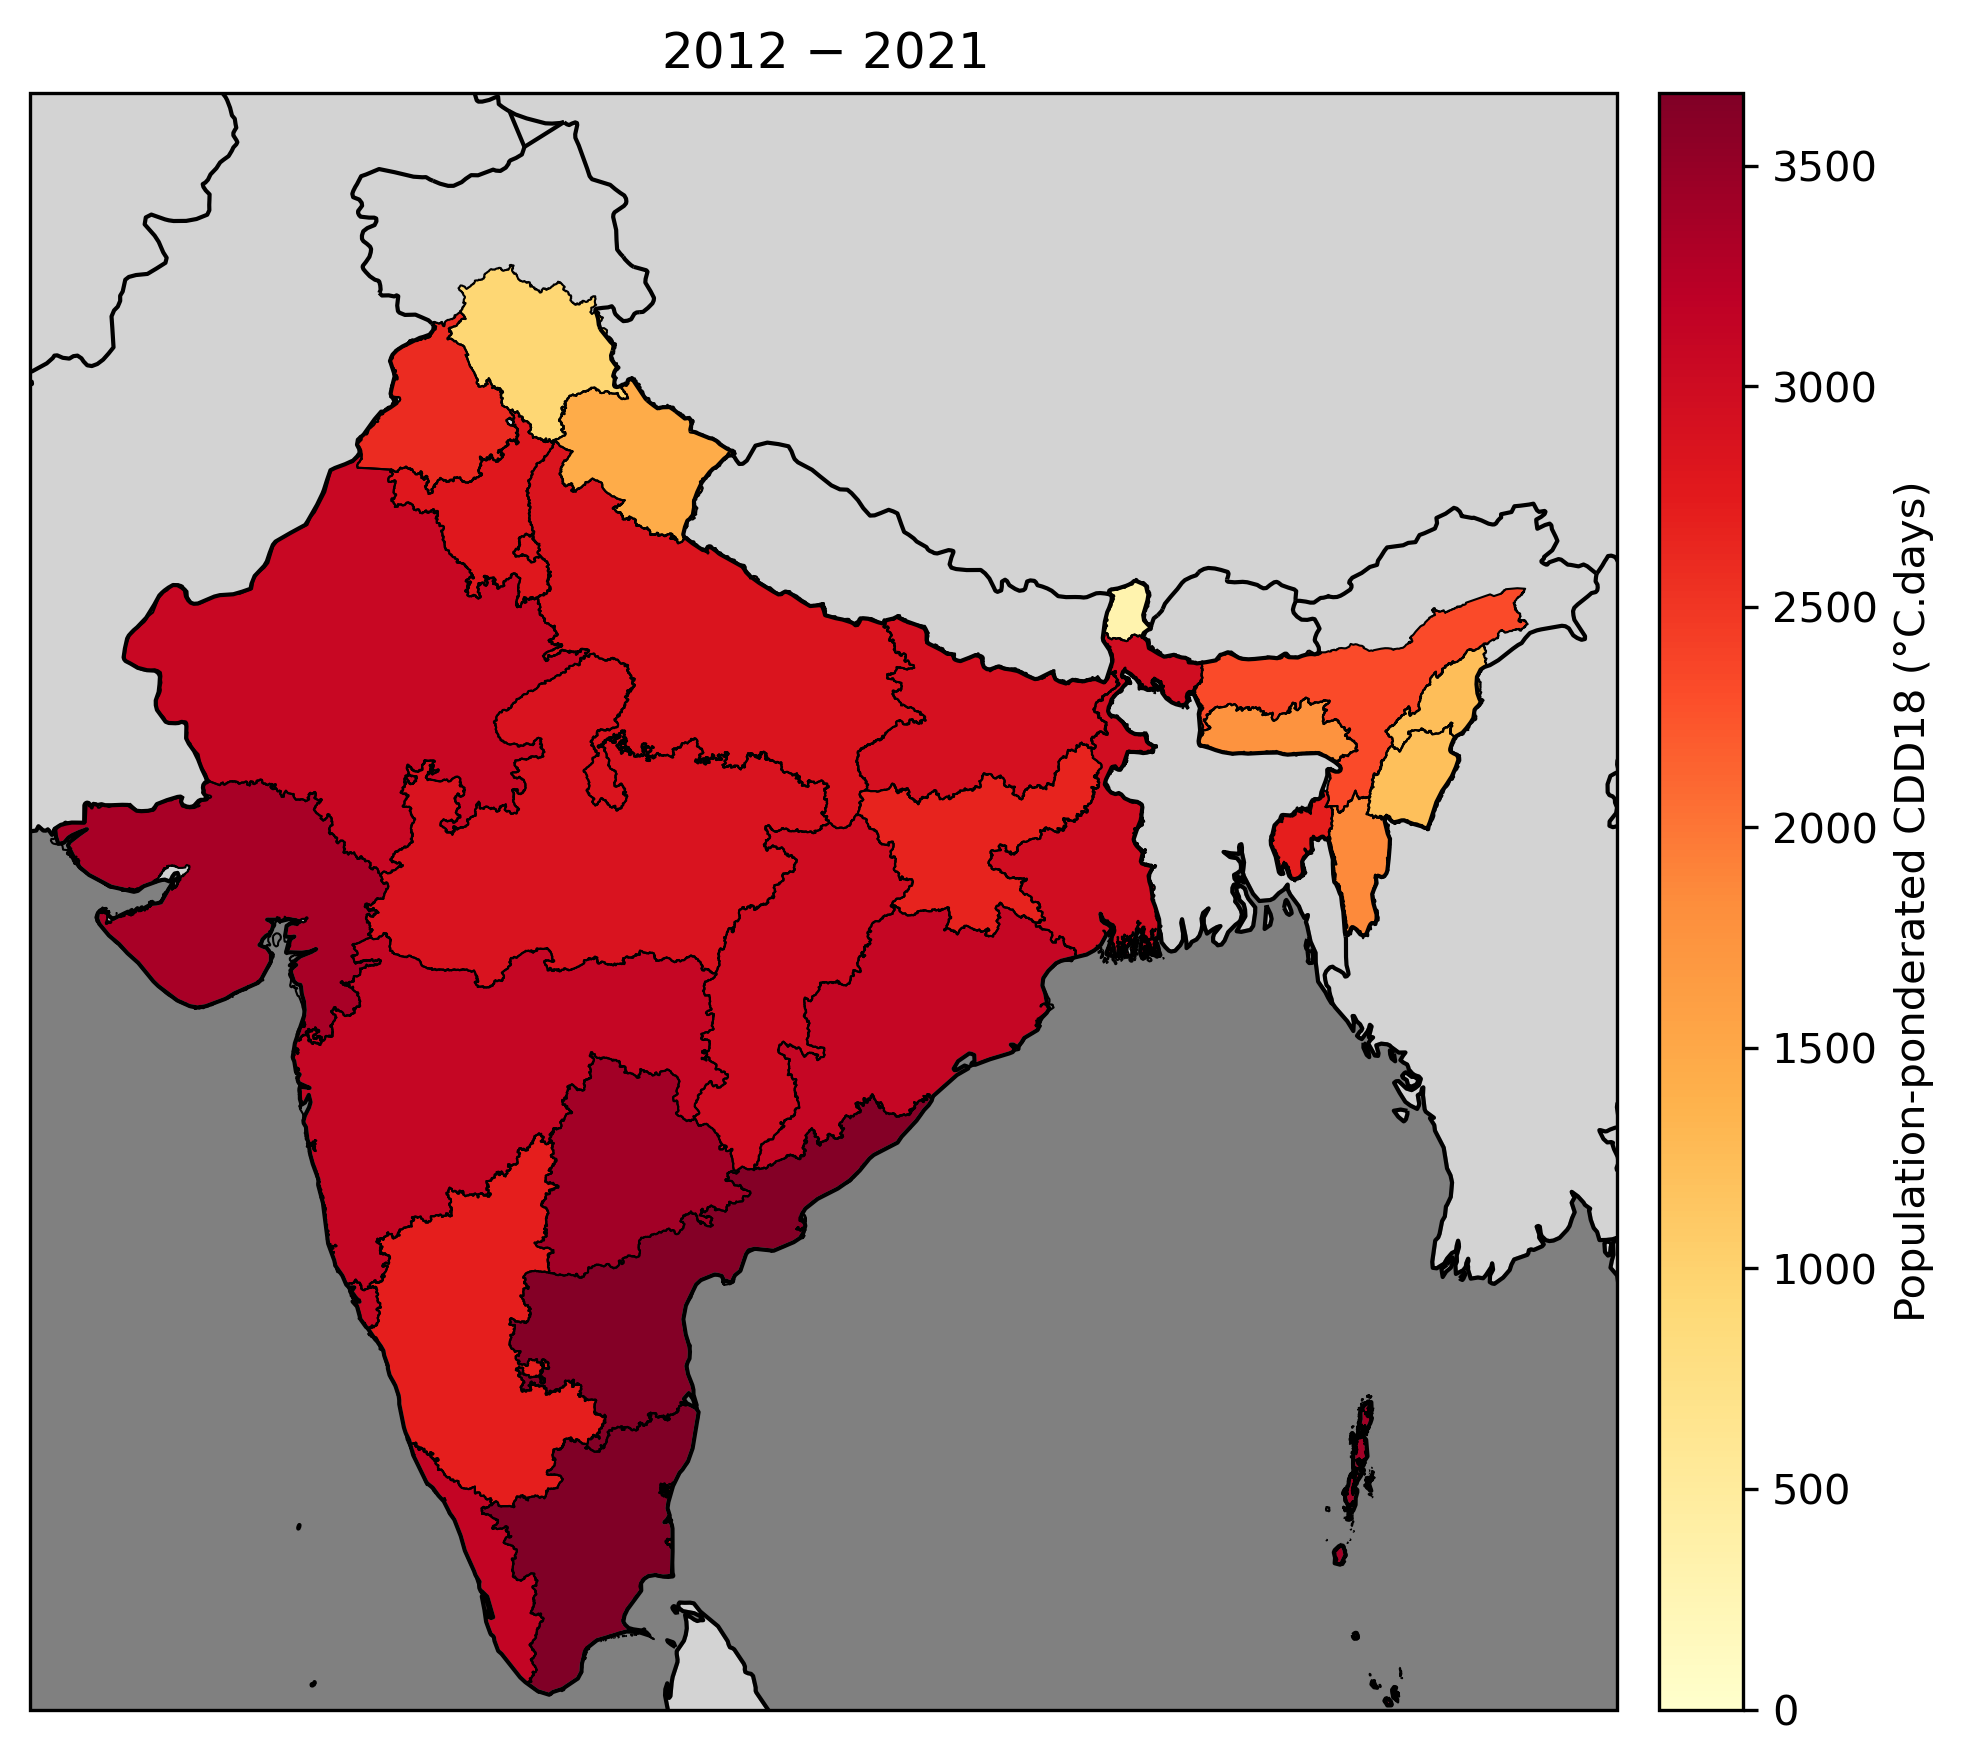
\includegraphics[width=0.49\columnwidth]{figures/20260403_cdd18_2021_period10.png}
   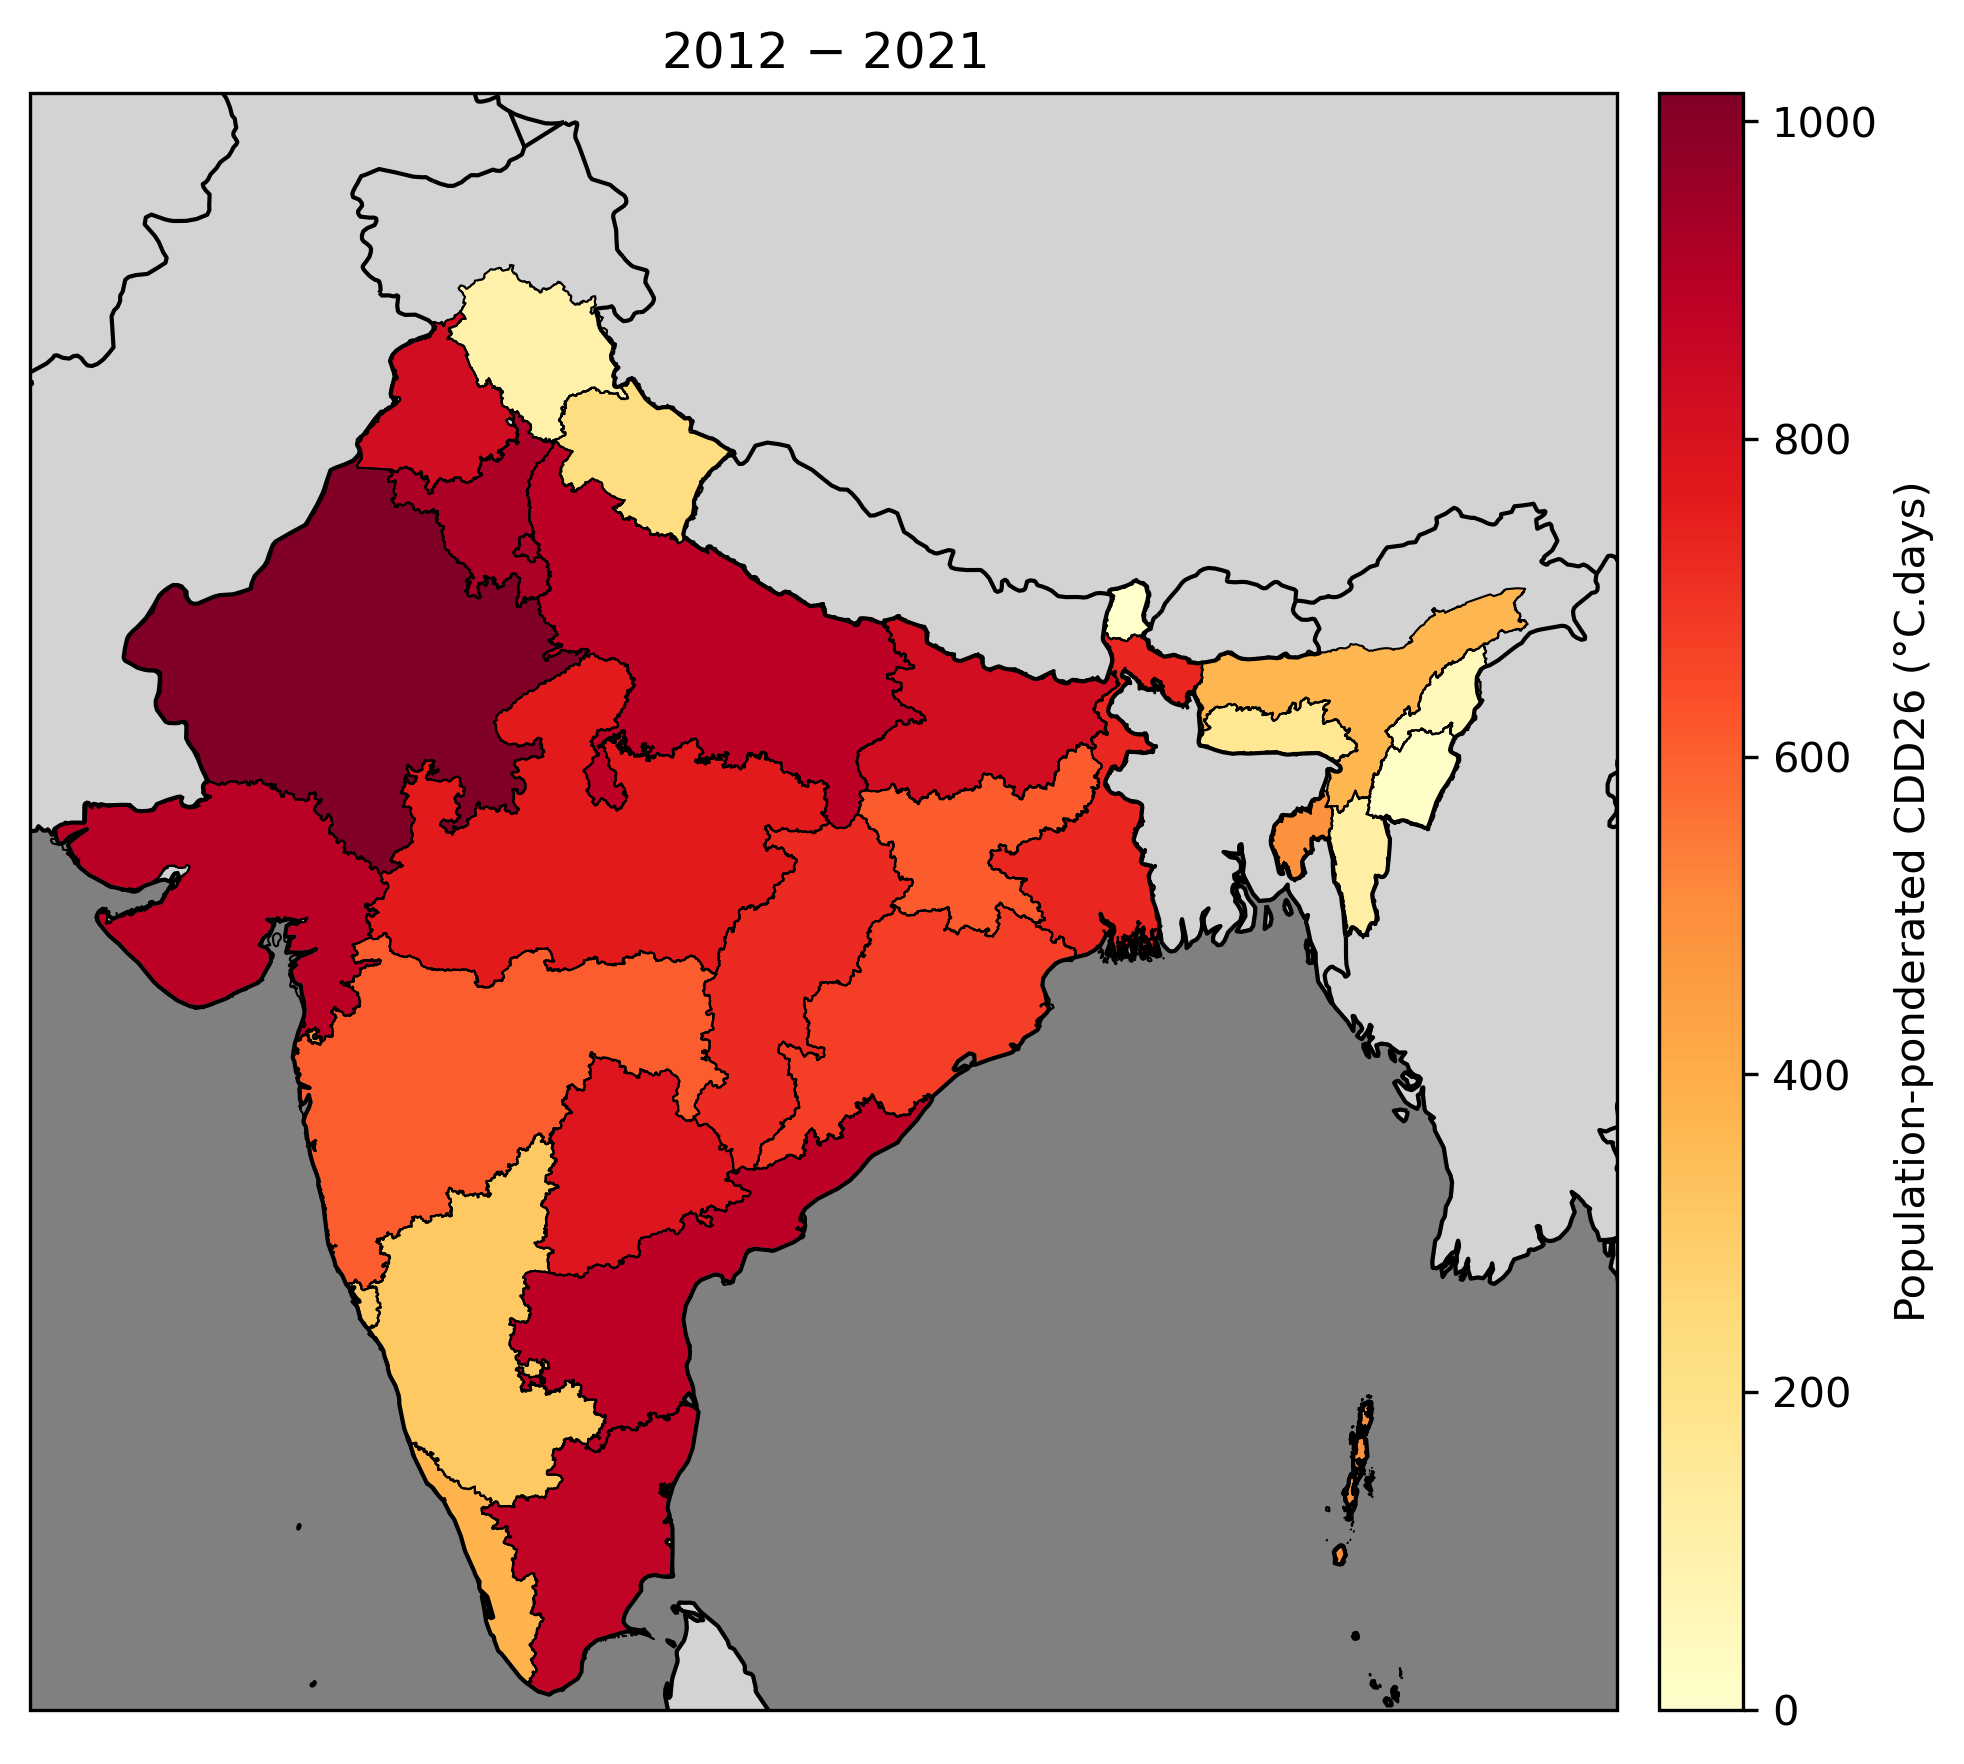
\includegraphics[width=0.49\columnwidth]{figures/20260403_cdd26_2021_period10.png}
   \caption{\label{fig:cdd1826} Carte des CDD18 et CDD26 pondérés par la distribution de population et par état, en moyenne sur la période 2012-2021. Données issues de \textcite{iea_weather_2023}.}
\end{figure}

De plus, la forme fonctionnelle $\mathrm{E-S}$ est relativement arbitraire, se basant principalement sur les premiers travaux de \textcite{sailor_air_2003} et enrichis de ceux de \textcite{mcneil_future_2008}. Nous explorons d'autres formes, combinaisons des formes $\mathrm{E}$ et $\mathrm{S}$ : 
\begin{enumerate}
   % \begin{multicols}{4}
      \item $\mathrm{E-S}$
      \item $\mathrm{S-S}$
      \item $\mathrm{E-E}$
      \item $\mathrm{S-E}$
   % \end{multicols}
\end{enumerate}

\clearpage 
\section{Résultats de modélisation}

Pour l'ensemble des seuils de CDD et les formes fonctionnelles, on résumé les valeurs des paramètres $\alpha$, $\beta$, $\gamma$ et $\delta$ dans la \ref{tab:res}. Ces valeurs sont les résultats de régressions aux moindres carrés réalisés avec la fonction \texttt{curve\_fit} du module Python \texttt{scipy.optimize}. Pour certains modèles, les résultats ne sont pas satisfaisants. Dans ce cas, les modèles sont considérés comme non viables. \\

Les graphes de l'ensemble des modèles et valeurs seuils de CDD sont disponibles dans les sous-sections suivantes. 

\begin{table}[h!]
   \centering
   \caption{\label{tab:res} Résultats des paramètres de modélisation}
   \resizebox{\columnwidth}{!}{
   \begin{tabular}{lclSSSS}
   \toprule
   Modèle & Paramètres & Unités & \multicolumn{1}{r}{CDD18} & \multicolumn{1}{r}{CDD21} & \multicolumn{1}{r}{CDD23}& \multicolumn{1}{r}{CDD26}\\
   \midrule
   $\mathrm{E-S}$ & $\alpha$ & \SI{}{\per\degreeday} & 1.22e-04 & 1.76e-04 & 2.70e-04 & 1.45e-03 \\
    & $\beta$ & \SI{}{\degreeday}& 2.86e+02 & 7.04e+01 & 2.15e+01 & -2.40e+01 \\
   & $\gamma$ & \SI{}{\per\indianrupee} & 1.86e-05 & 1.81e-05 & 1.72e-05 & 1.34e-05 \\
   & $\delta$ & \SI{}{\indianrupee}& 2.08e+05 & 2.12e+05 & 2.22e+05 & 3.10e+05 \\
   \cline{2-7}\\[-3mm]
   & $R^2$ & -- & 0.567 & 0.590 & 0.607 & 0.578 \\
   \ref{fig:es}& Modèle viable & -- & \checkmark & \checkmark & \checkmark & \checkmark \\
   \midrule

   $\mathrm{S-S}$ & $\alpha$ & \SI{}{\per\degreeday} & 1.10e-01 & 4.41e-02 & 3.43e-03 & 6.11e-03 \\
   & $\beta$ & \SI{}{\degreeday}& 2.35e+03 & 1.67e+03 & 1.05e+03 & 3.40e+02 \\
   & $\gamma$ & \SI{}{\per\indianrupee} & 8.01e-06 & 7.81e-06 & 9.82e-06 & 1.29e-05 \\
   & $\delta$ & \SI{}{\indianrupee}& 4.56e+05 & 4.55e+05 & 3.79e+05 & 3.42e+05 \\
   \cline{2-7}\\[-3mm]
   & $R^2$ & -- & 0.574 & 0.614 & 0.584 & 0.560 \\
   \ref{fig:ss}& Modèle viable & -- &  &  & \checkmark & \checkmark \\
   \midrule 

   $\mathrm{E-E}$ & $\alpha$ & \SI{}{\per\degreeday} & 7.02e-04 & 7.46e-04 & 1.04e-03 & 4.97e-03 \\
   & $\beta$ & \SI{}{\degreeday}& 3.83e+02 & 1.18e+02 & 5.43e+01 & -6.08e+00 \\
   & $\gamma$ & \SI{}{\per\indianrupee} & 1.15e-06 & 1.30e-06 & 1.33e-06 & 1.08e-06 \\
   & $\delta$ & \SI{}{\indianrupee}& 5.62e+04 & 5.56e+04 & 5.57e+04 & 5.92e+04 \\
   \cline{2-7}\\[-3mm]
   & $R^2$ & -- & 0.554 & 0.569 & 0.582 & 0.527 \\
   \ref{fig:ee}& Modèle viable & -- & \checkmark & \checkmark & \checkmark & \checkmark \\

   \midrule
   $\mathrm{S-E}$ & $\alpha$ & \SI{}{\per\degreeday} & 6.67e-02 & 5.58e-02 & 2.21e-01 & 4.07e-01 \\
   & $\beta$ & \SI{}{\degreeday}& 2.34e+03 & 1.66e+03 & 9.65e+02 & 1.27e+02 \\
   & $\gamma$ & \SI{}{\per\indianrupee} & 9.69e-07 & 1.03e-06 & 1.03e-06 & 9.69e-07 \\
   & $\delta$ & \SI{}{\indianrupee}& 5.05e+04 & 5.01e+04 & 5.02e+04 & 5.63e+04 \\
   \cline{2-7}\\[-3mm]
   & $R^2$ & -- & 0.611 & 0.672 & 0.672 & 0.572 \\
   \ref{fig:se}& Modèle viable & -- &  &  &  &  \\
   \bottomrule

   \end{tabular}
   }
\end{table}

Par cohérence avec la littérature, il pourrait être préférable d'utiliser les modèles $\mathrm{E-S}$. Les valeurs de coefficients des différents seuils de CDD peuvent être utilisés comme des alternatives pour prendre en compte la sensibilité des projections. 

\clearpage 
\subsection{Modèle $\mathrm{E-S}$}
\begin{figure}[ht]
   \centering
   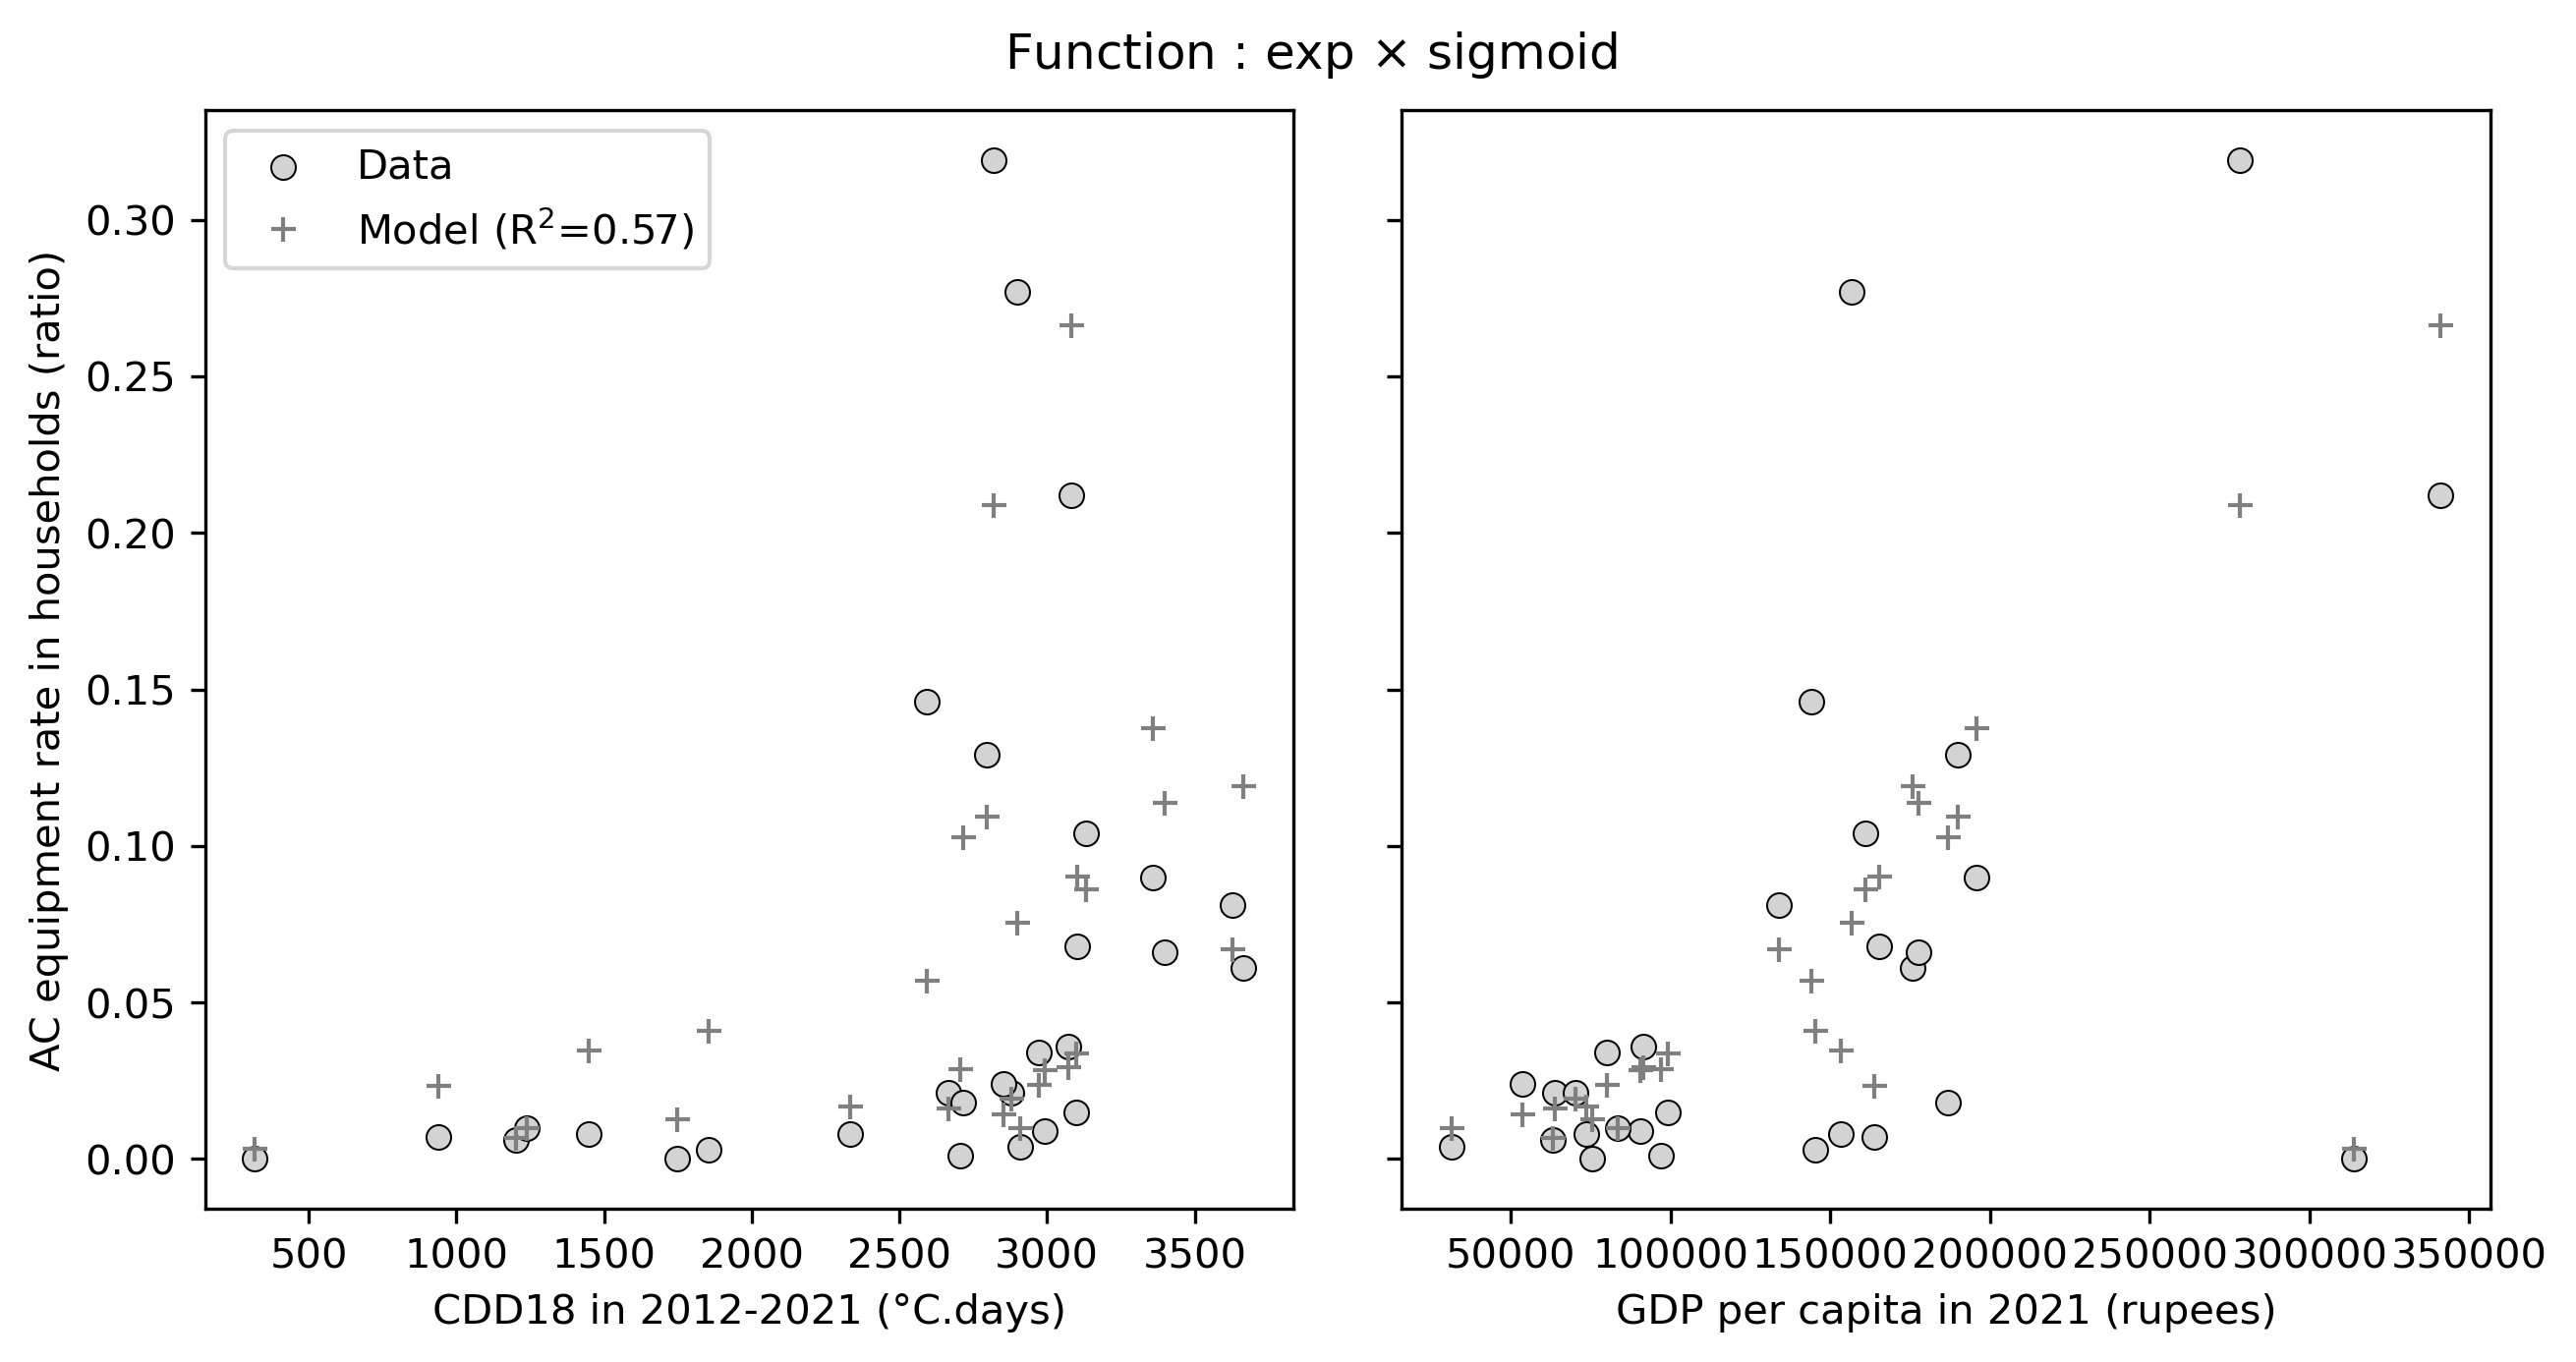
\includegraphics[width=0.6\columnwidth]{figures/cdd18_exp_sigmoid_scatter.png}
   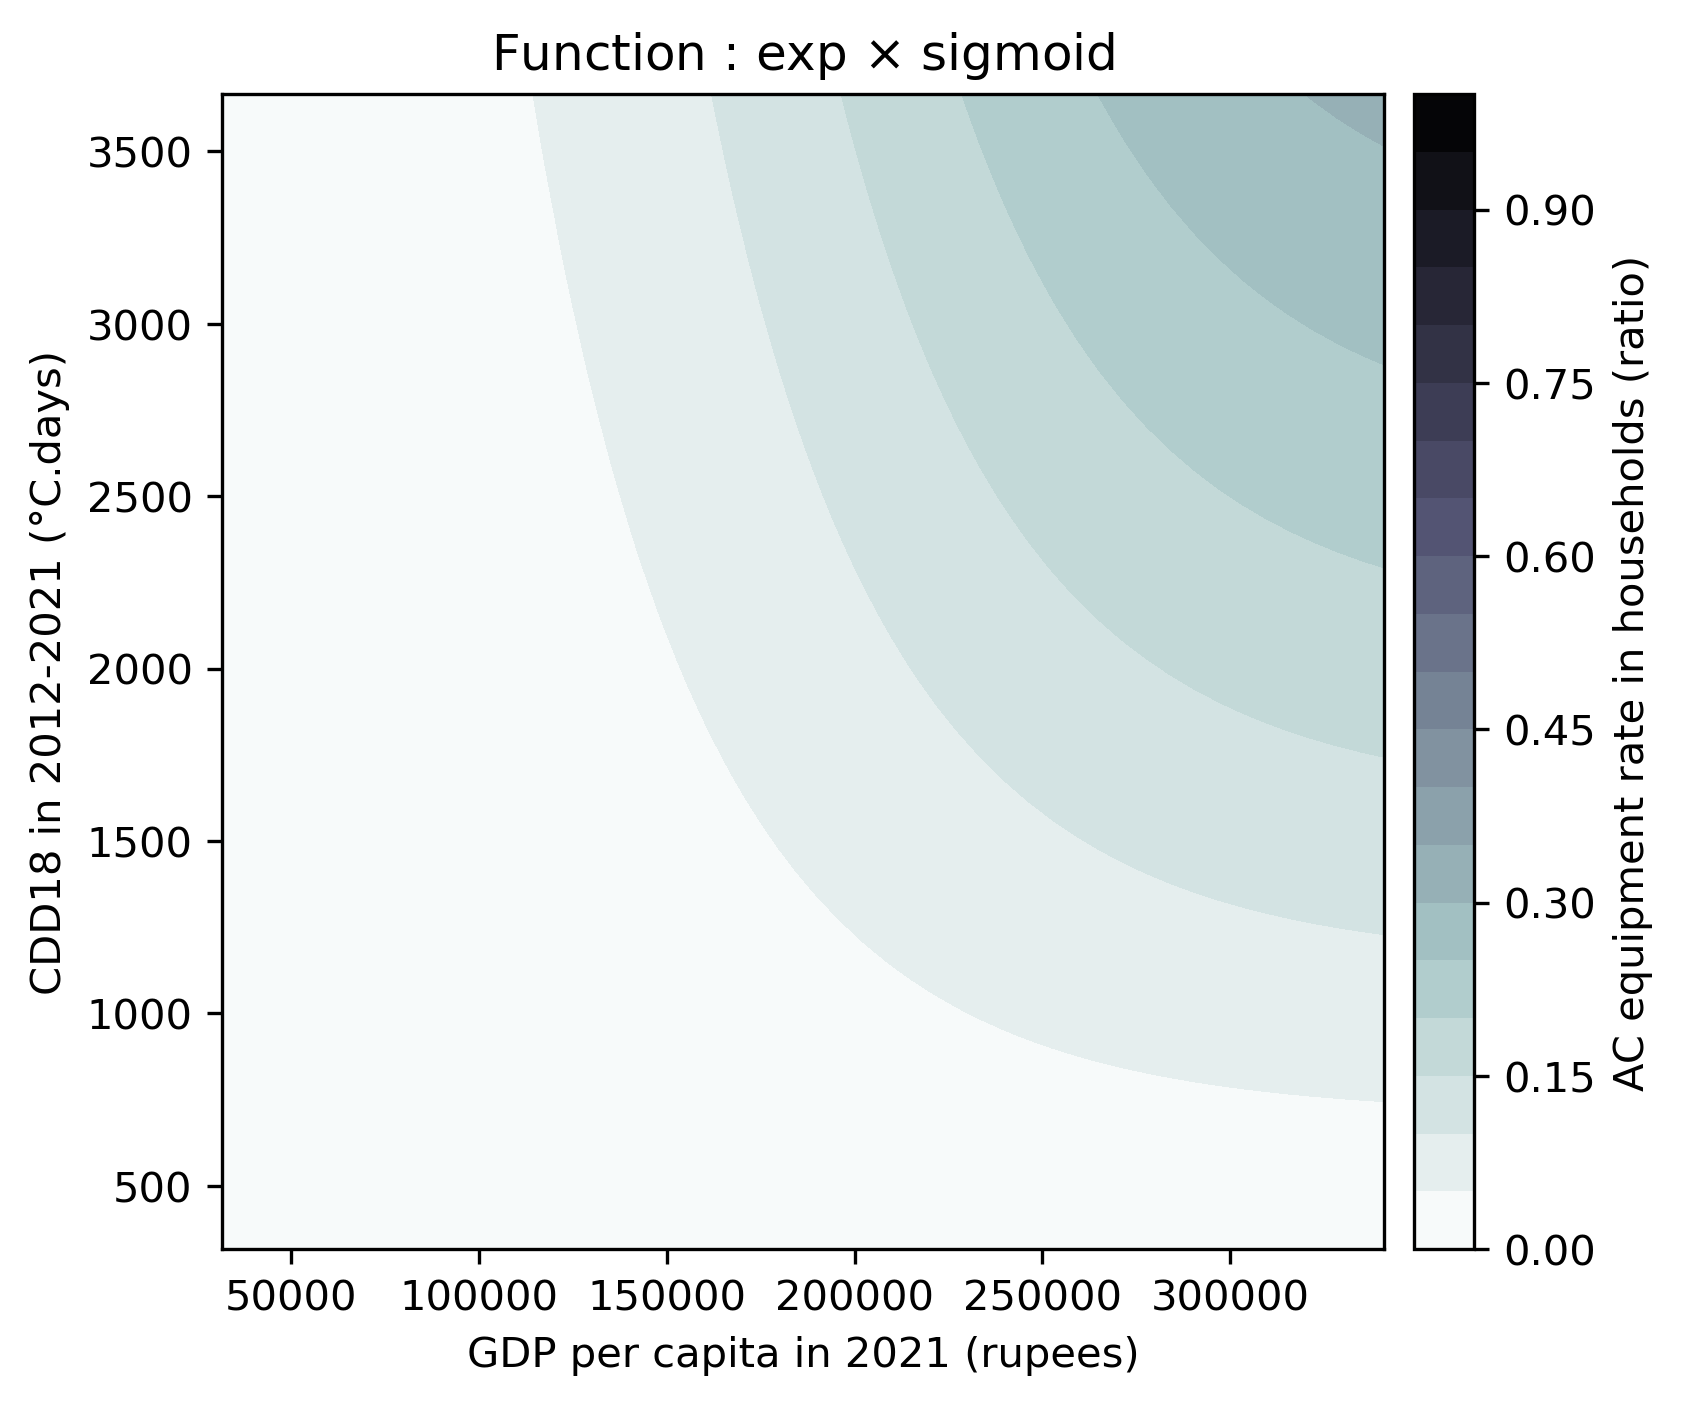
\includegraphics[width=0.38\columnwidth]{figures/cdd18_exp_sigmoid_2dplot.png}

   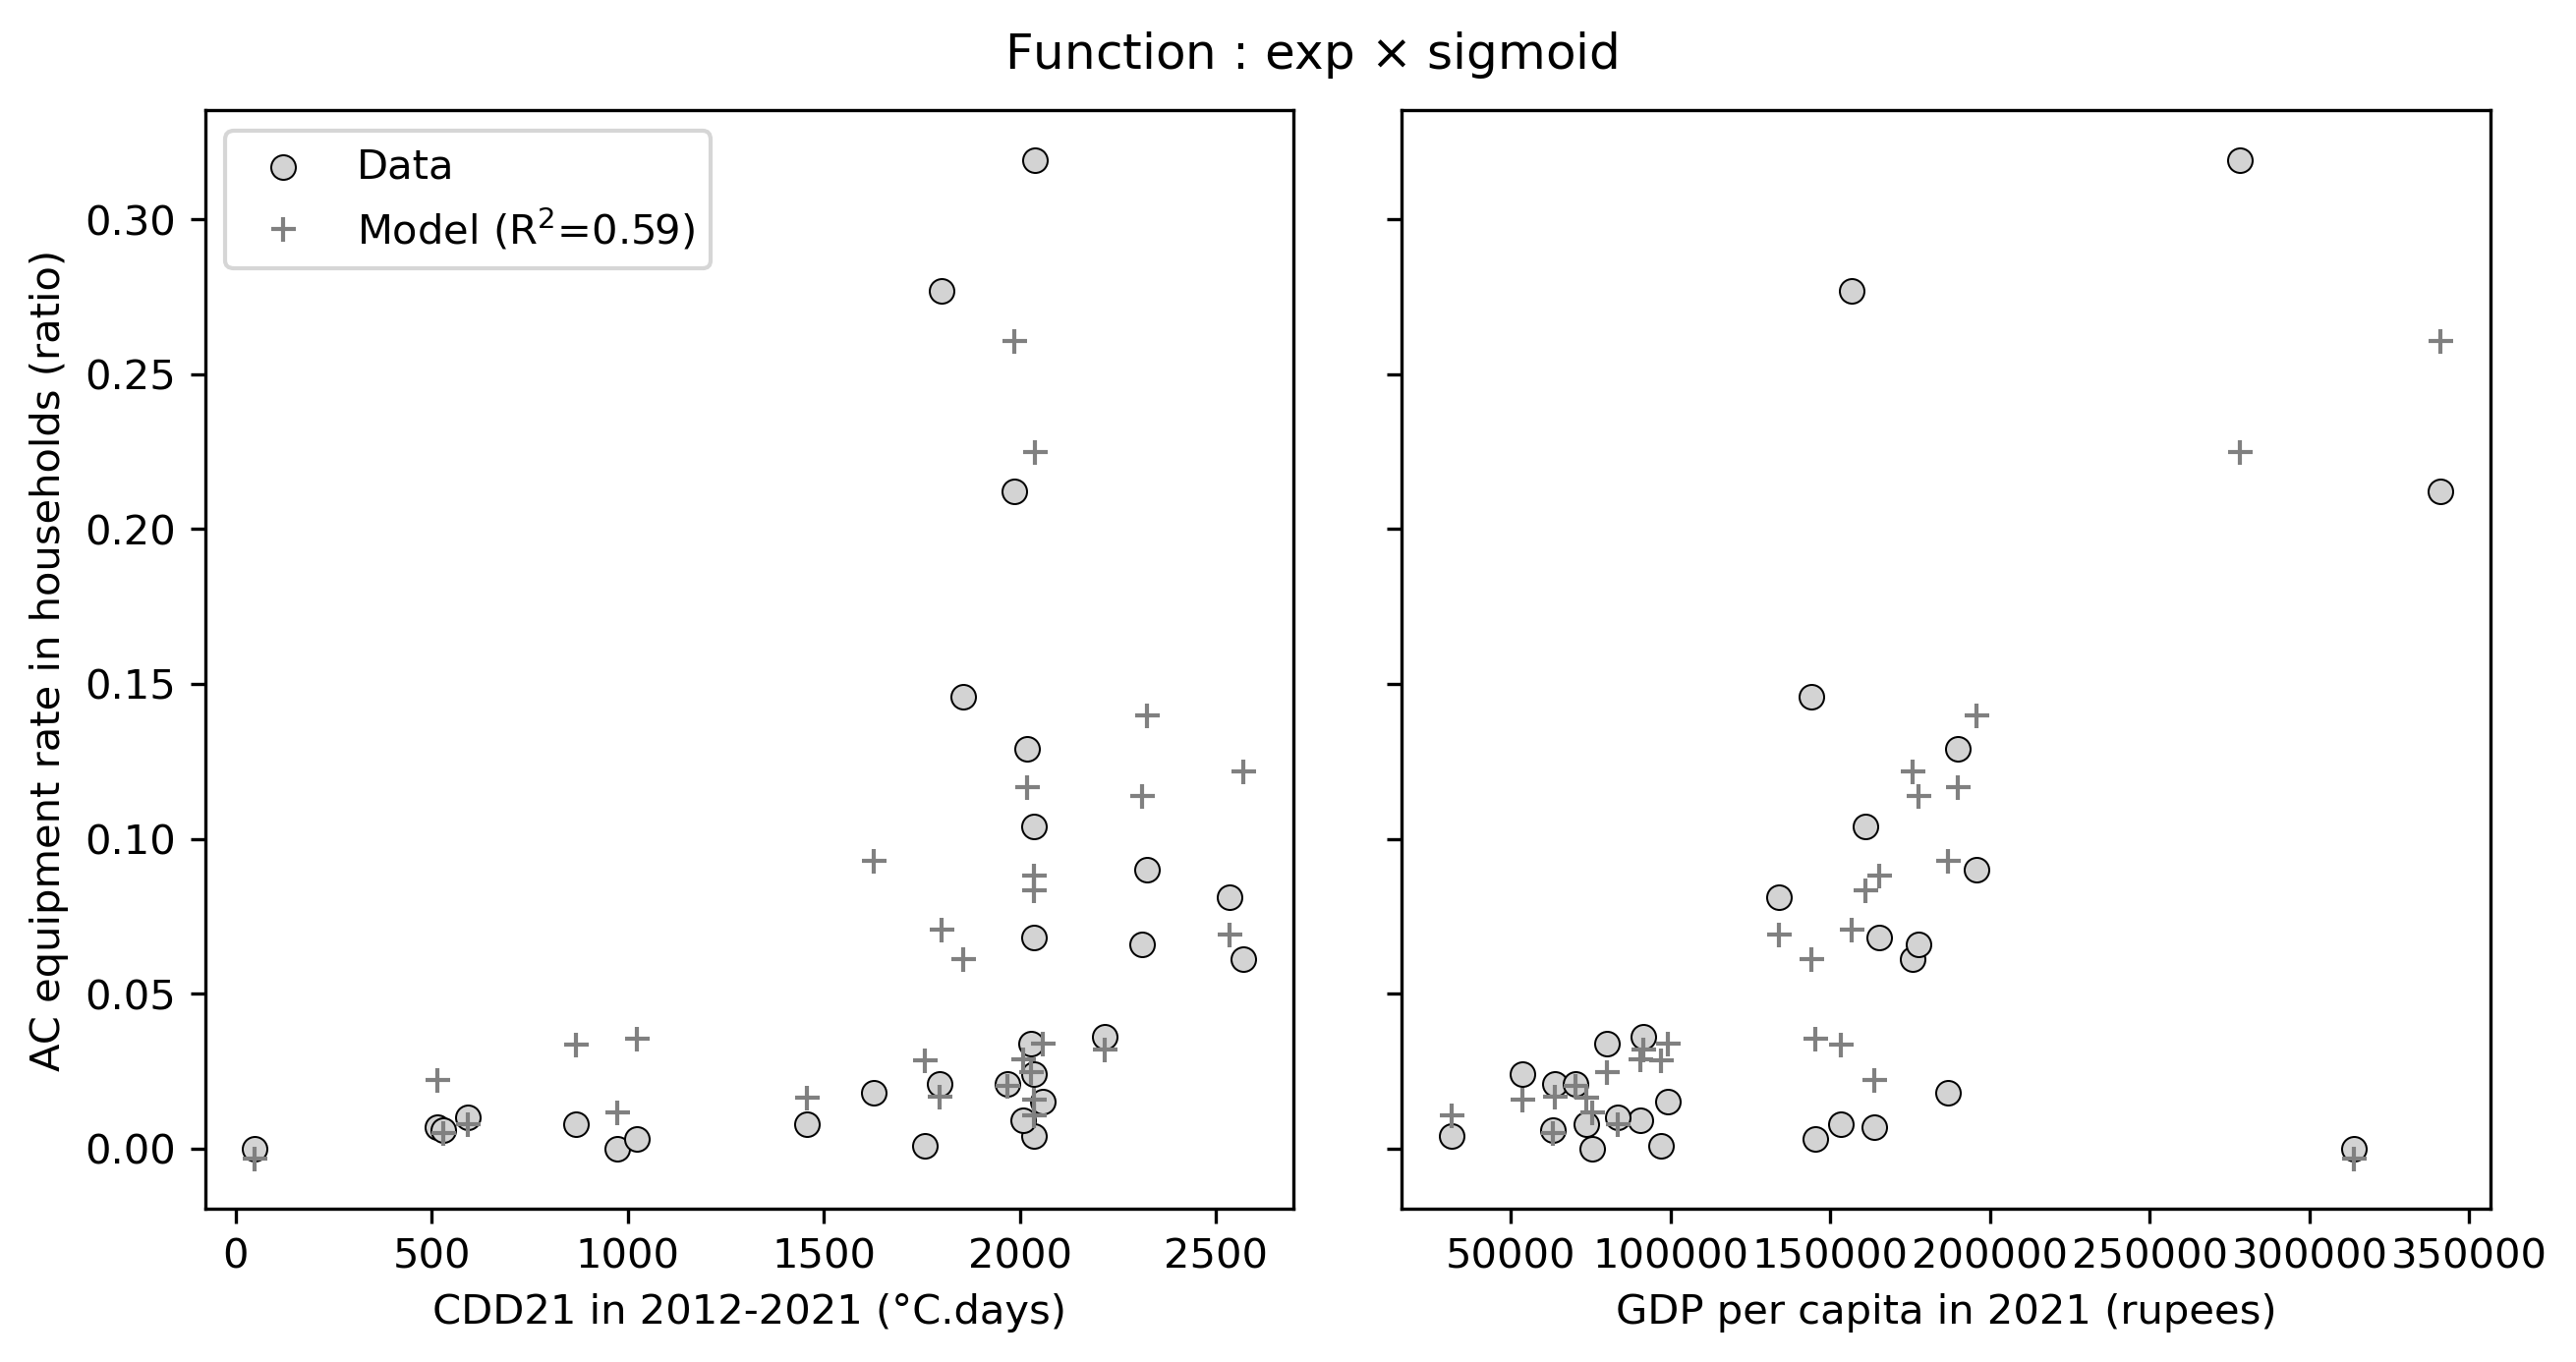
\includegraphics[width=0.6\columnwidth]{figures/cdd21_exp_sigmoid_scatter.png}
   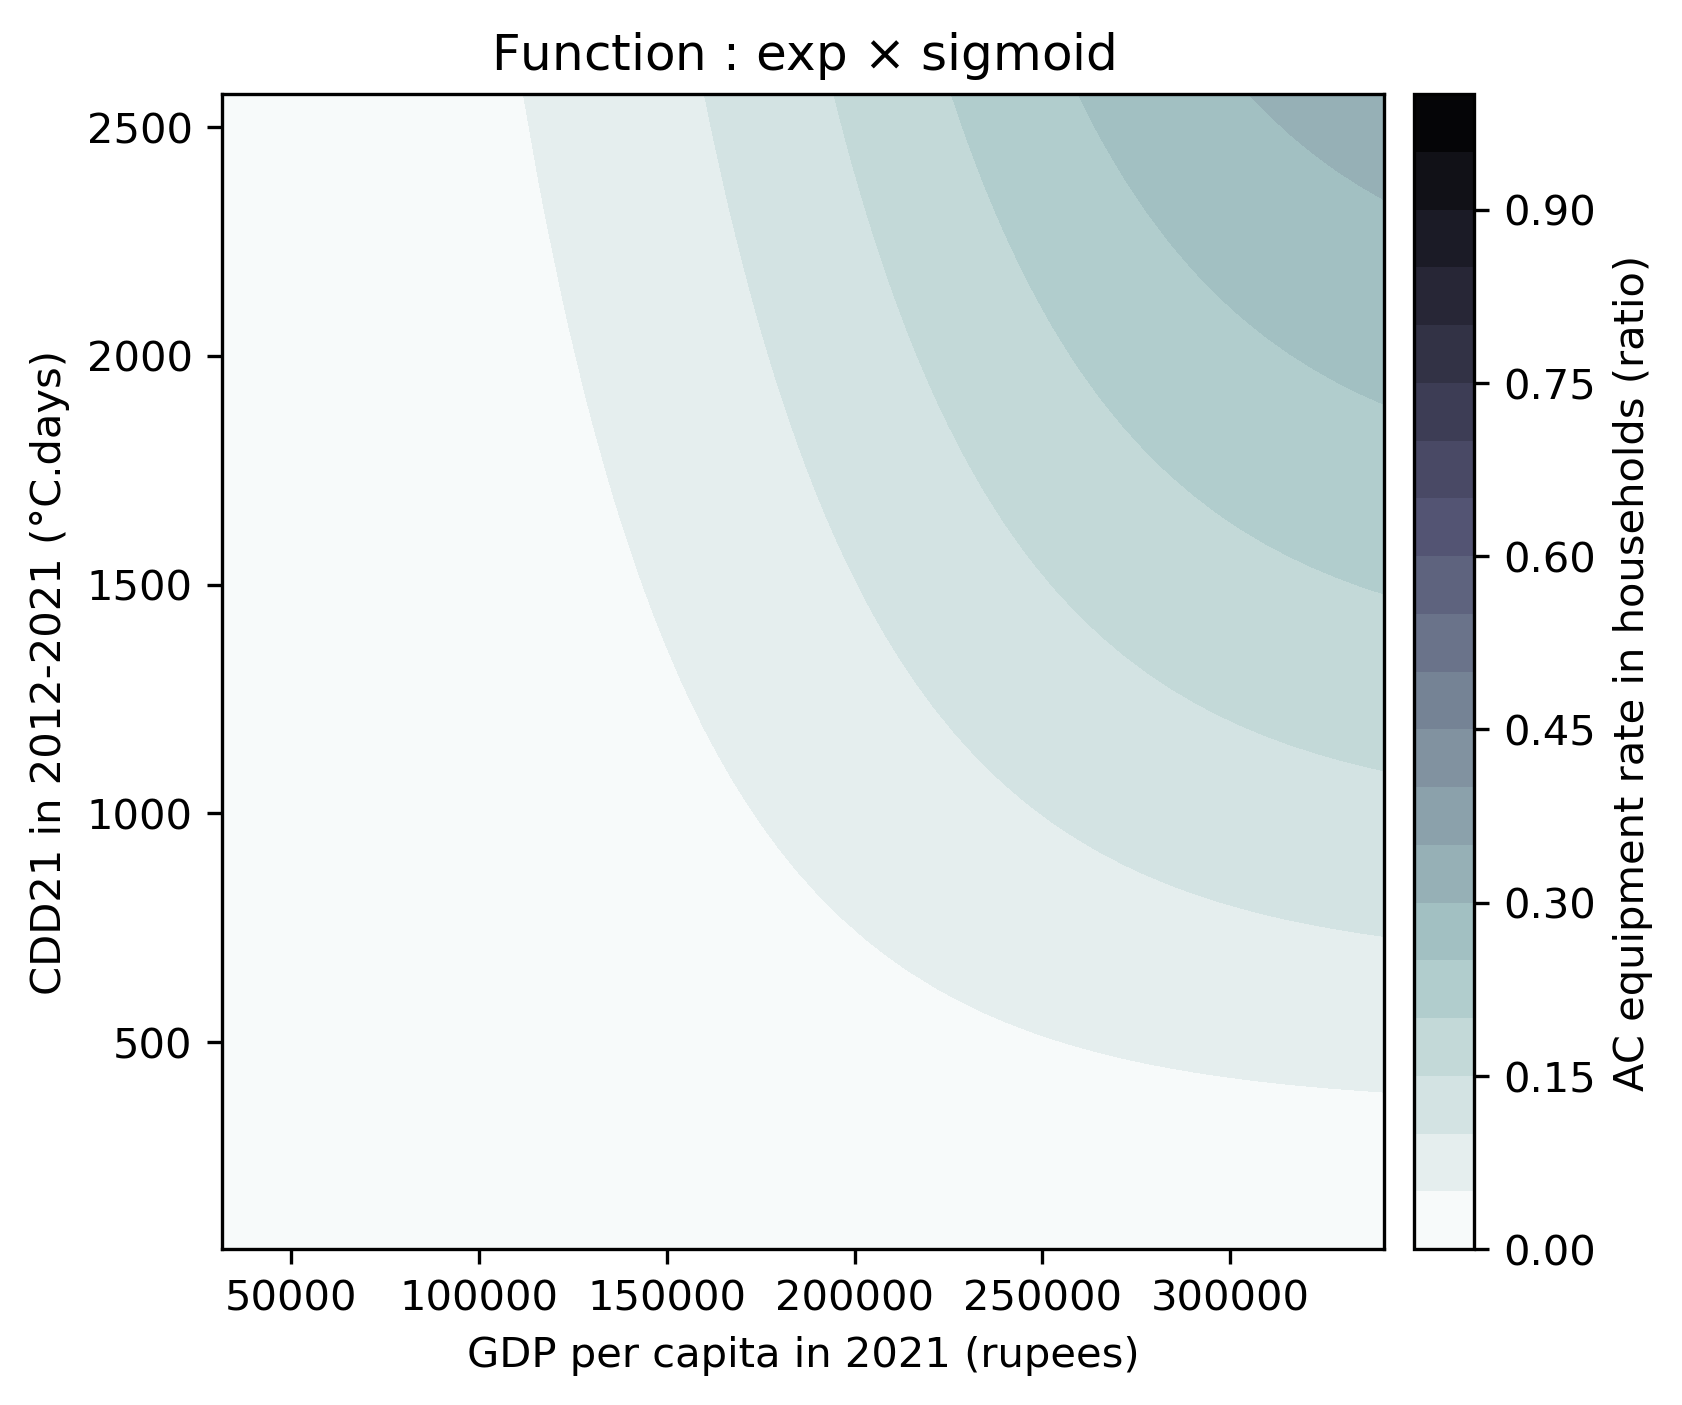
\includegraphics[width=0.38\columnwidth]{figures/cdd21_exp_sigmoid_2dplot.png}

   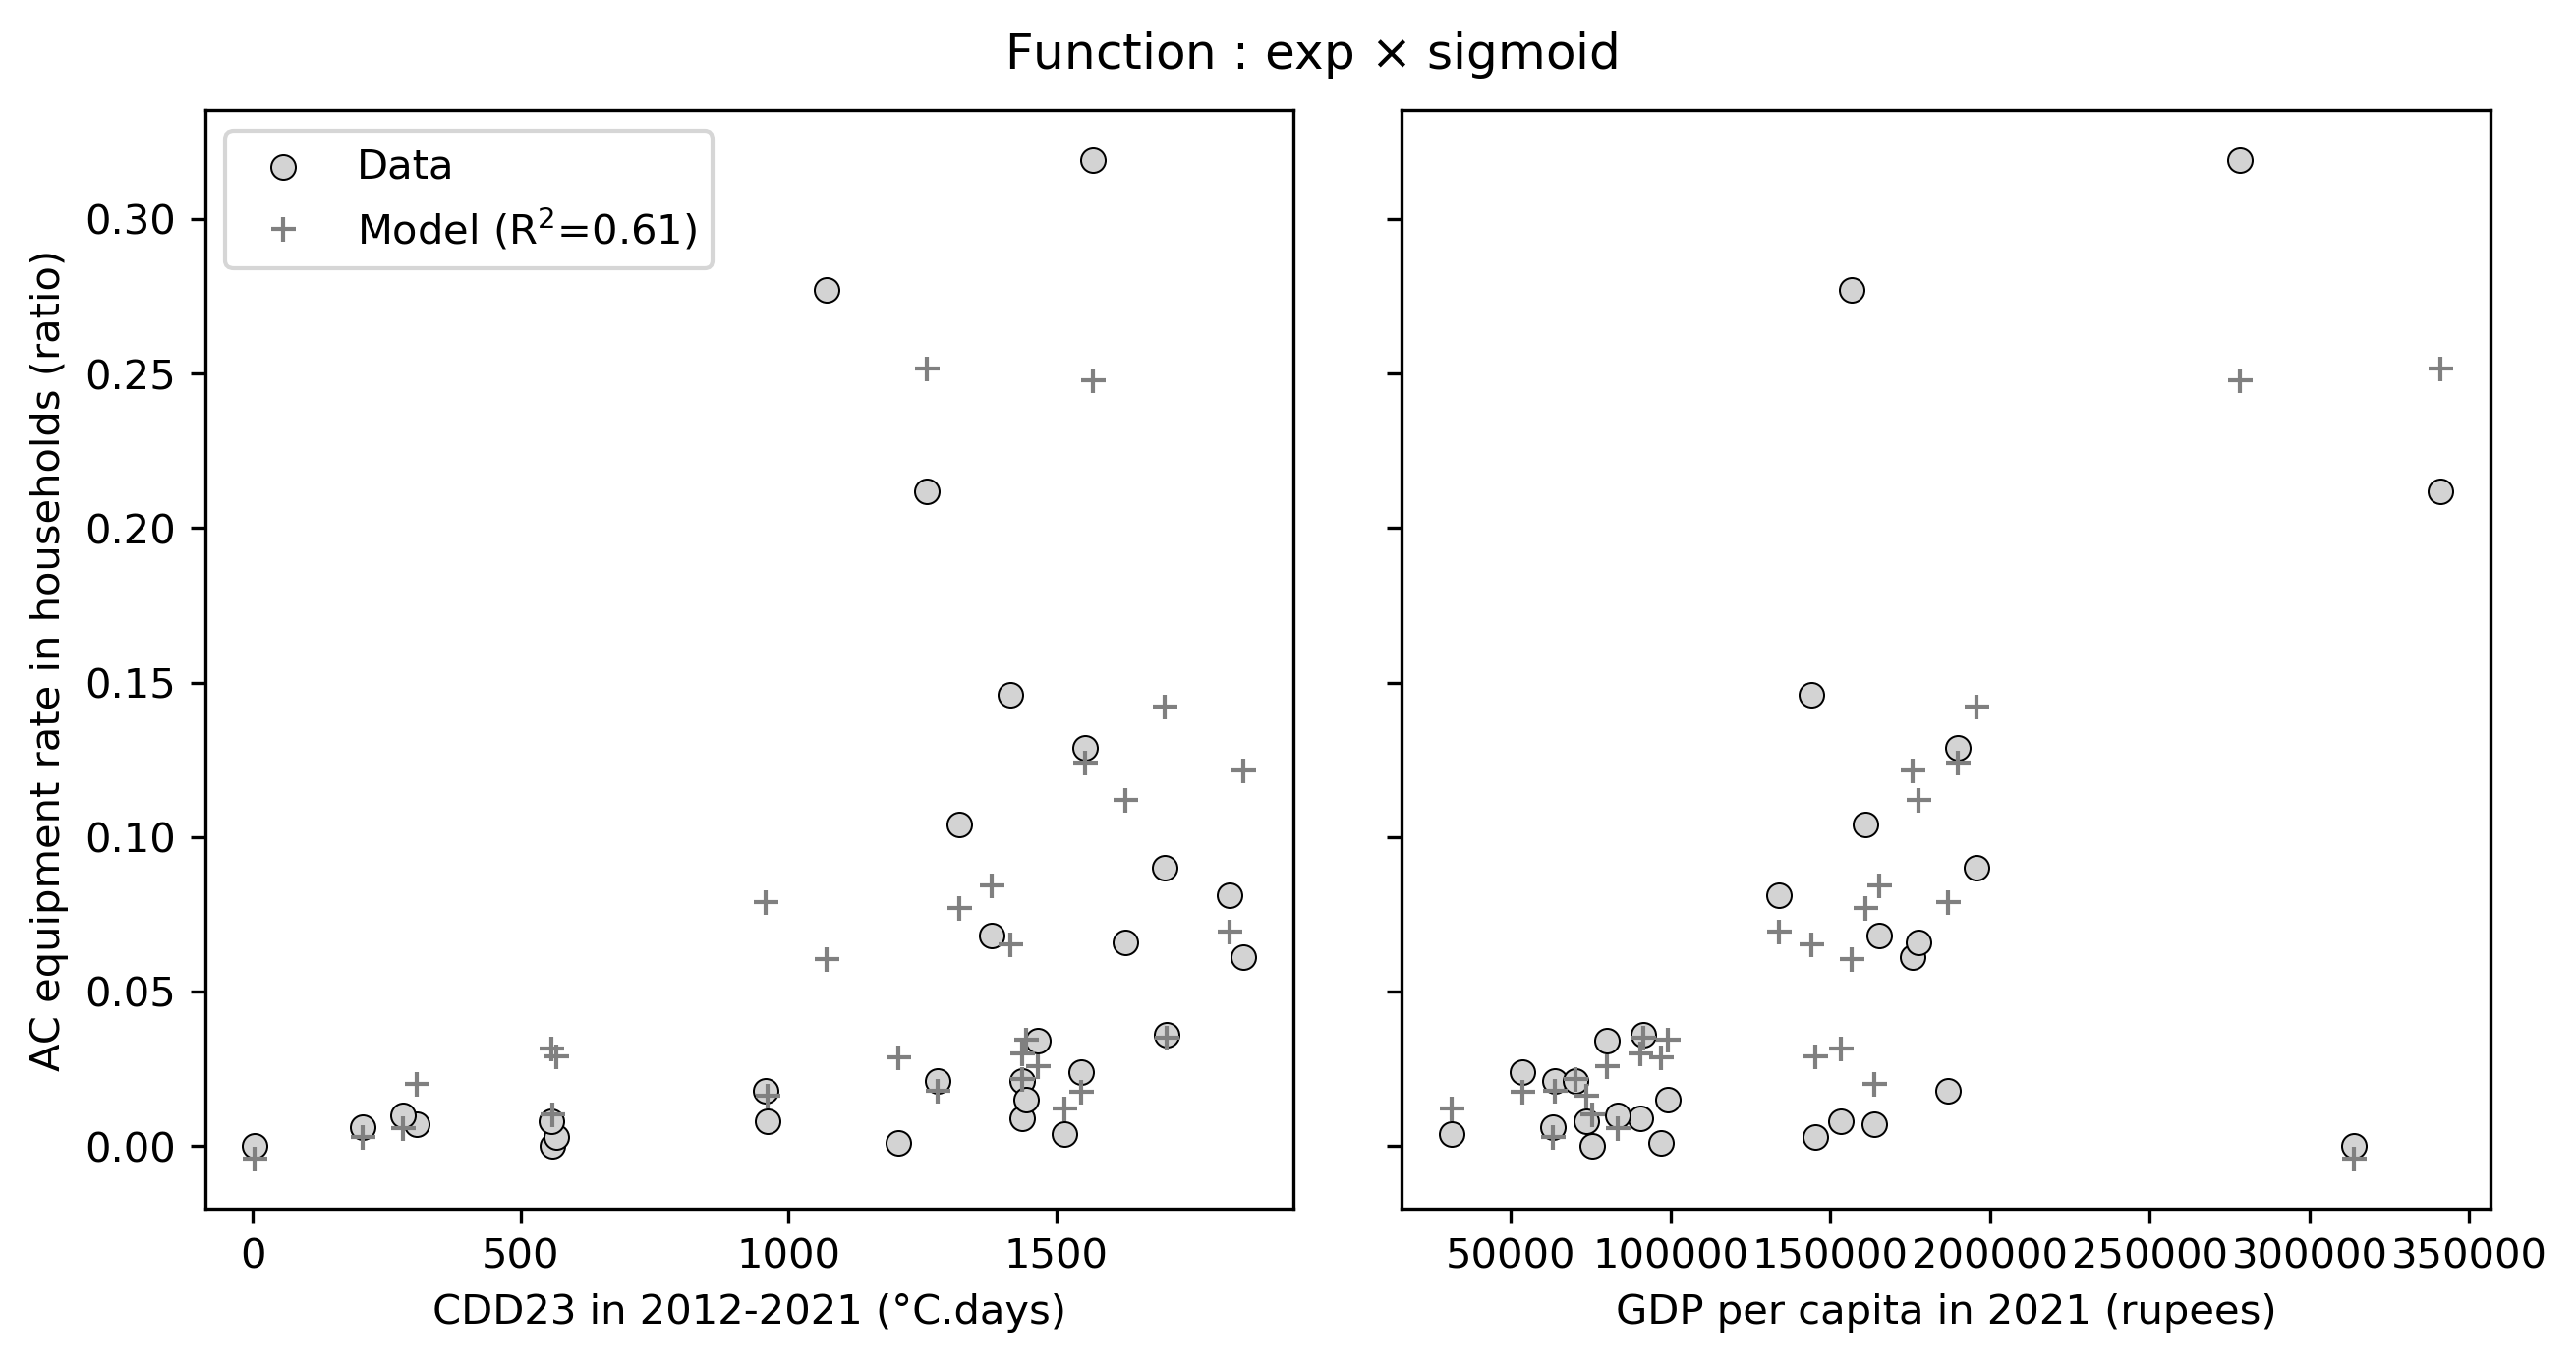
\includegraphics[width=0.6\columnwidth]{figures/cdd23_exp_sigmoid_scatter.png}
   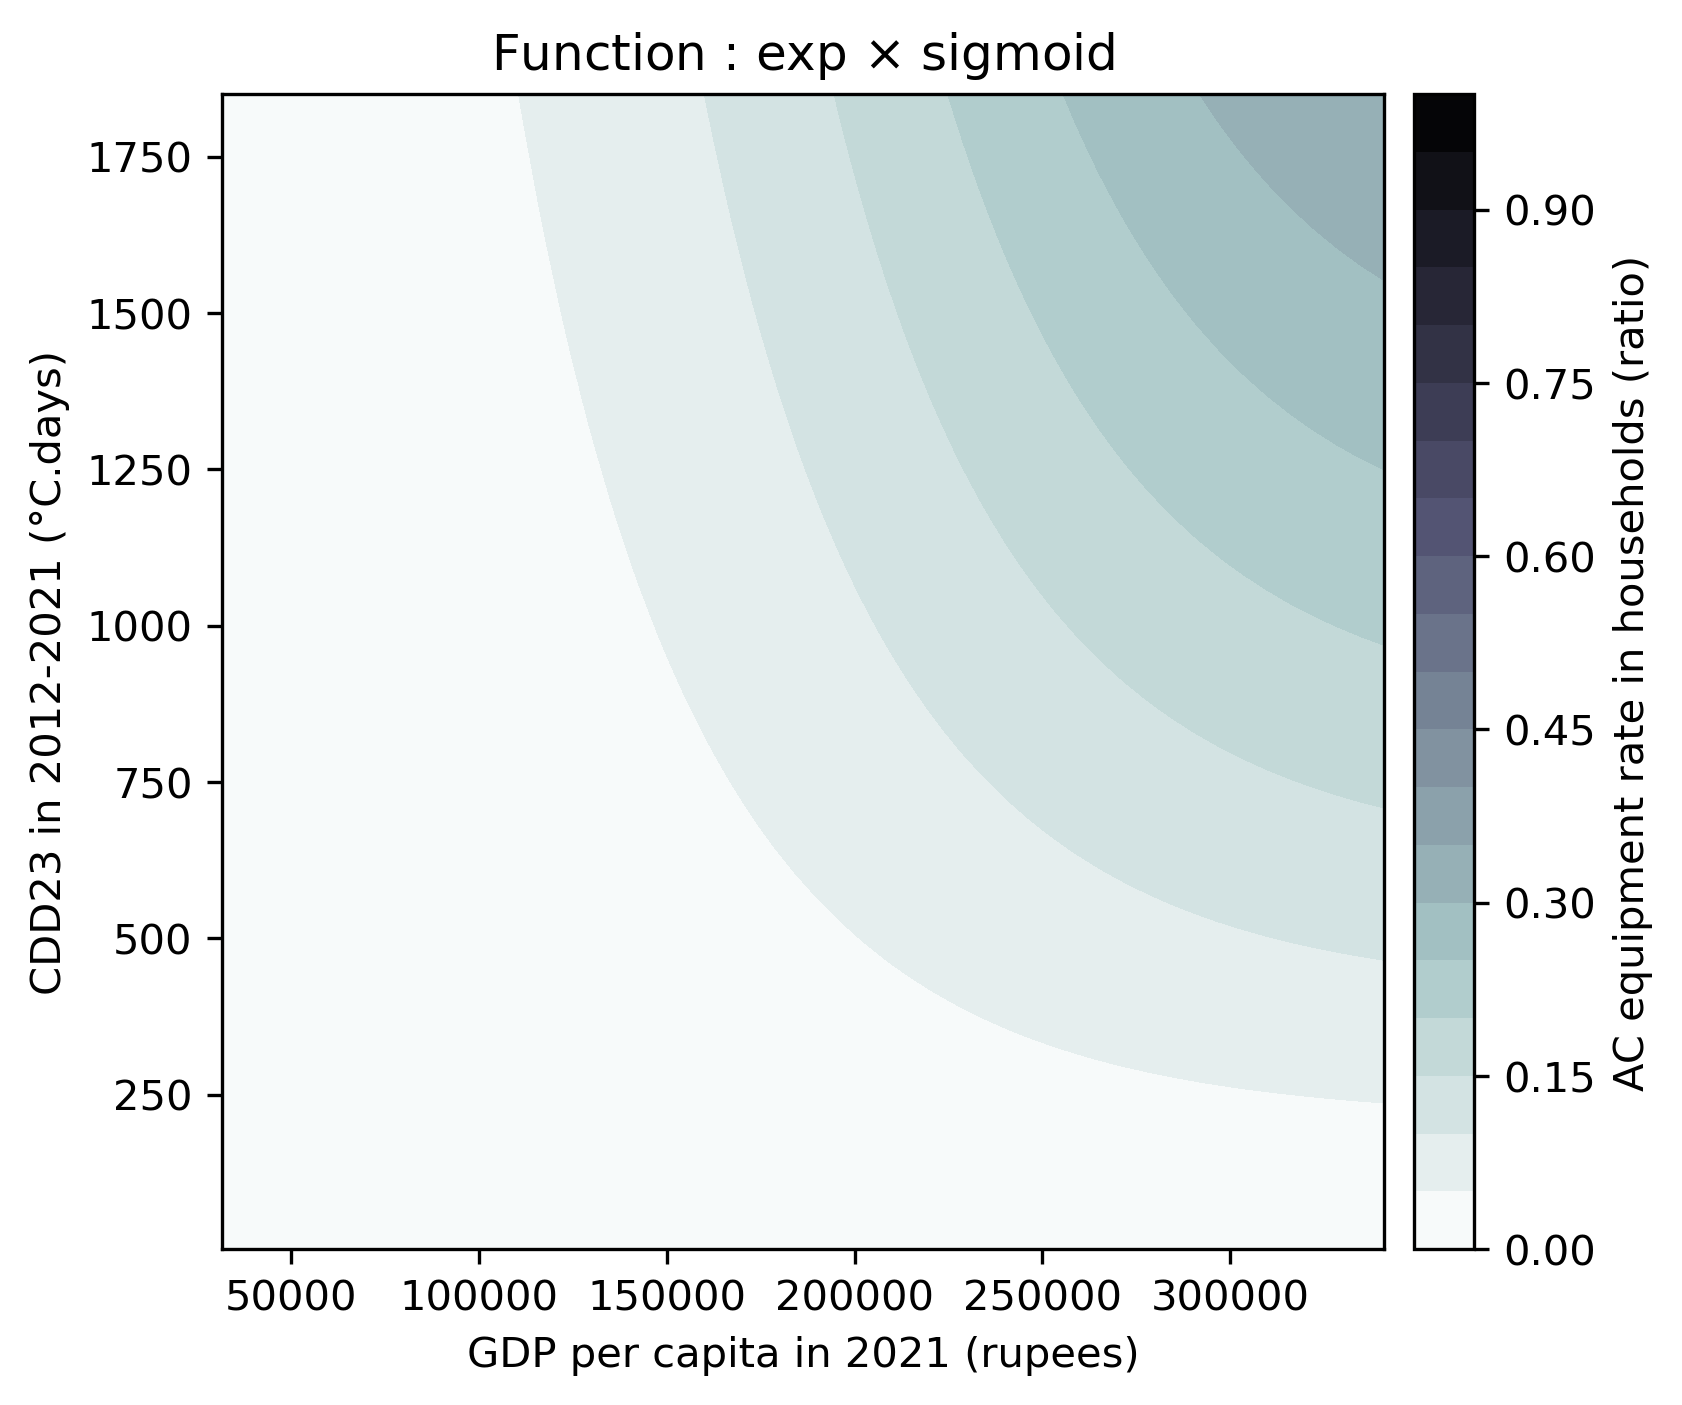
\includegraphics[width=0.38\columnwidth]{figures/cdd23_exp_sigmoid_2dplot.png}

   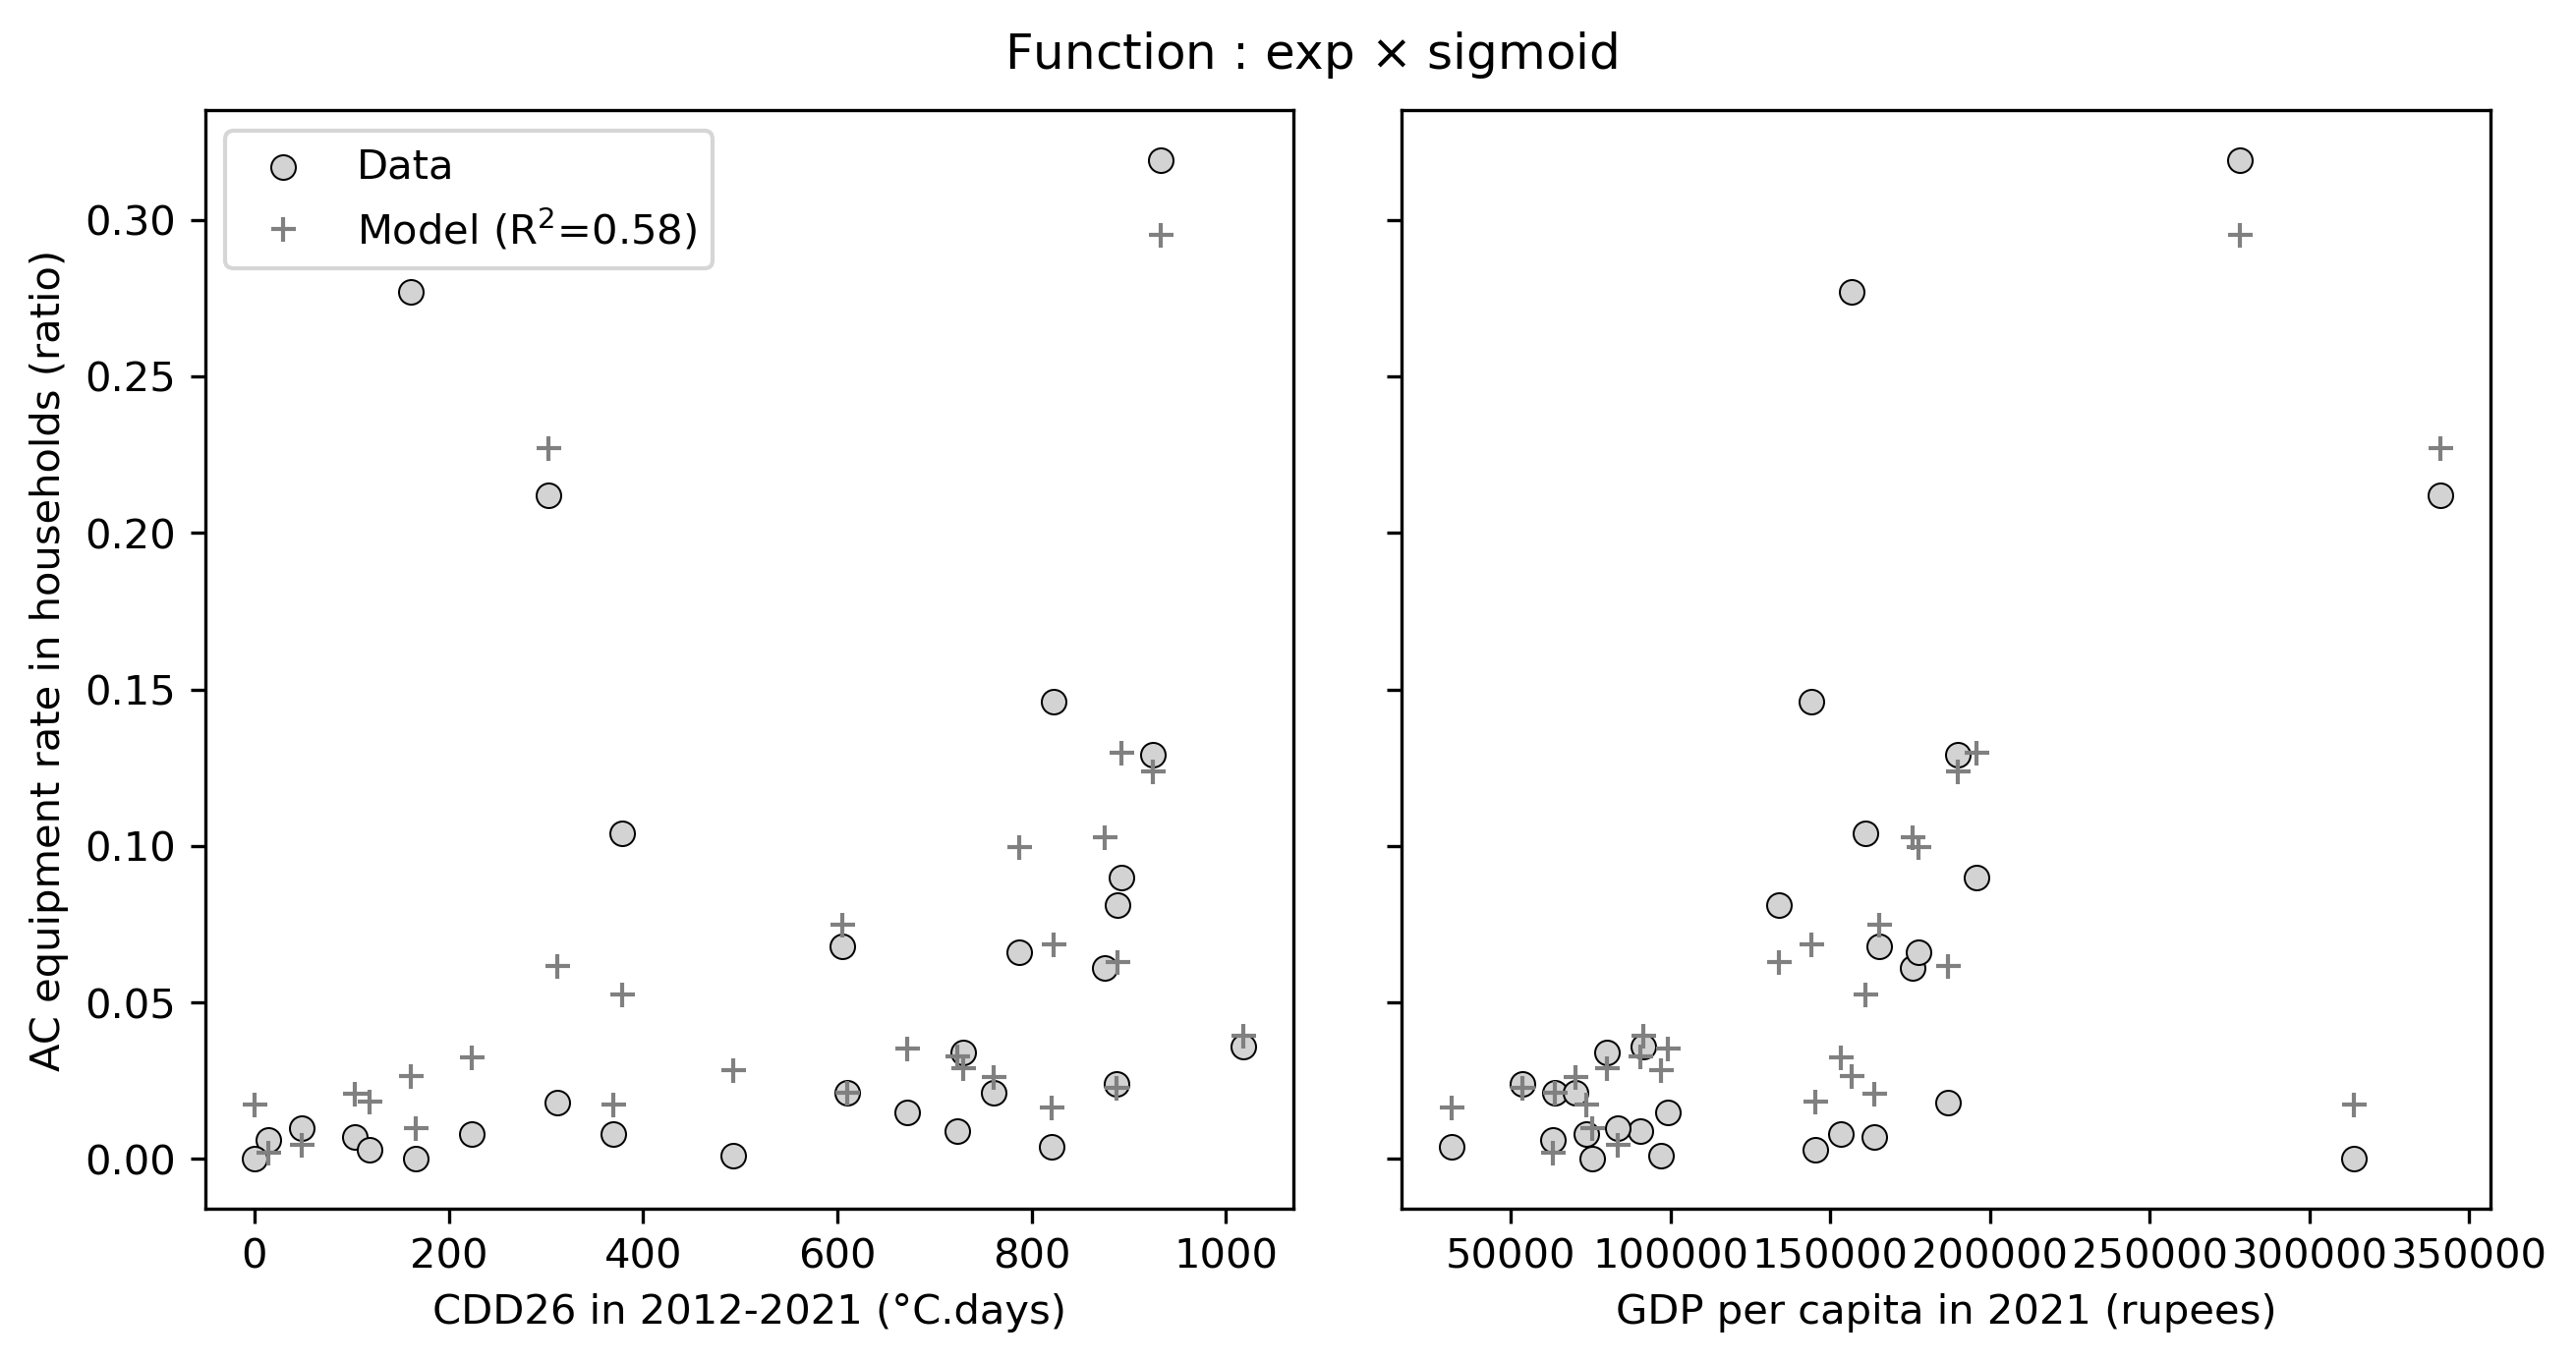
\includegraphics[width=0.6\columnwidth]{figures/cdd26_exp_sigmoid_scatter.png}
   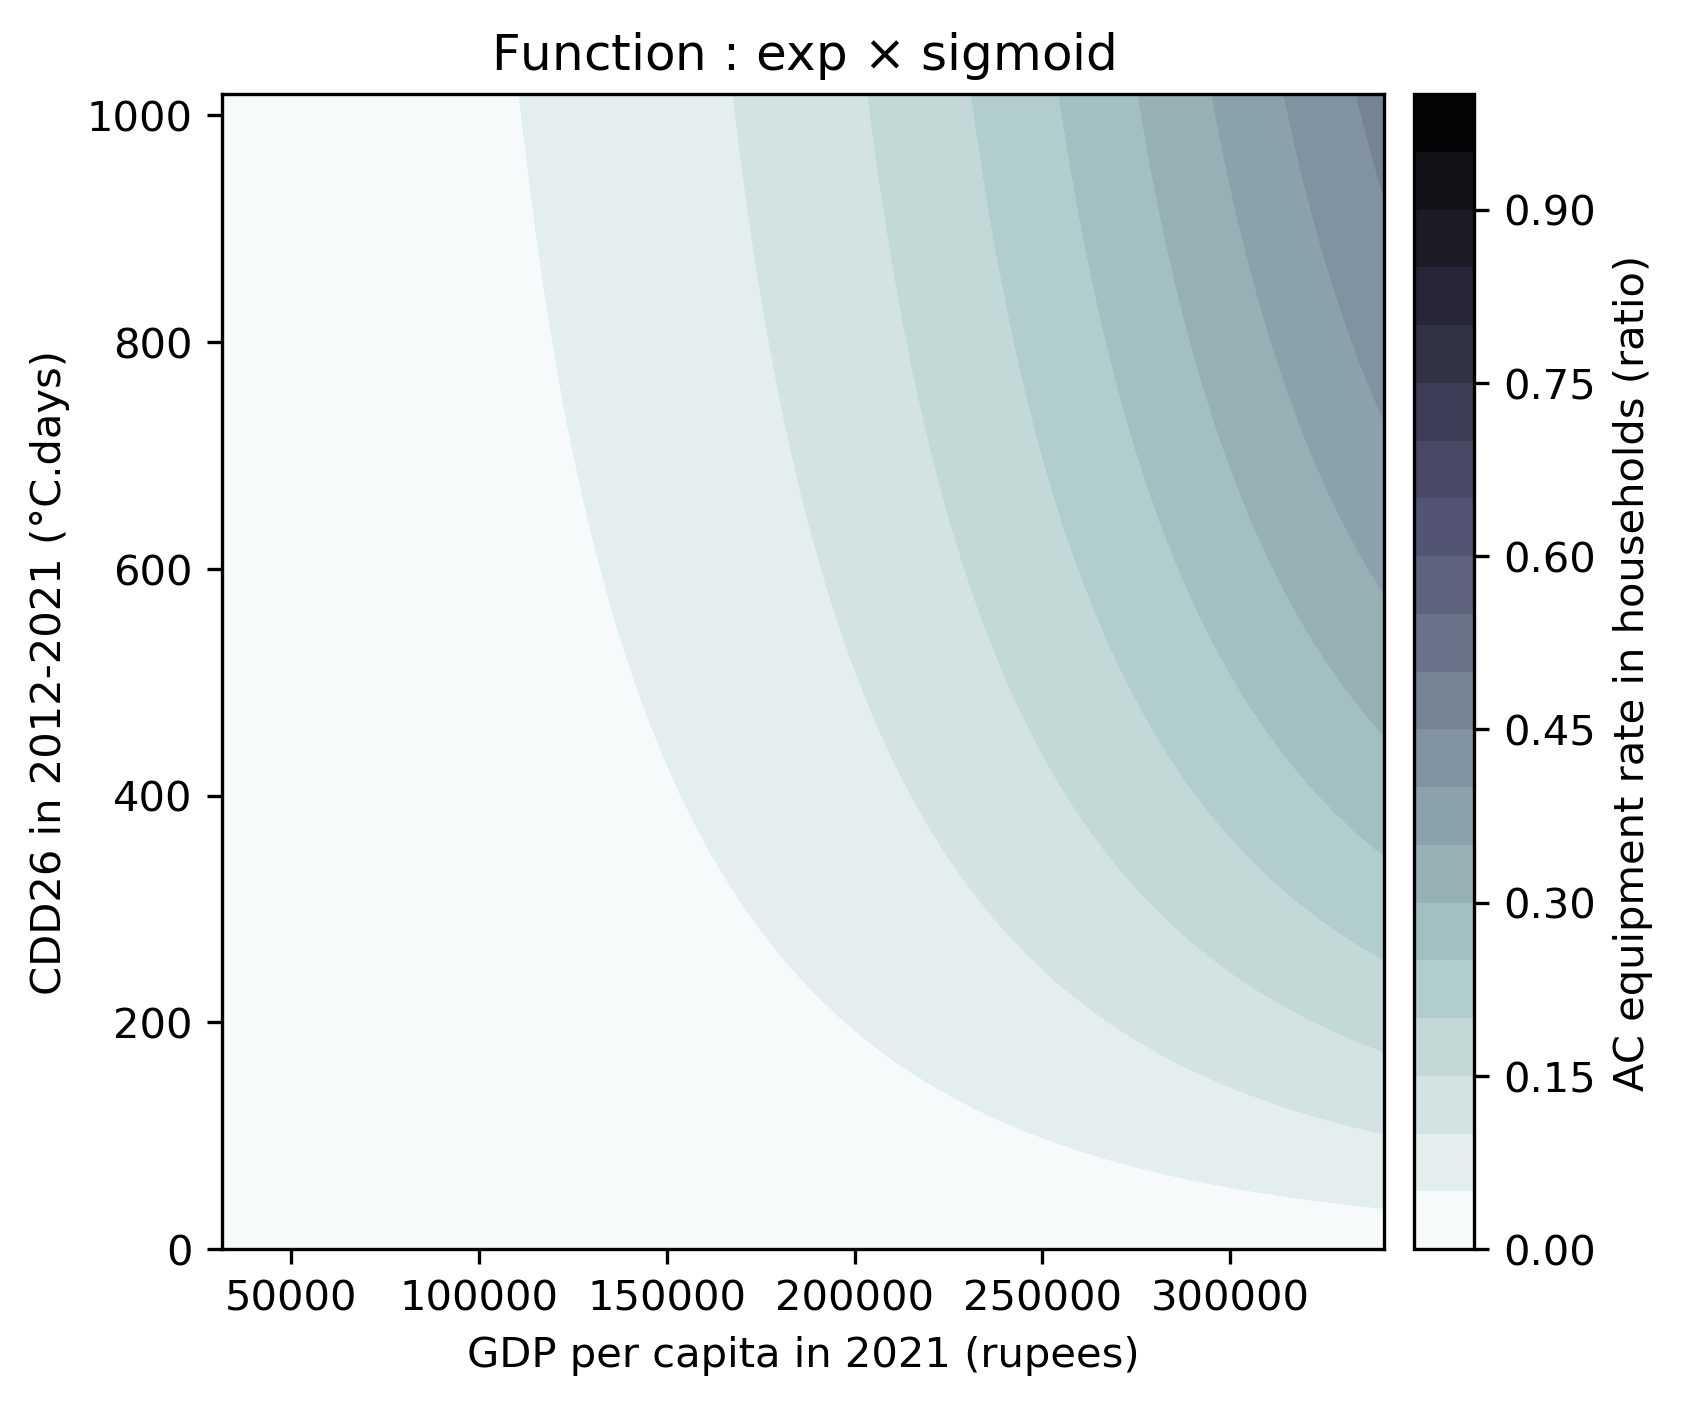
\includegraphics[width=0.38\columnwidth]{figures/cdd26_exp_sigmoid_2dplot.png}
   \caption{\label{fig:es} Résultats de modélisation. De haut en bas, CDD à seuils de 18, 21, 23 et \SI{26}{\celsius}.}
\end{figure}

\clearpage 
\subsection{Modèle $\mathrm{S-S}$}
\begin{figure}[ht]
   \centering
   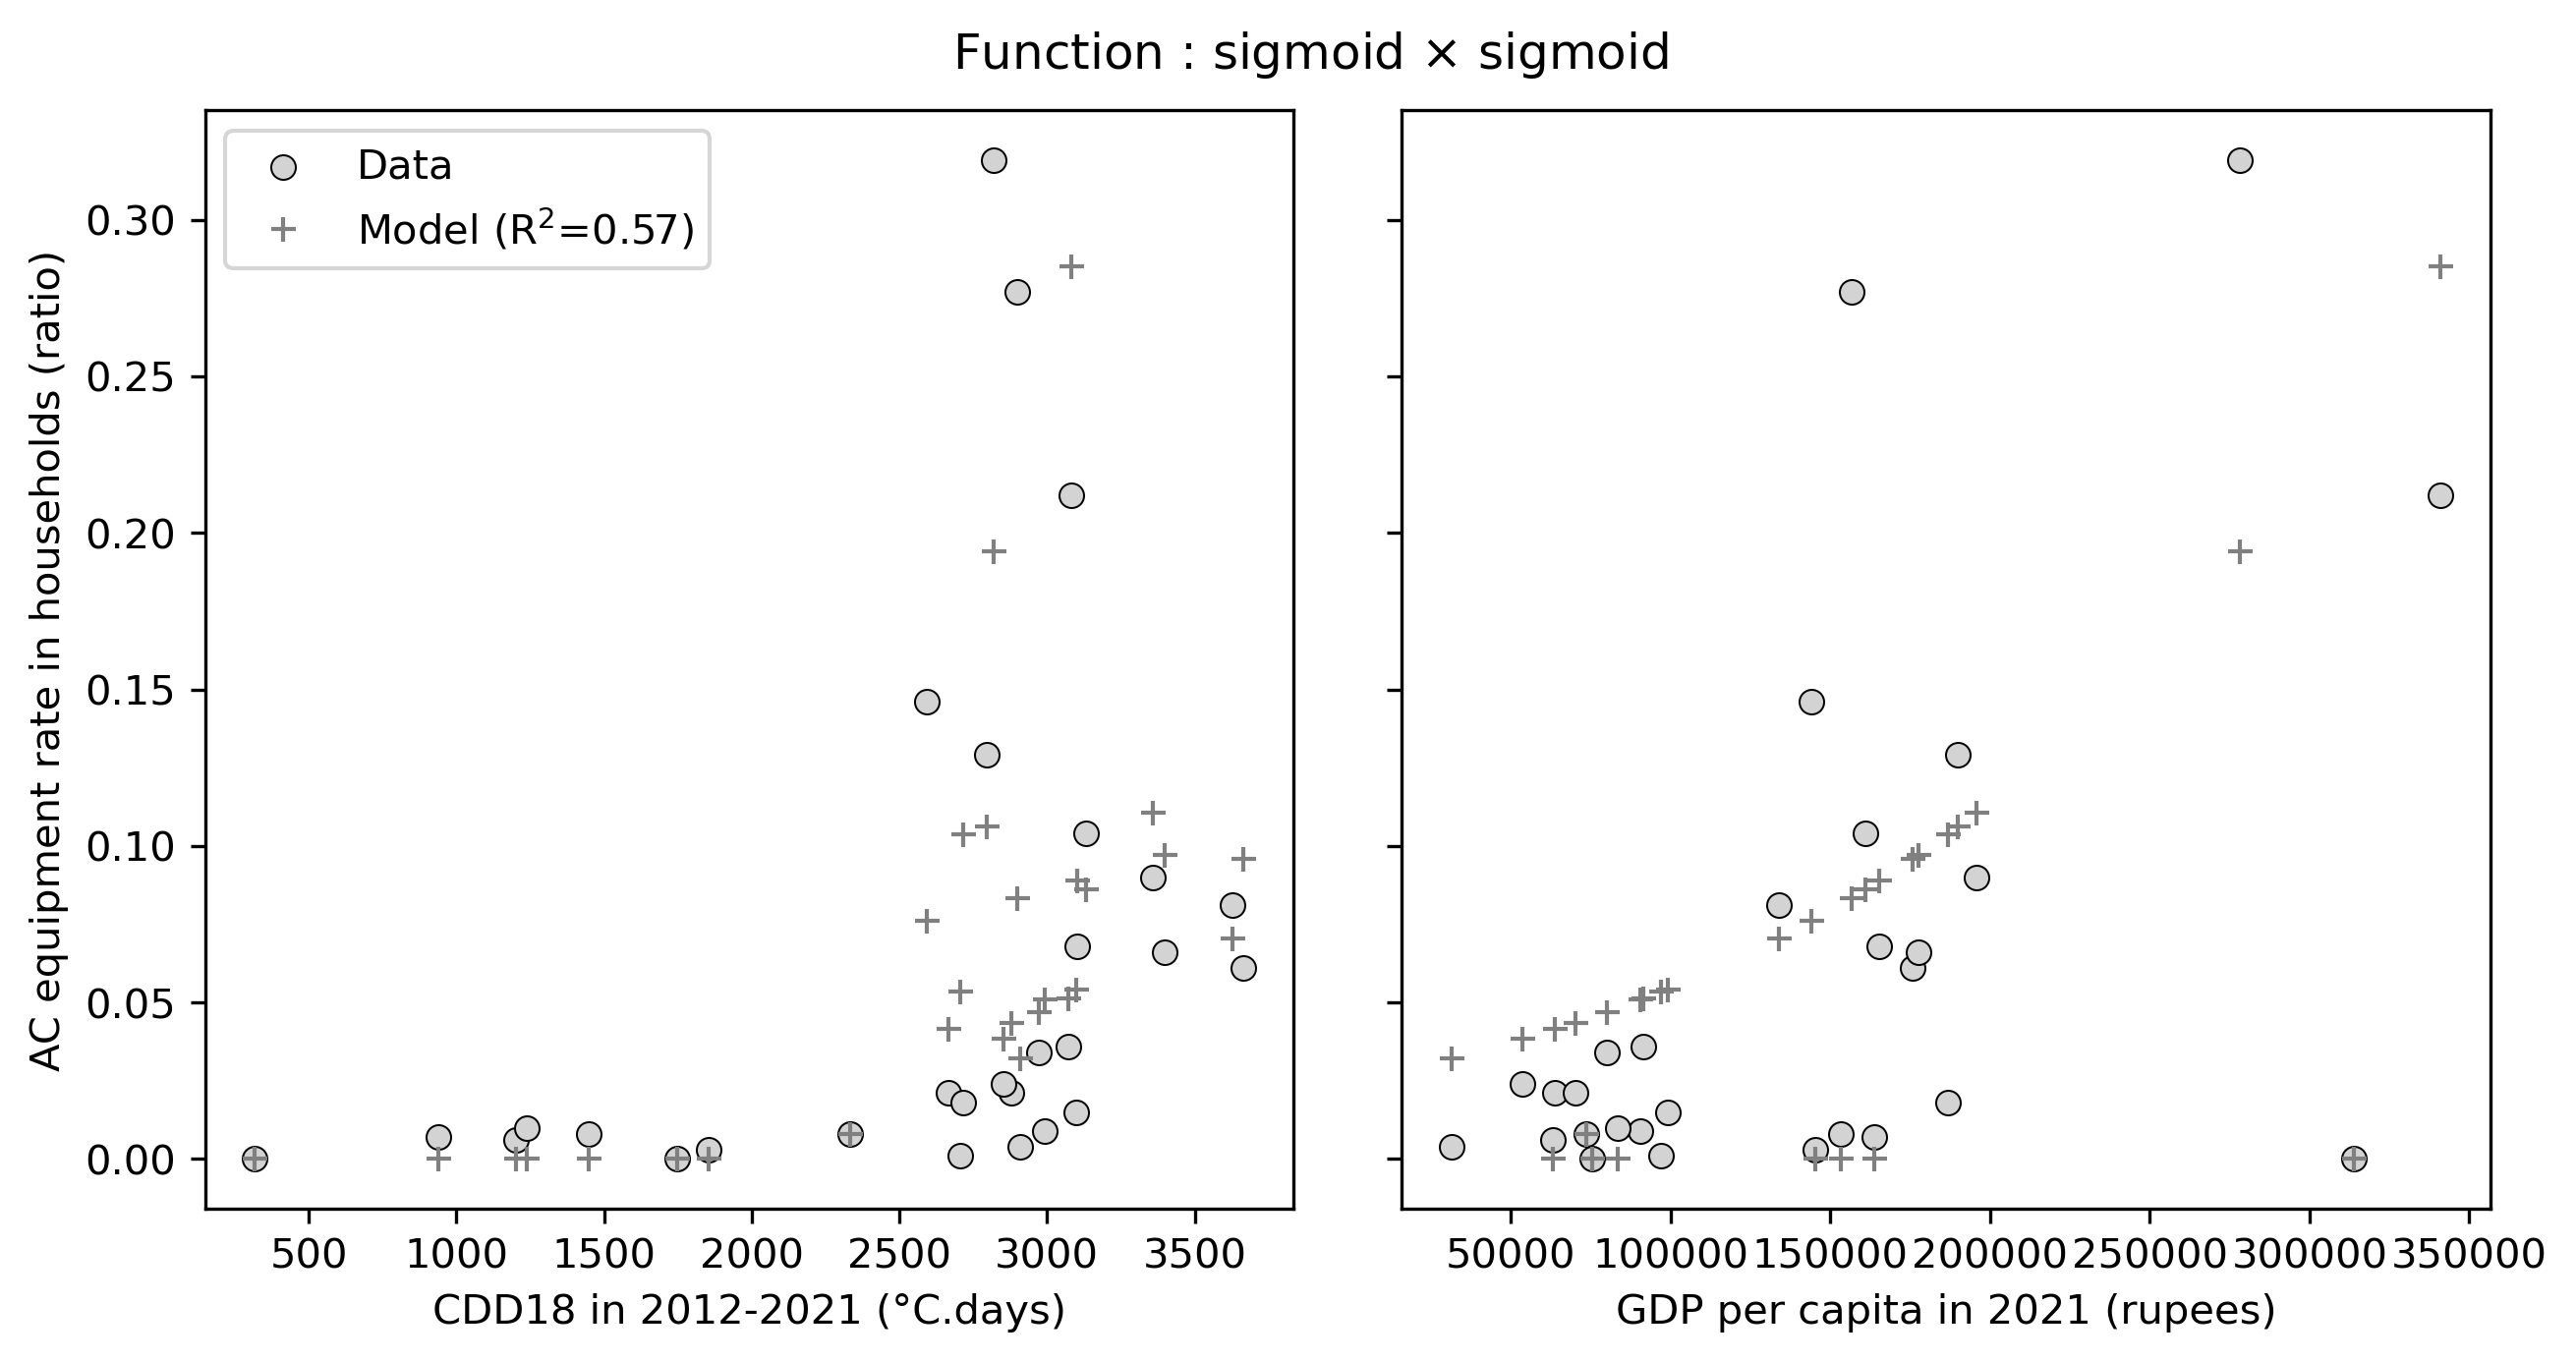
\includegraphics[width=0.6\columnwidth]{figures/cdd18_sigmoid_sigmoid_scatter.png}
   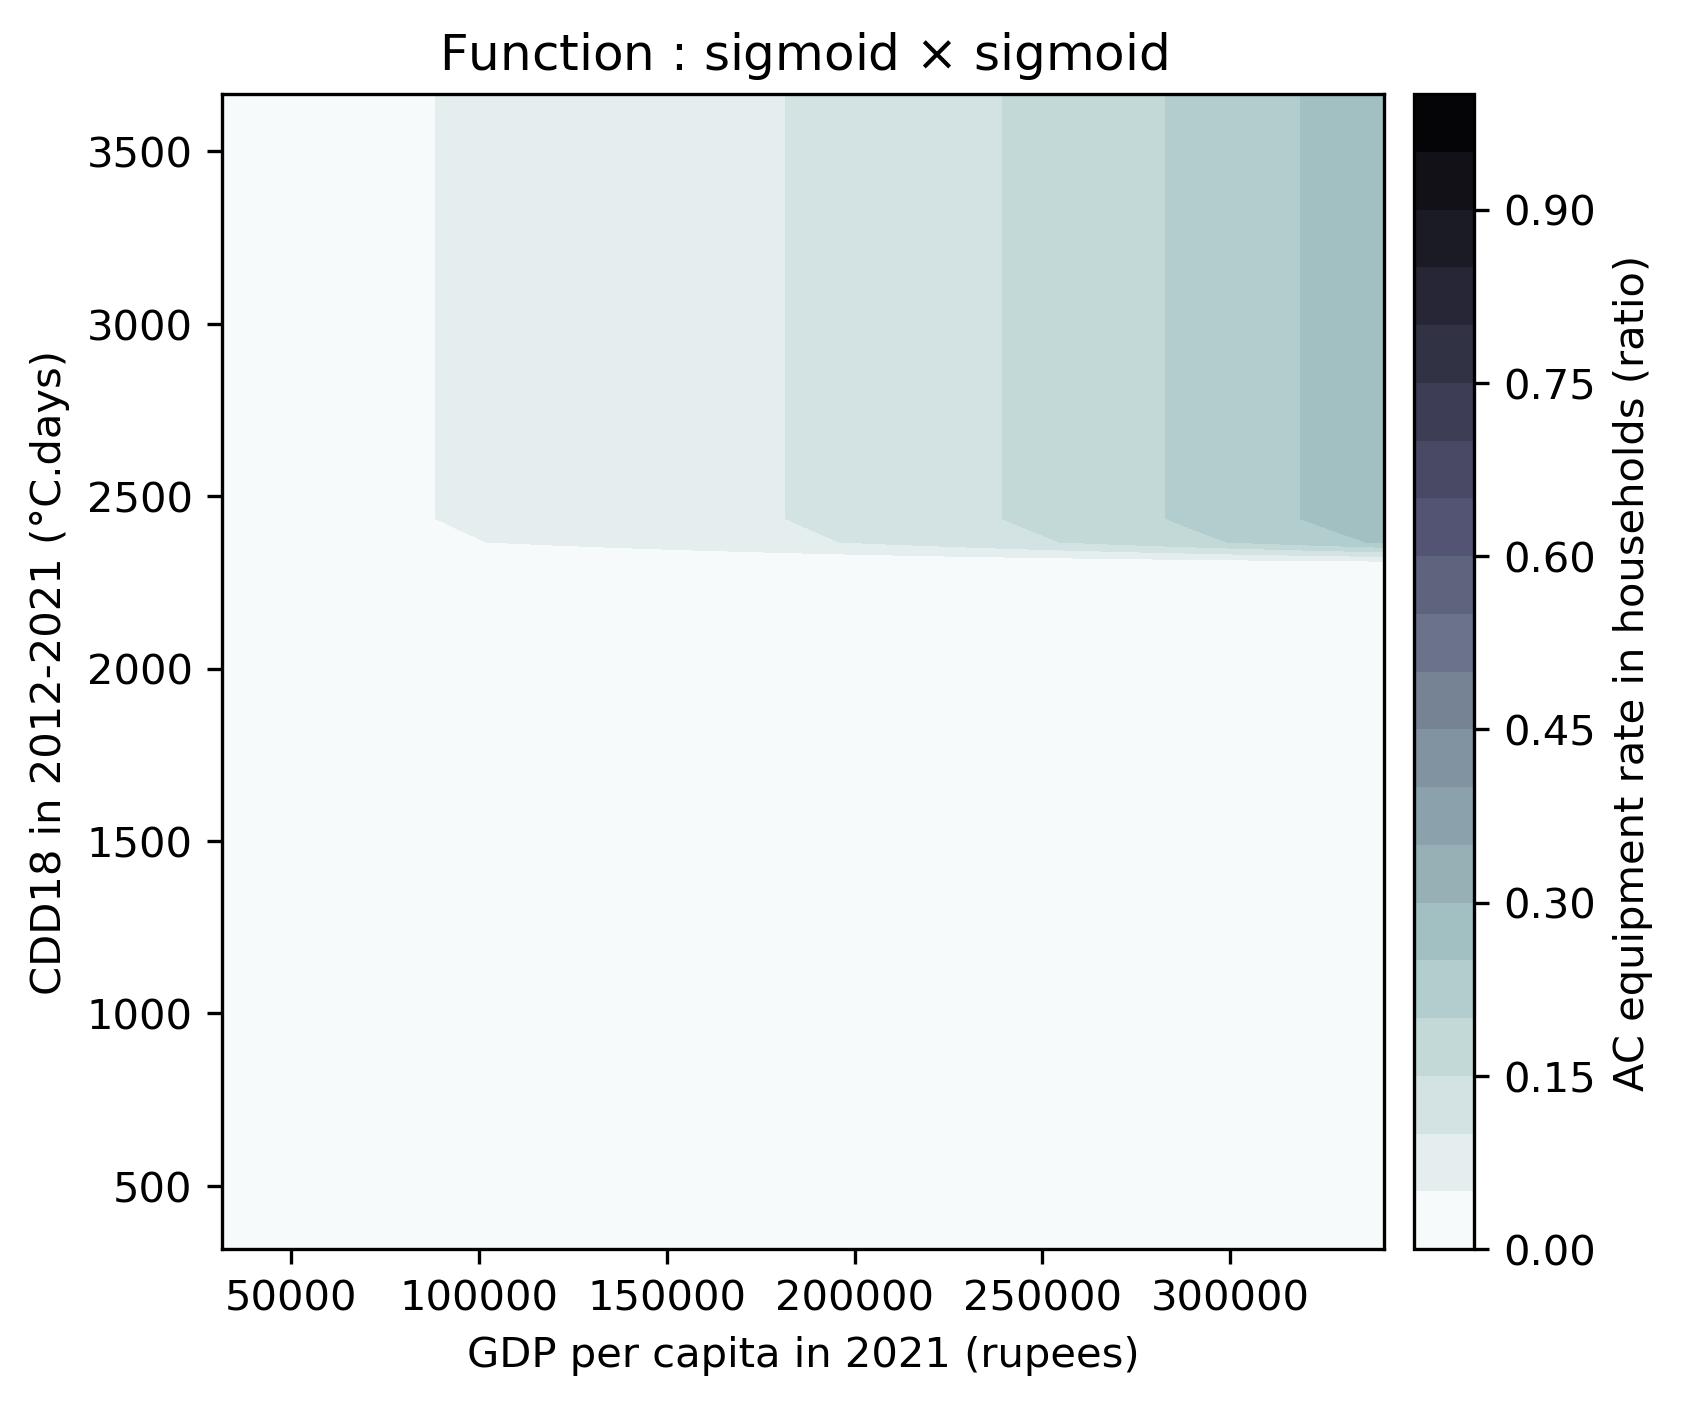
\includegraphics[width=0.38\columnwidth]{figures/cdd18_sigmoid_sigmoid_2dplot.png}

   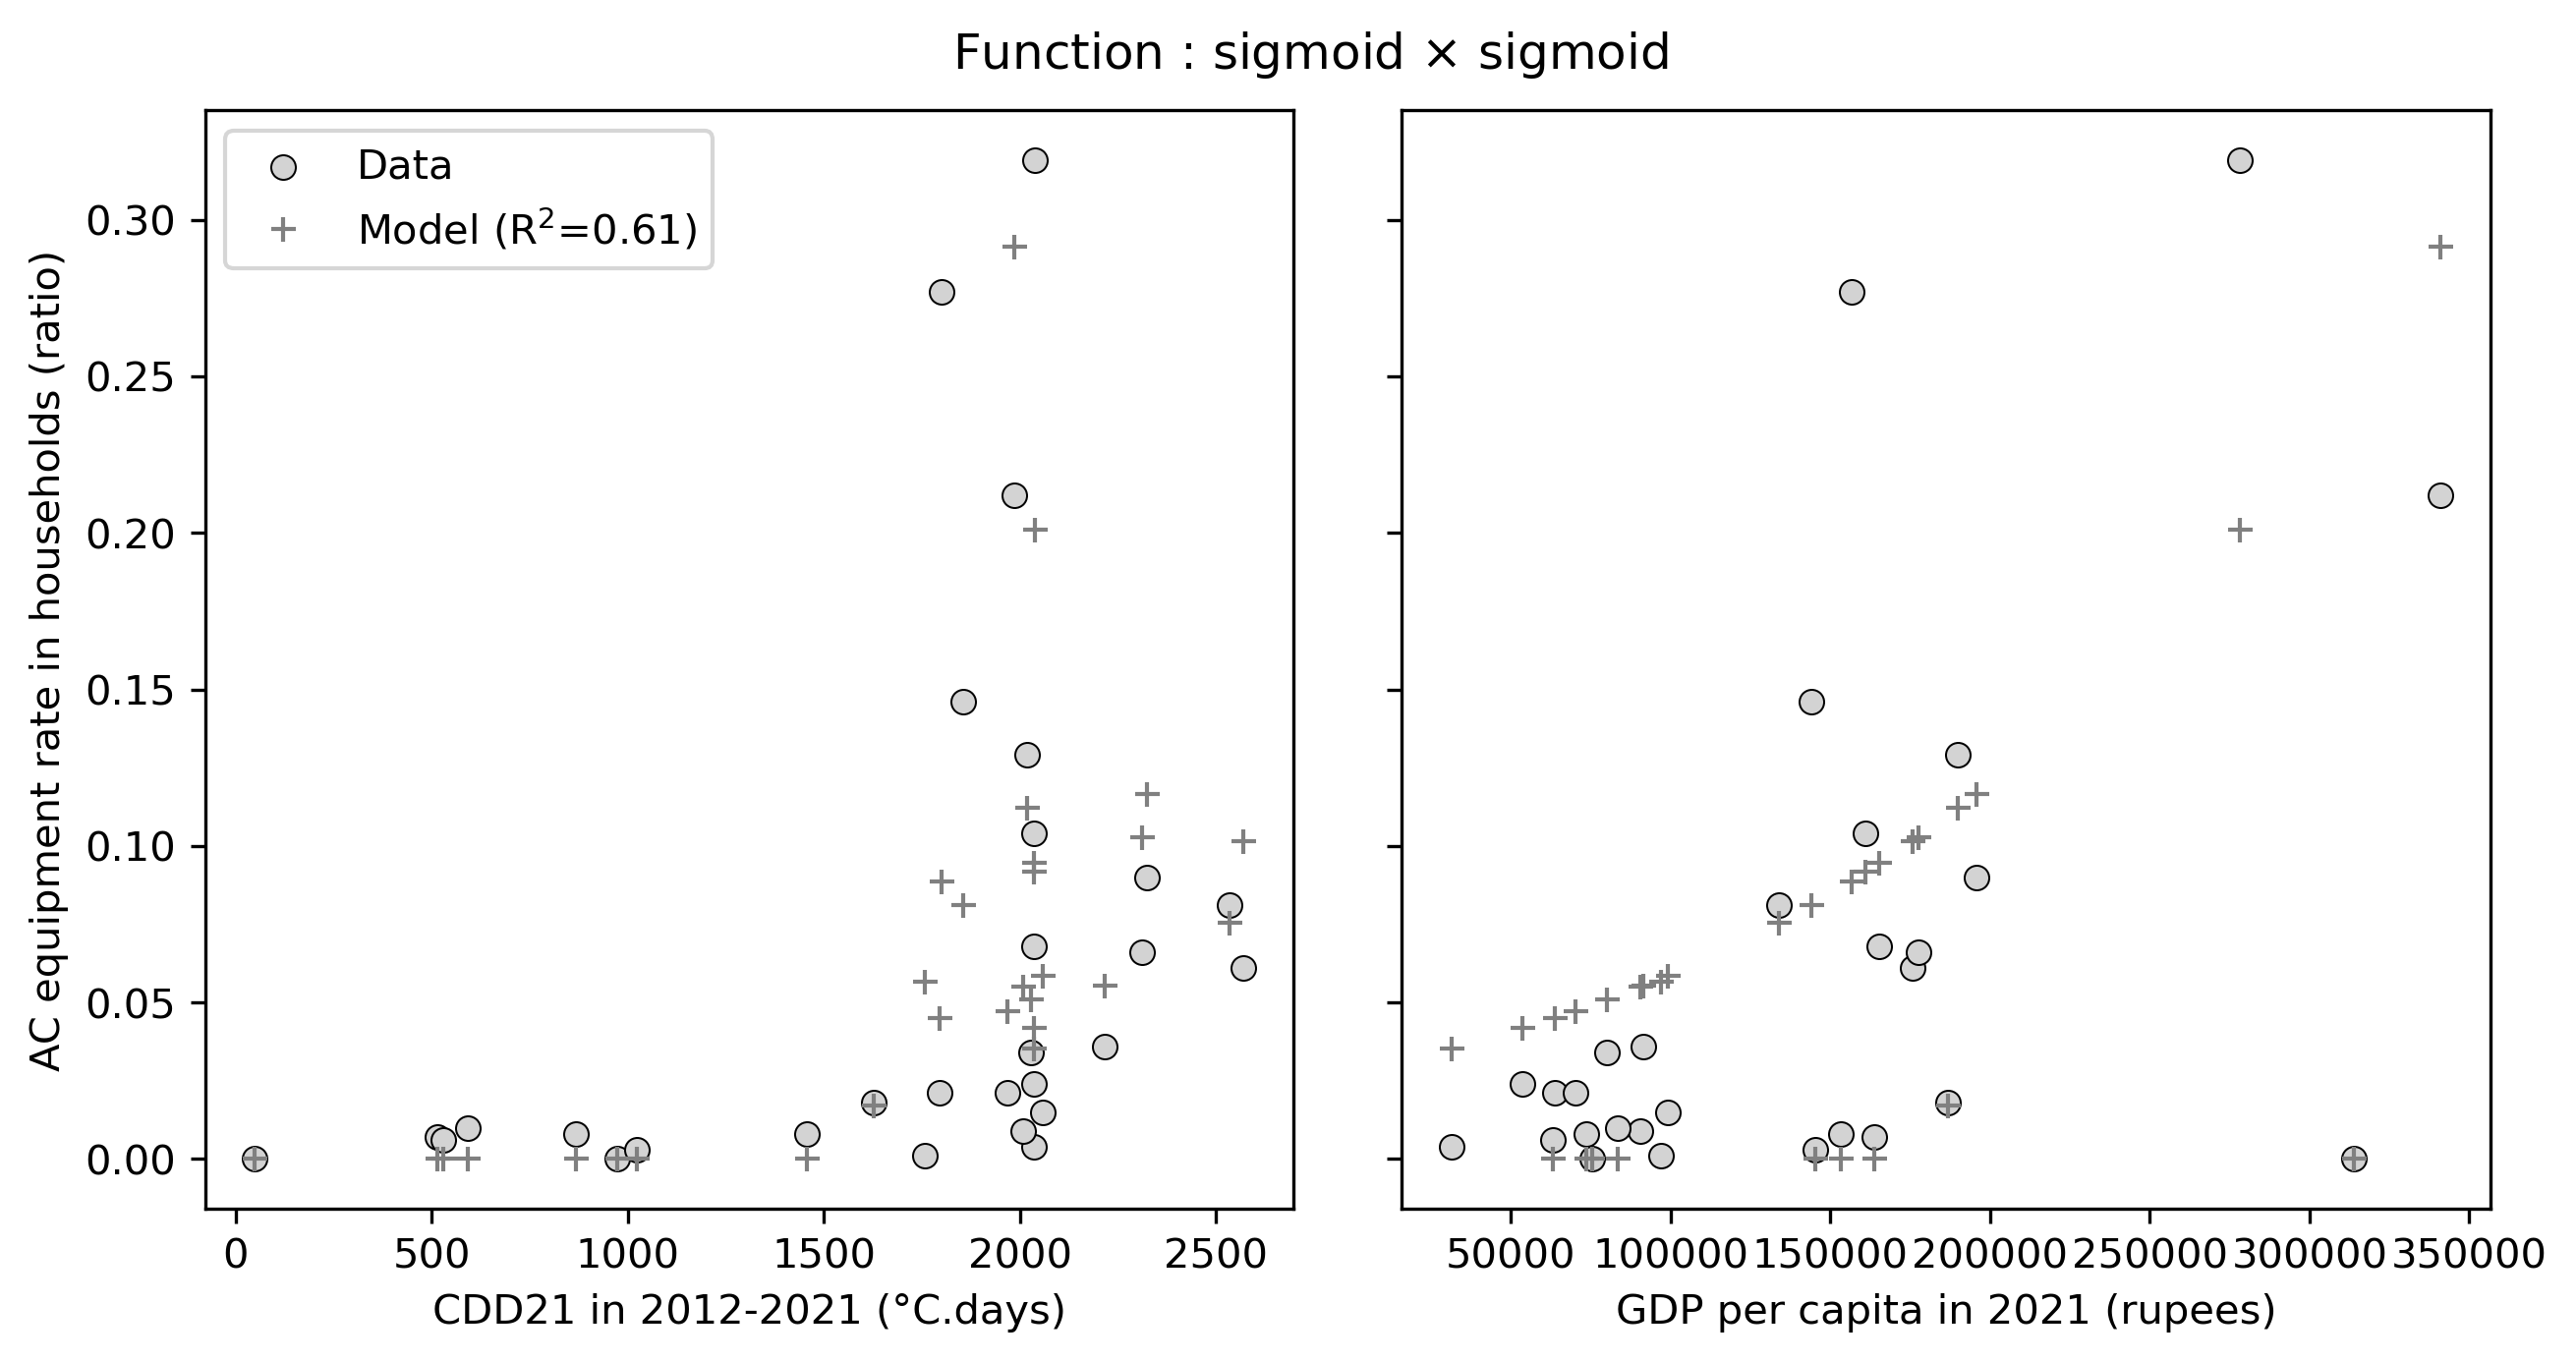
\includegraphics[width=0.6\columnwidth]{figures/cdd21_sigmoid_sigmoid_scatter.png}
   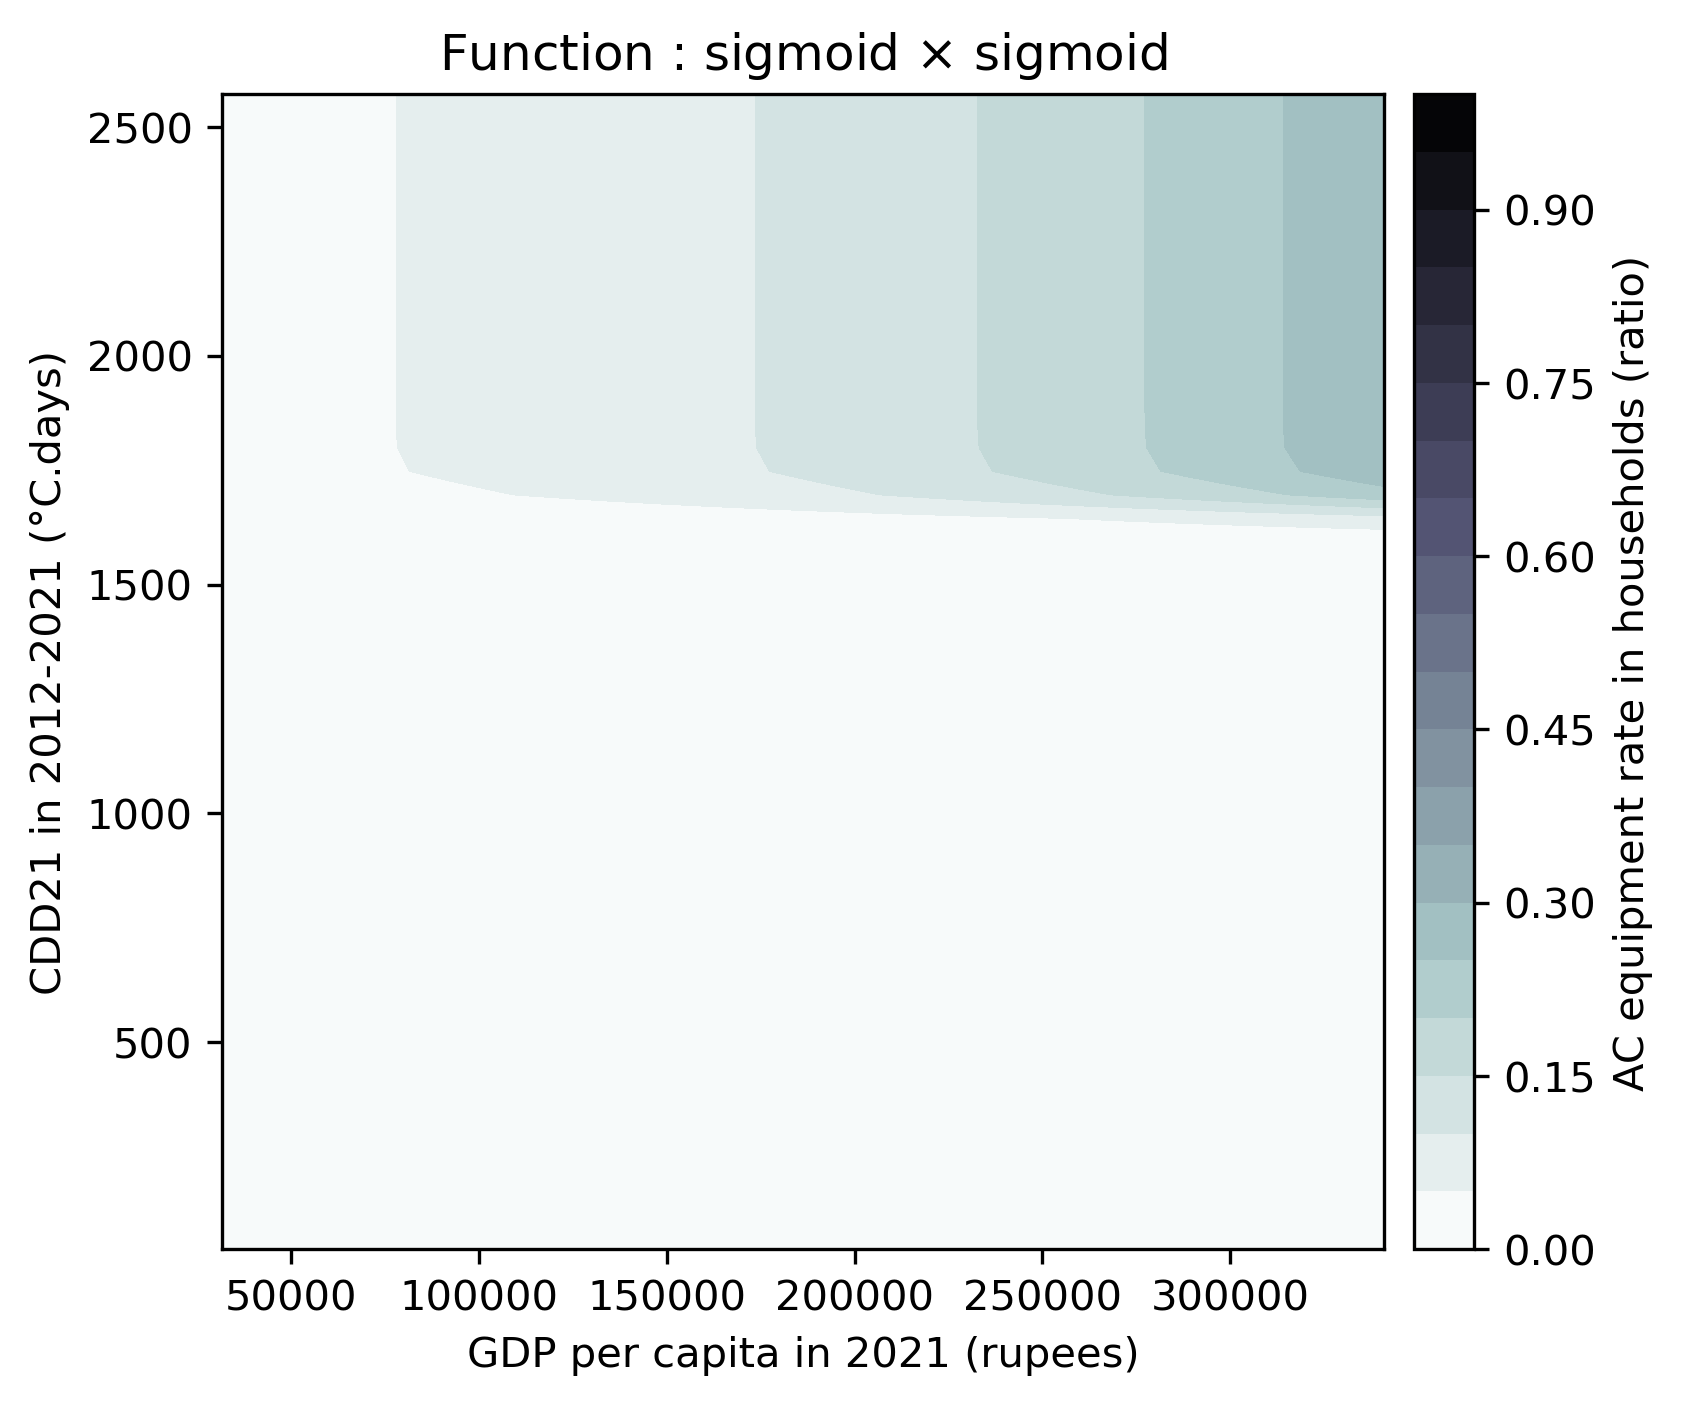
\includegraphics[width=0.38\columnwidth]{figures/cdd21_sigmoid_sigmoid_2dplot.png}

   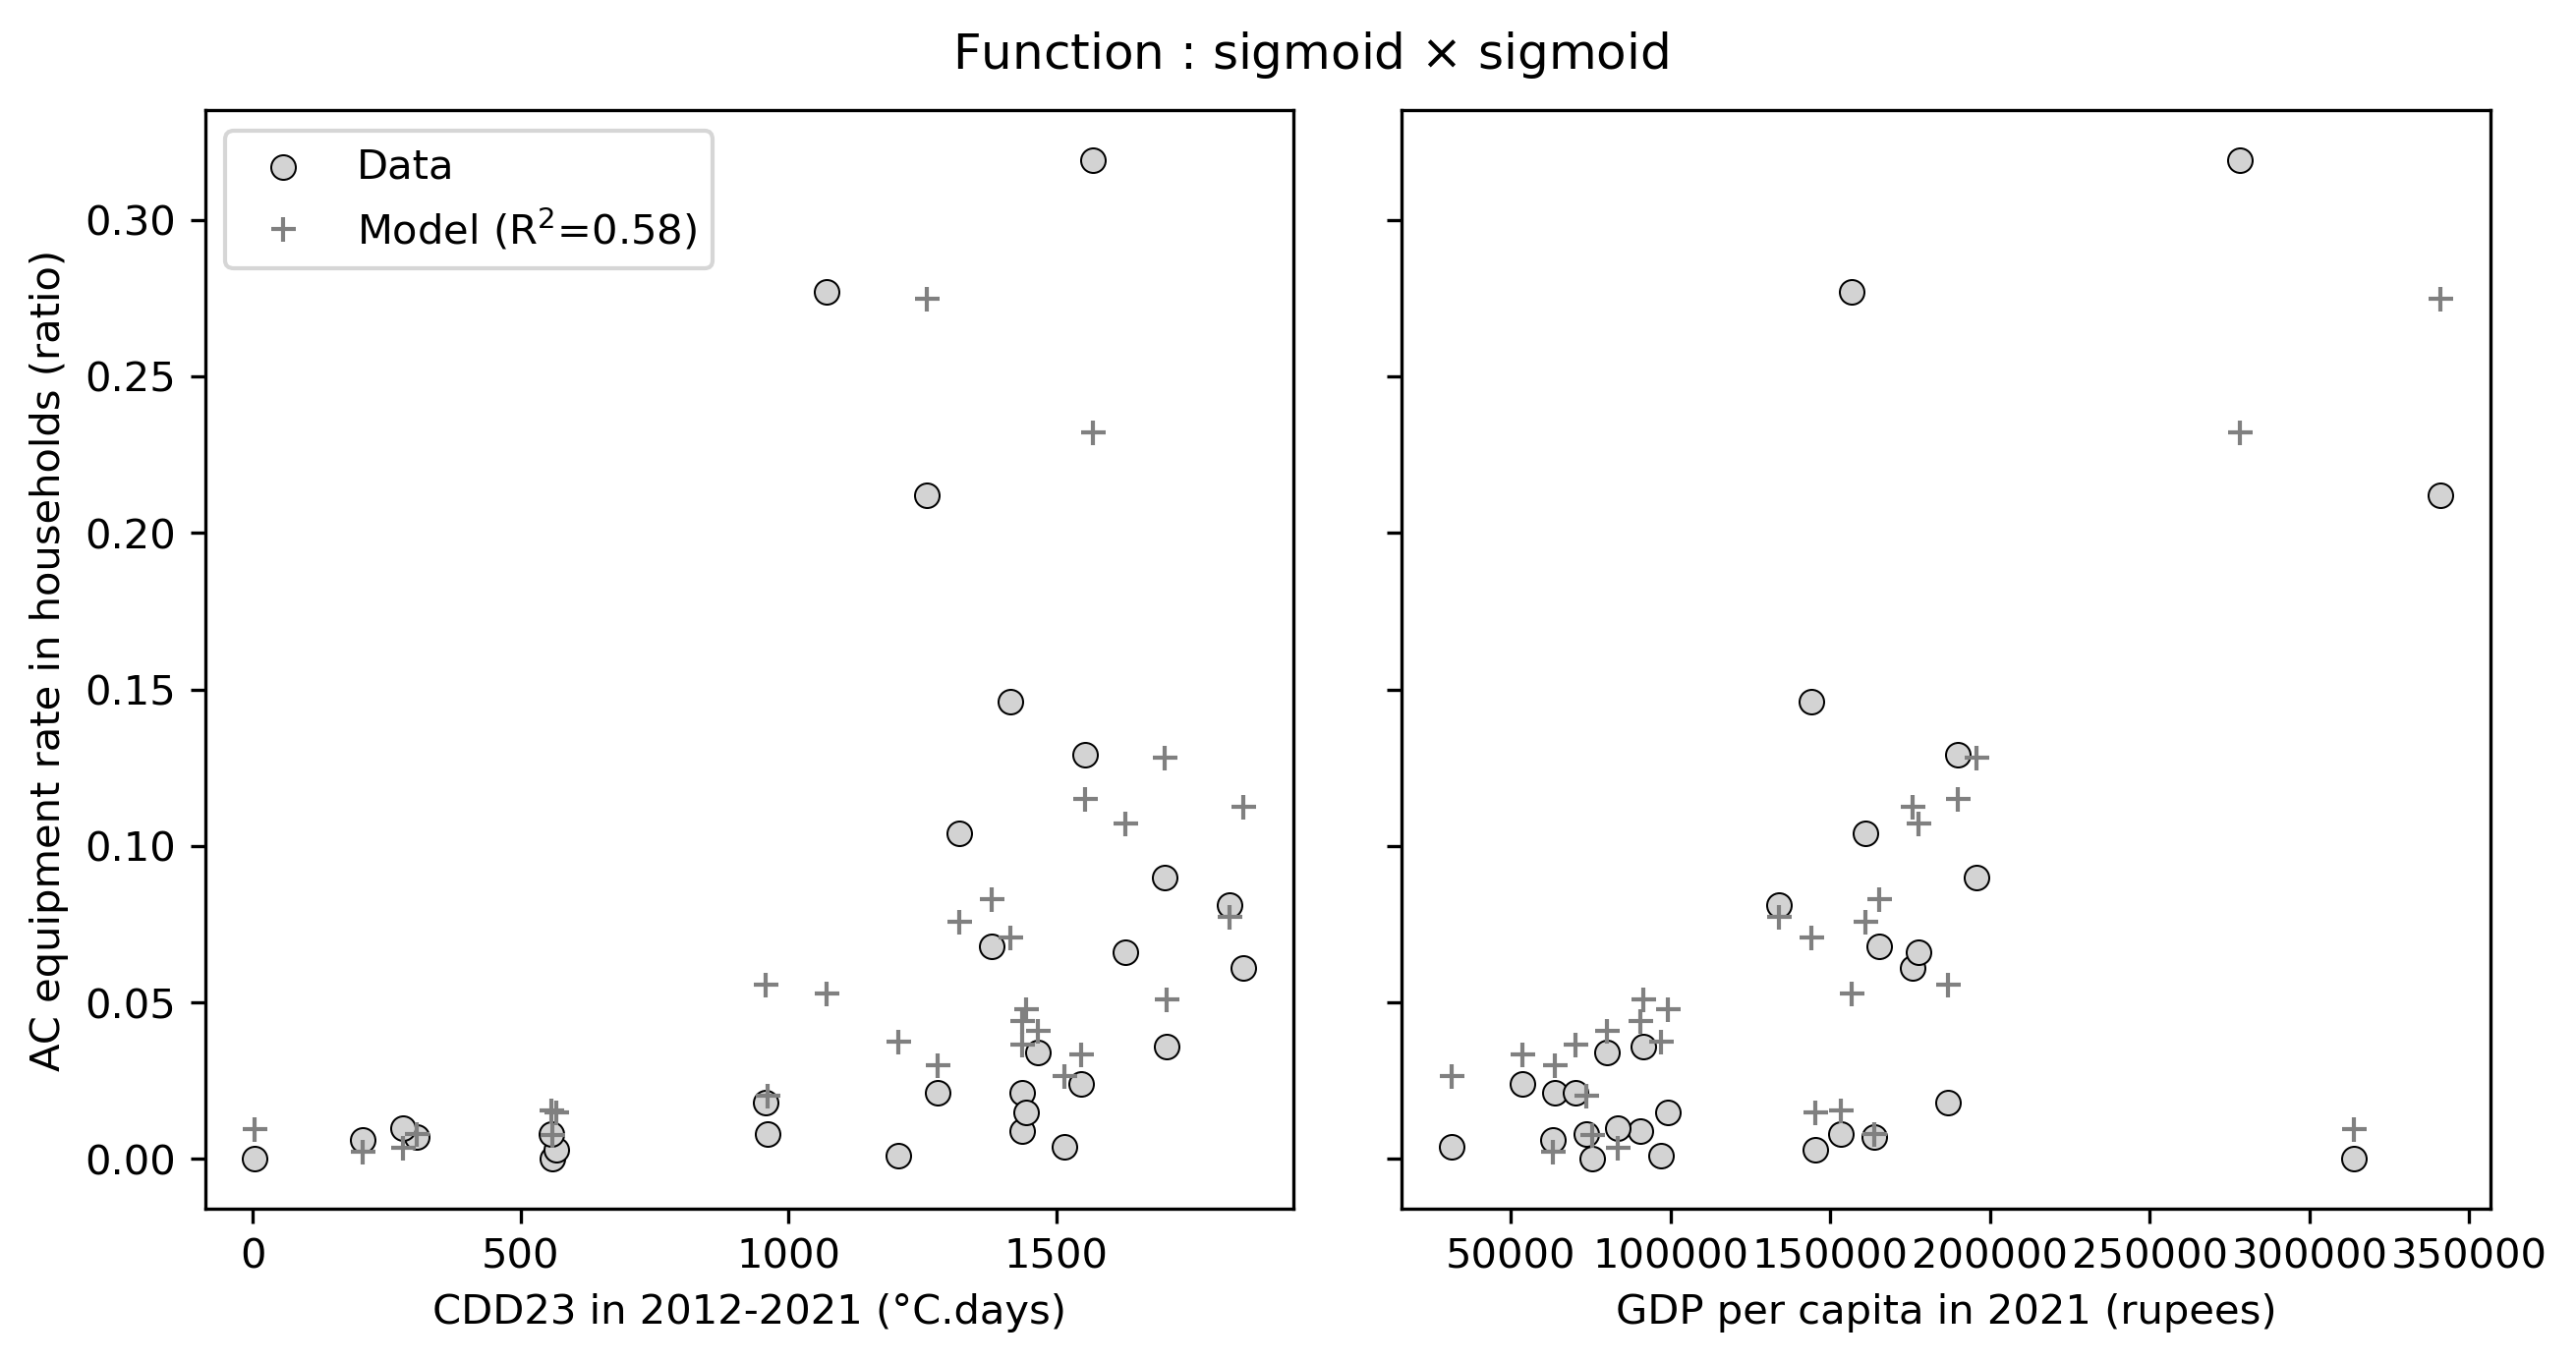
\includegraphics[width=0.6\columnwidth]{figures/cdd23_sigmoid_sigmoid_scatter.png}
   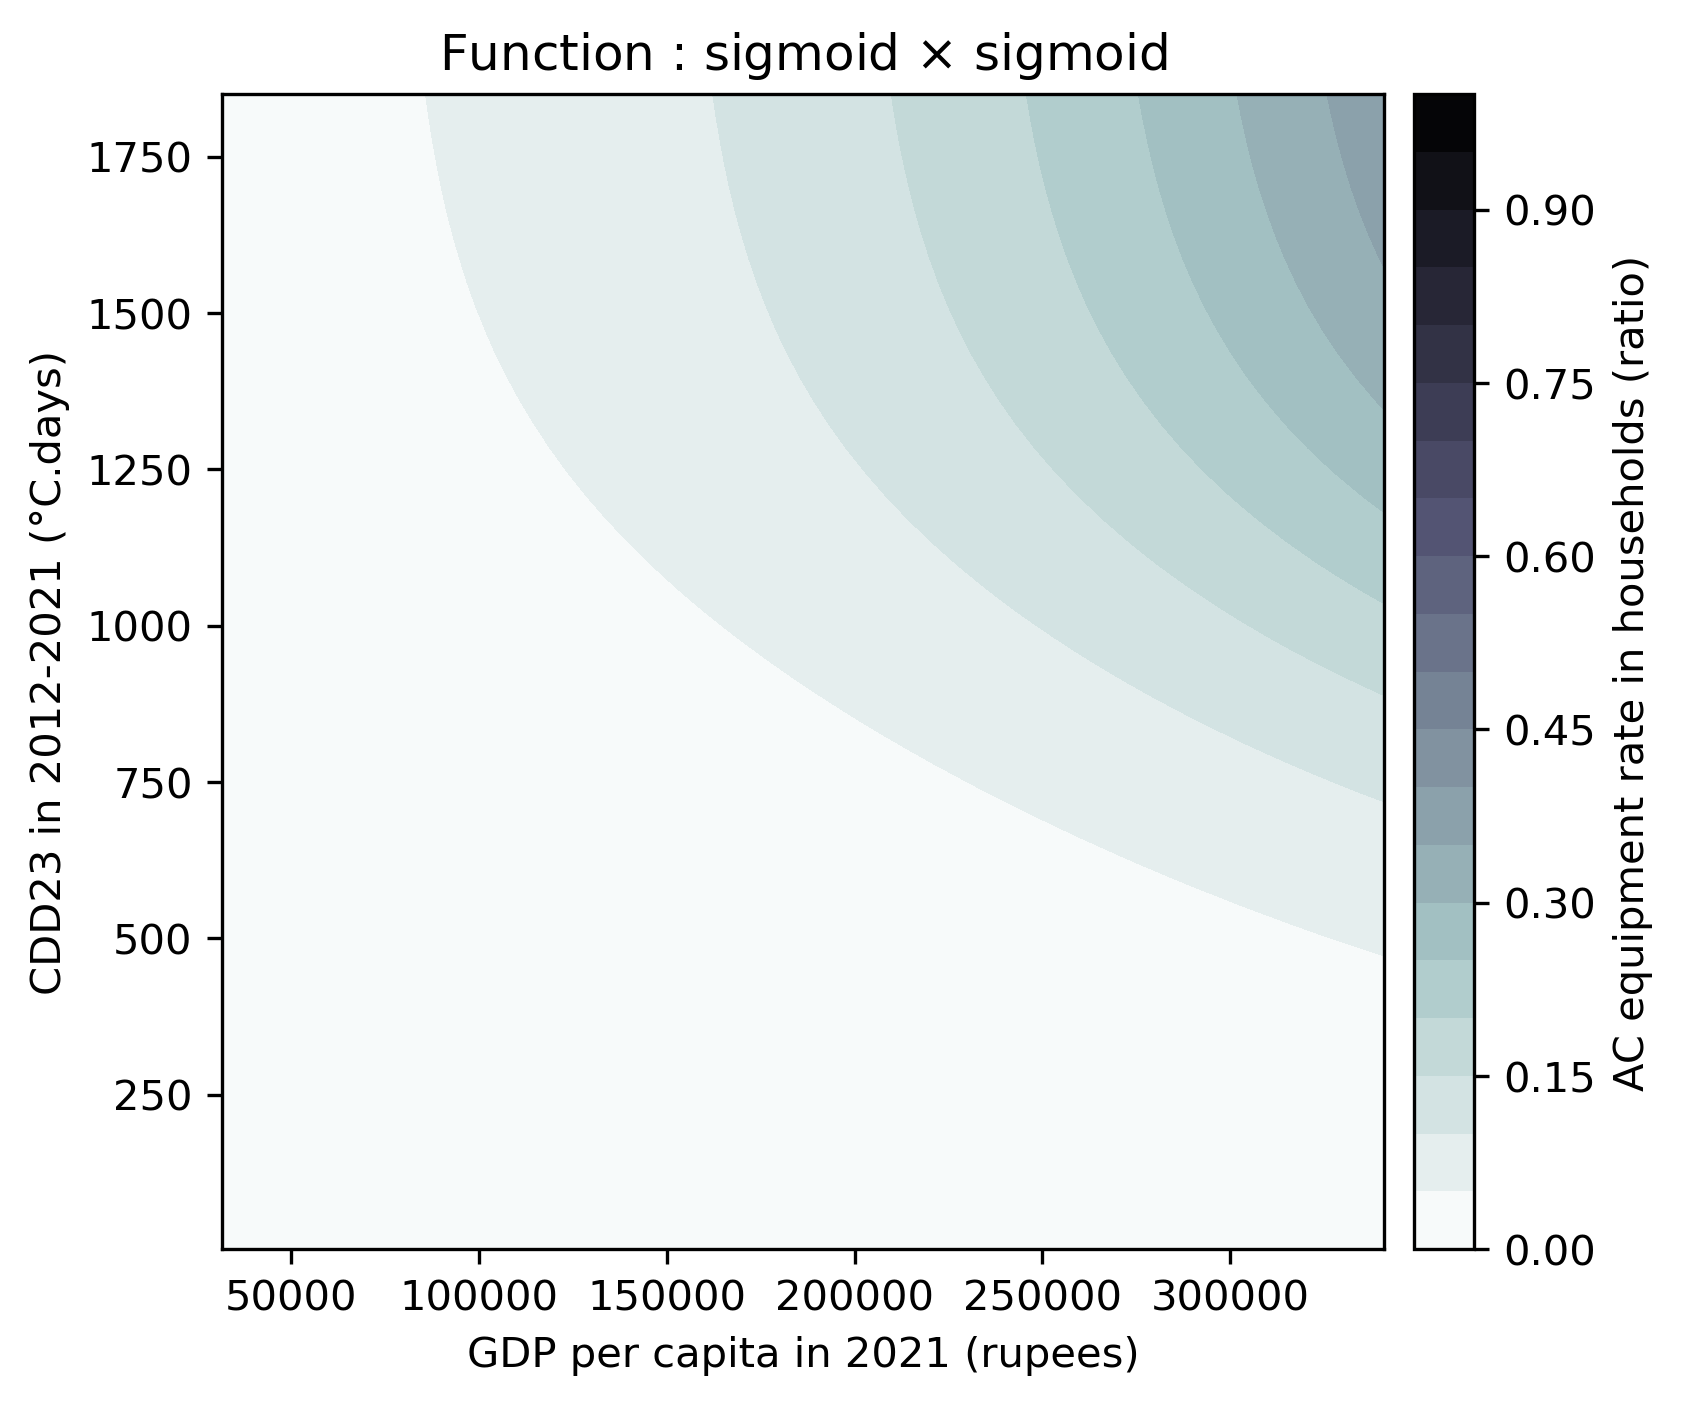
\includegraphics[width=0.38\columnwidth]{figures/cdd23_sigmoid_sigmoid_2dplot.png}

   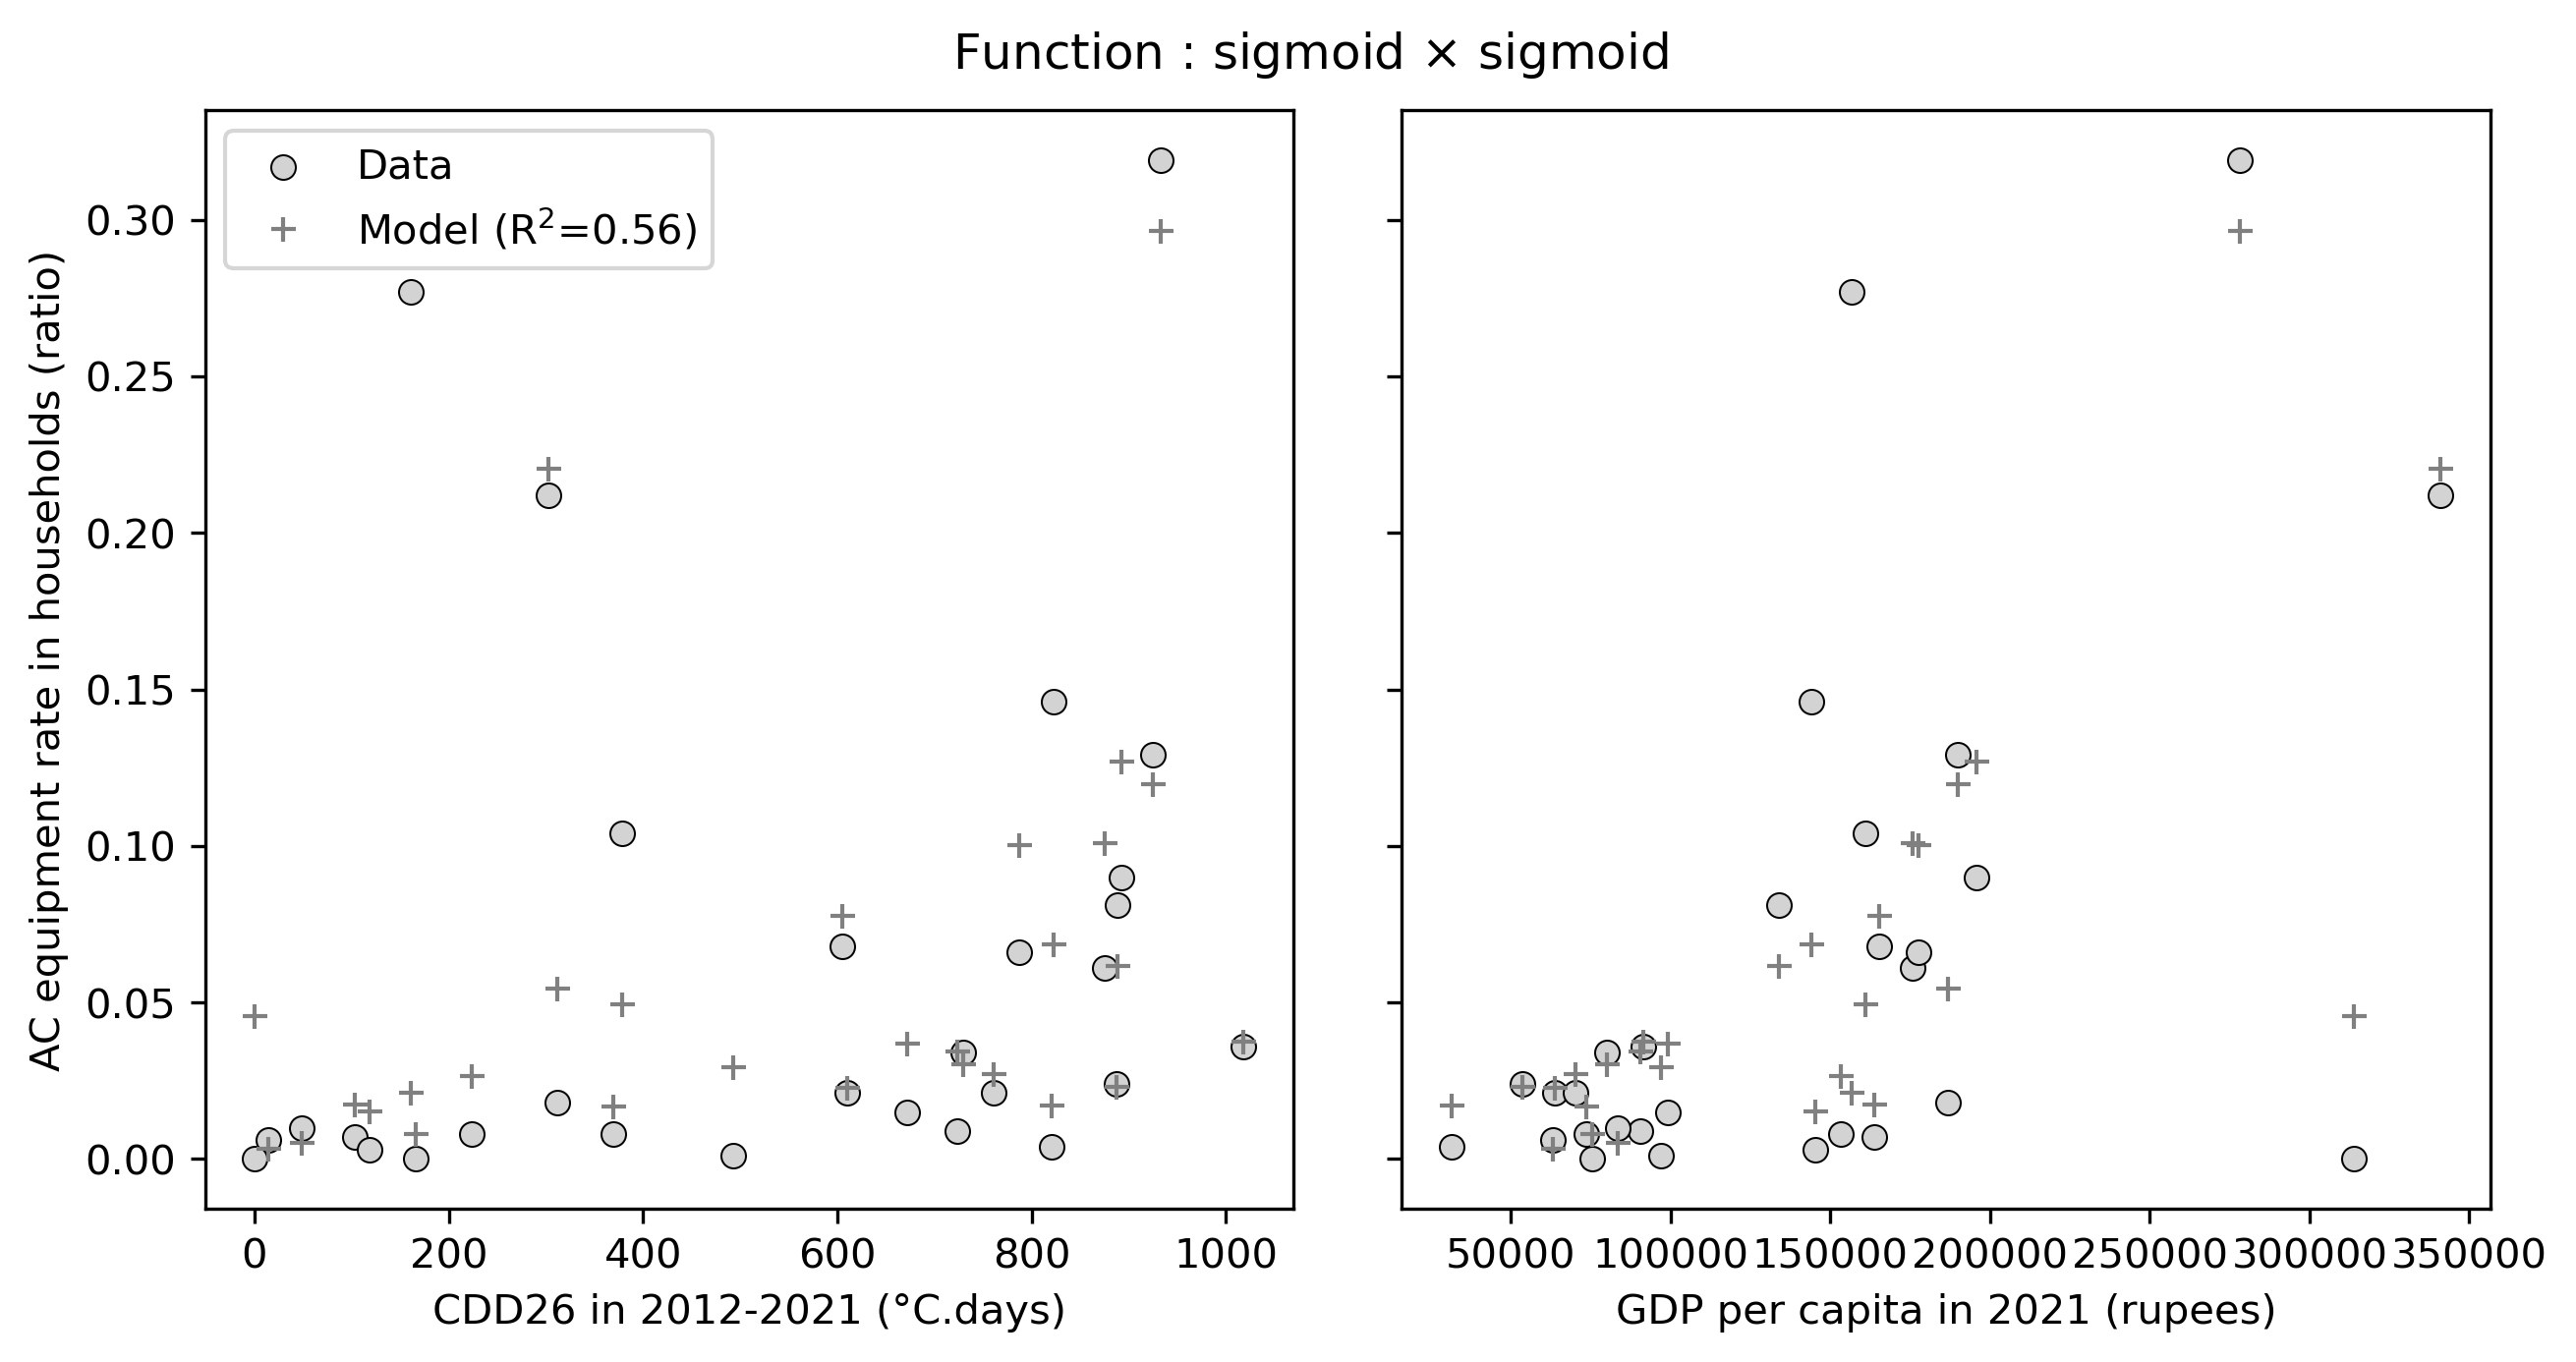
\includegraphics[width=0.6\columnwidth]{figures/cdd26_sigmoid_sigmoid_scatter.png}
   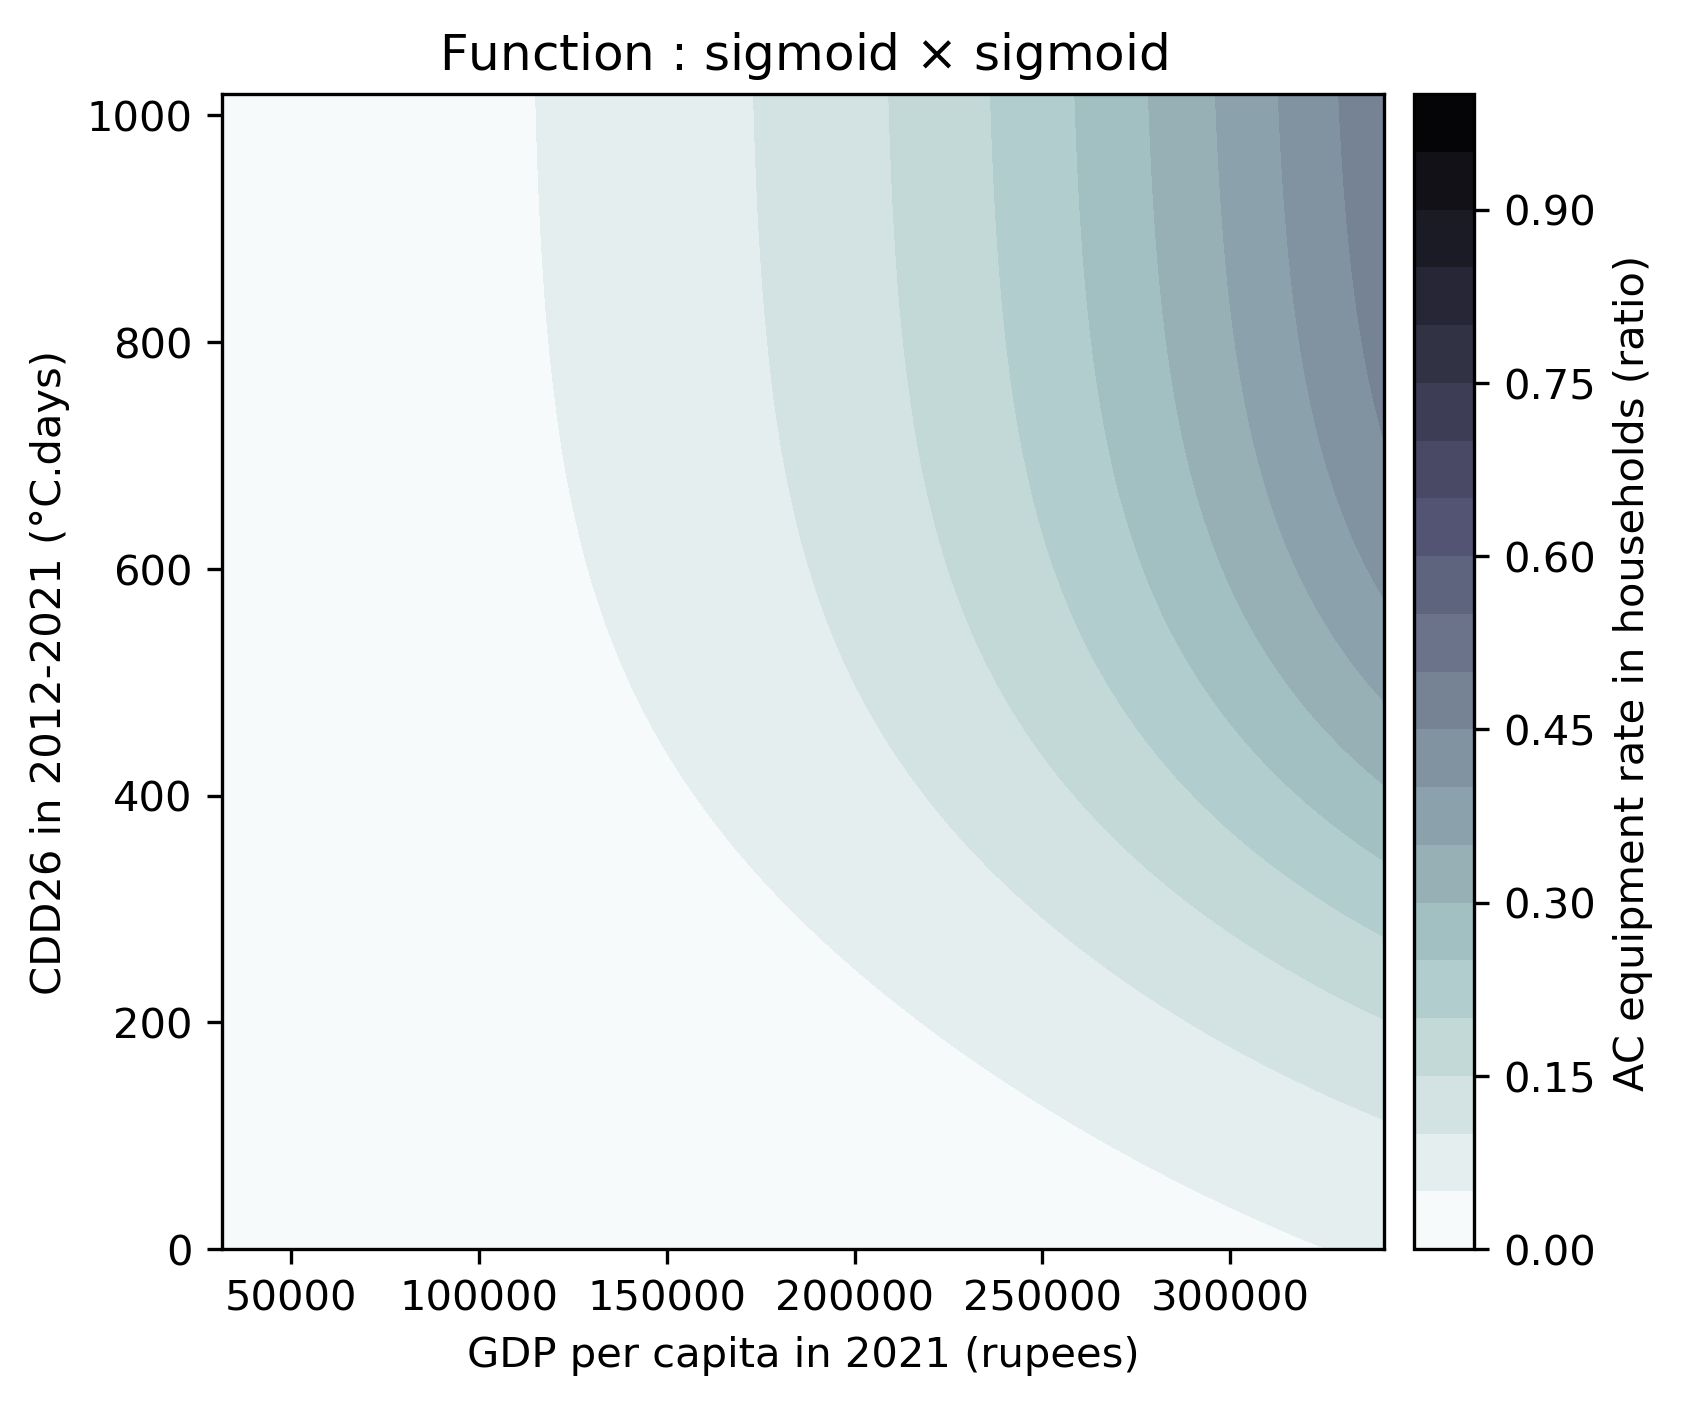
\includegraphics[width=0.38\columnwidth]{figures/cdd26_sigmoid_sigmoid_2dplot.png}
   \caption{\label{fig:ss} Résultats de modélisation. De haut en bas, CDD à seuils de 18, 21, 23 et \SI{26}{\celsius}.}
\end{figure}

\clearpage 
\subsection{Modèle $\mathrm{E-E}$}
\begin{figure}[ht]
   \centering
   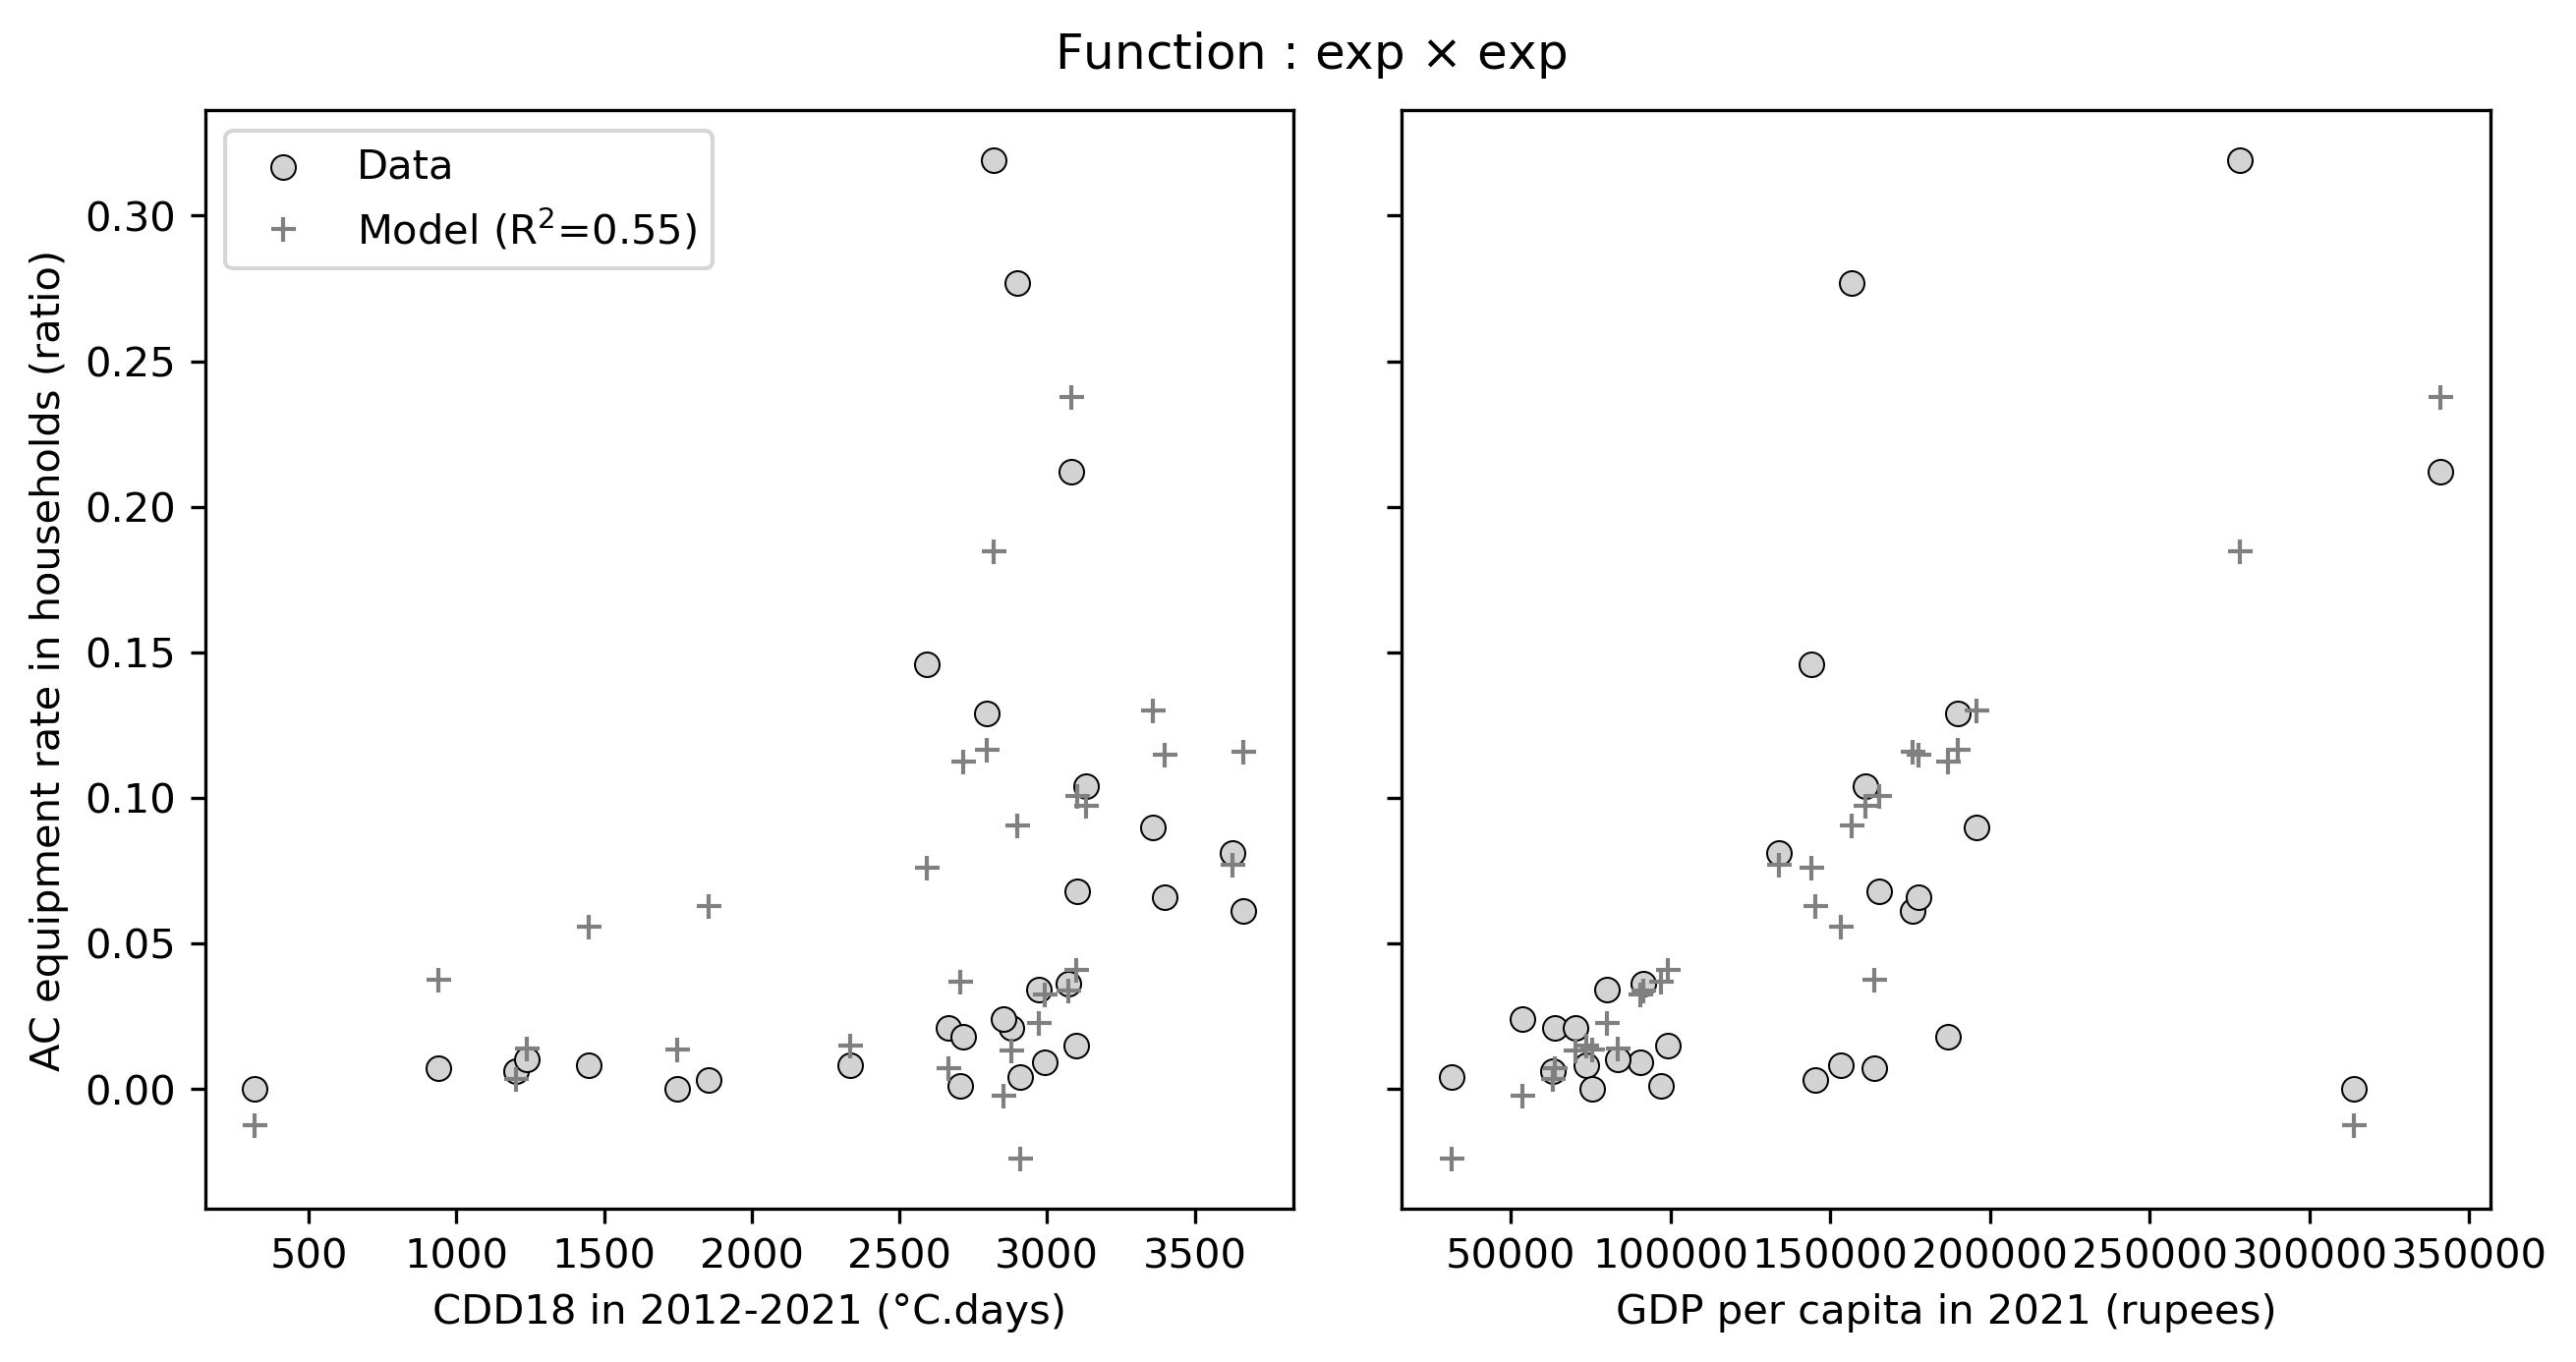
\includegraphics[width=0.6\columnwidth]{figures/cdd18_exp_exp_scatter.png}
   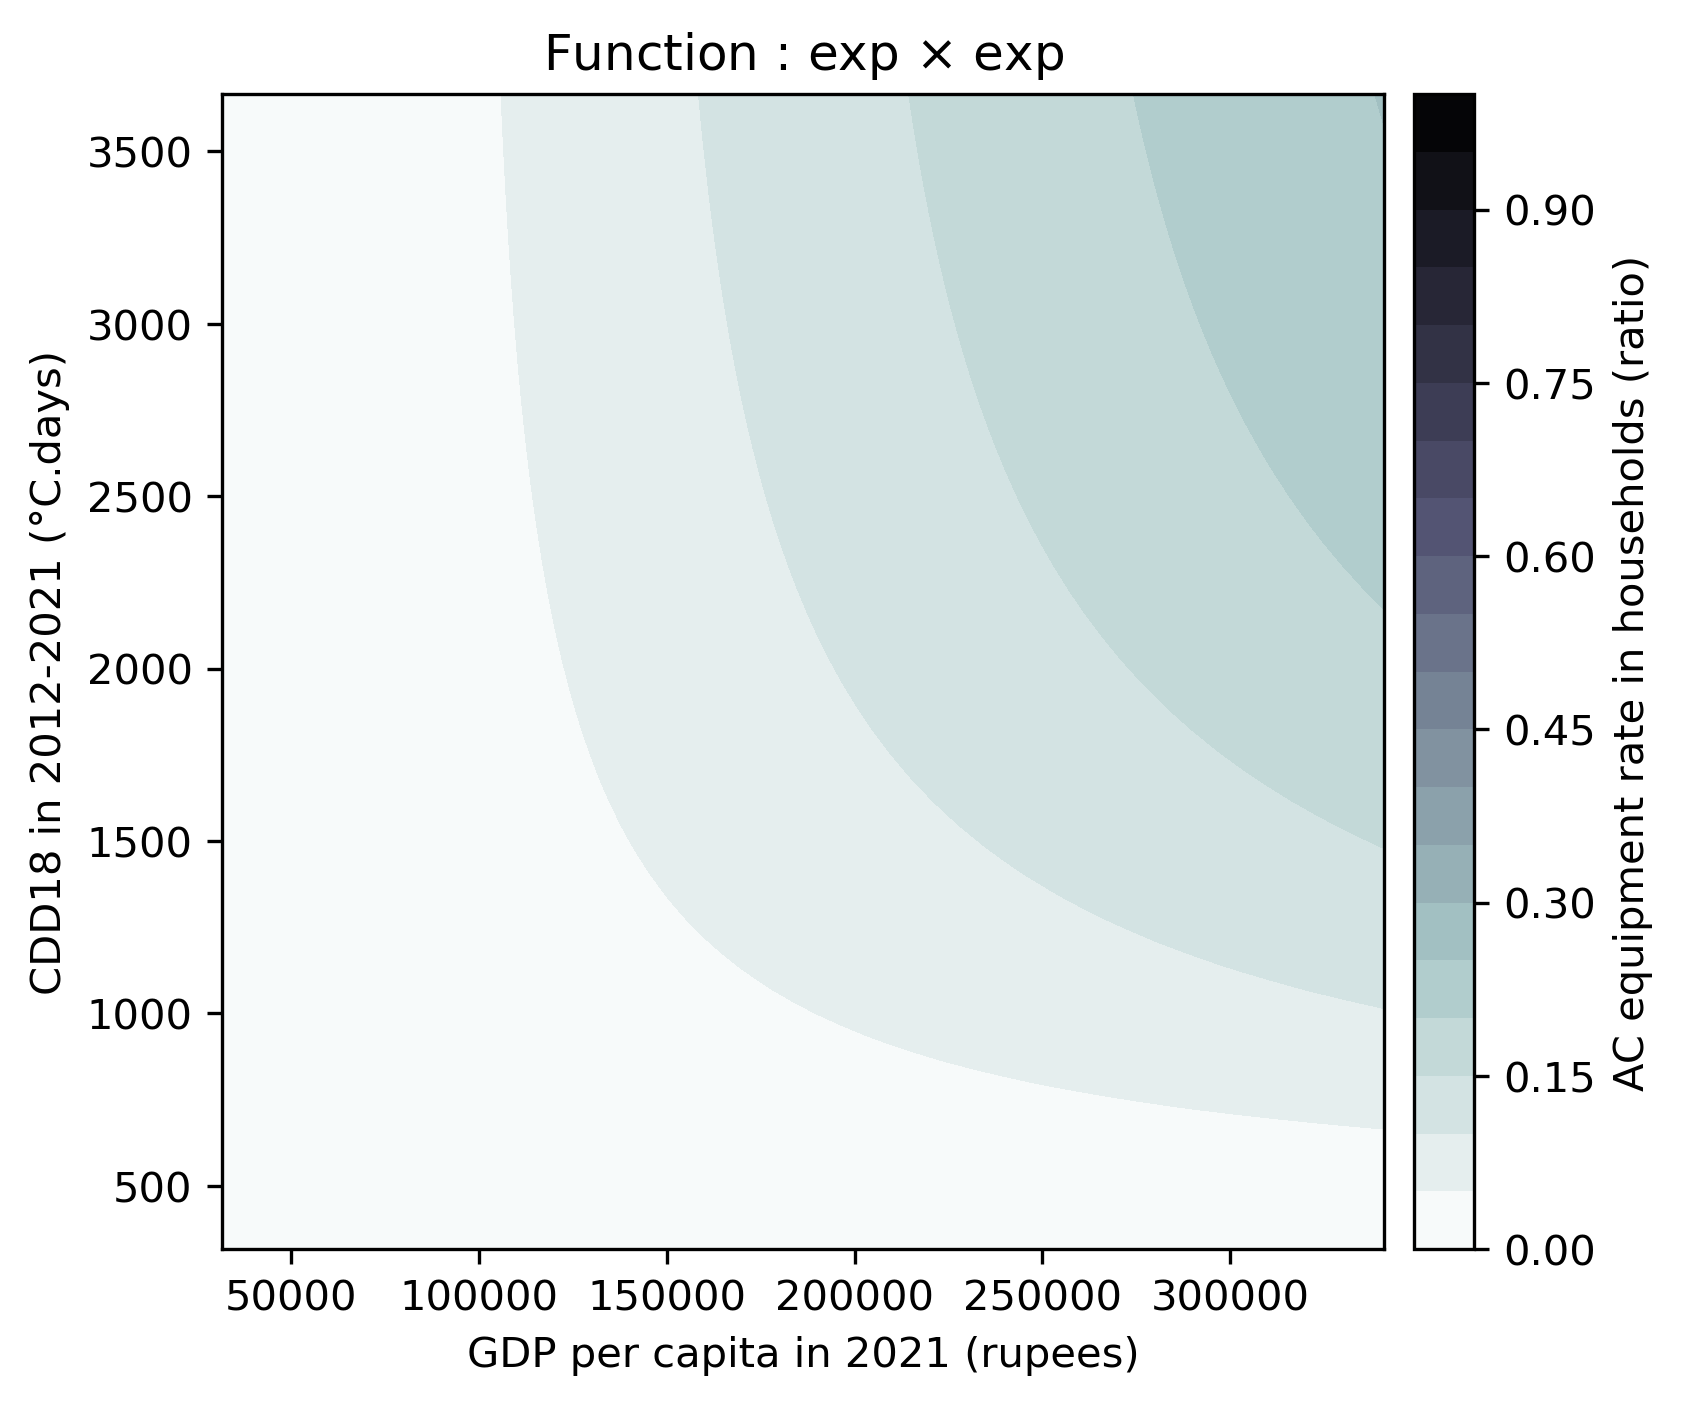
\includegraphics[width=0.38\columnwidth]{figures/cdd18_exp_exp_2dplot.png}

   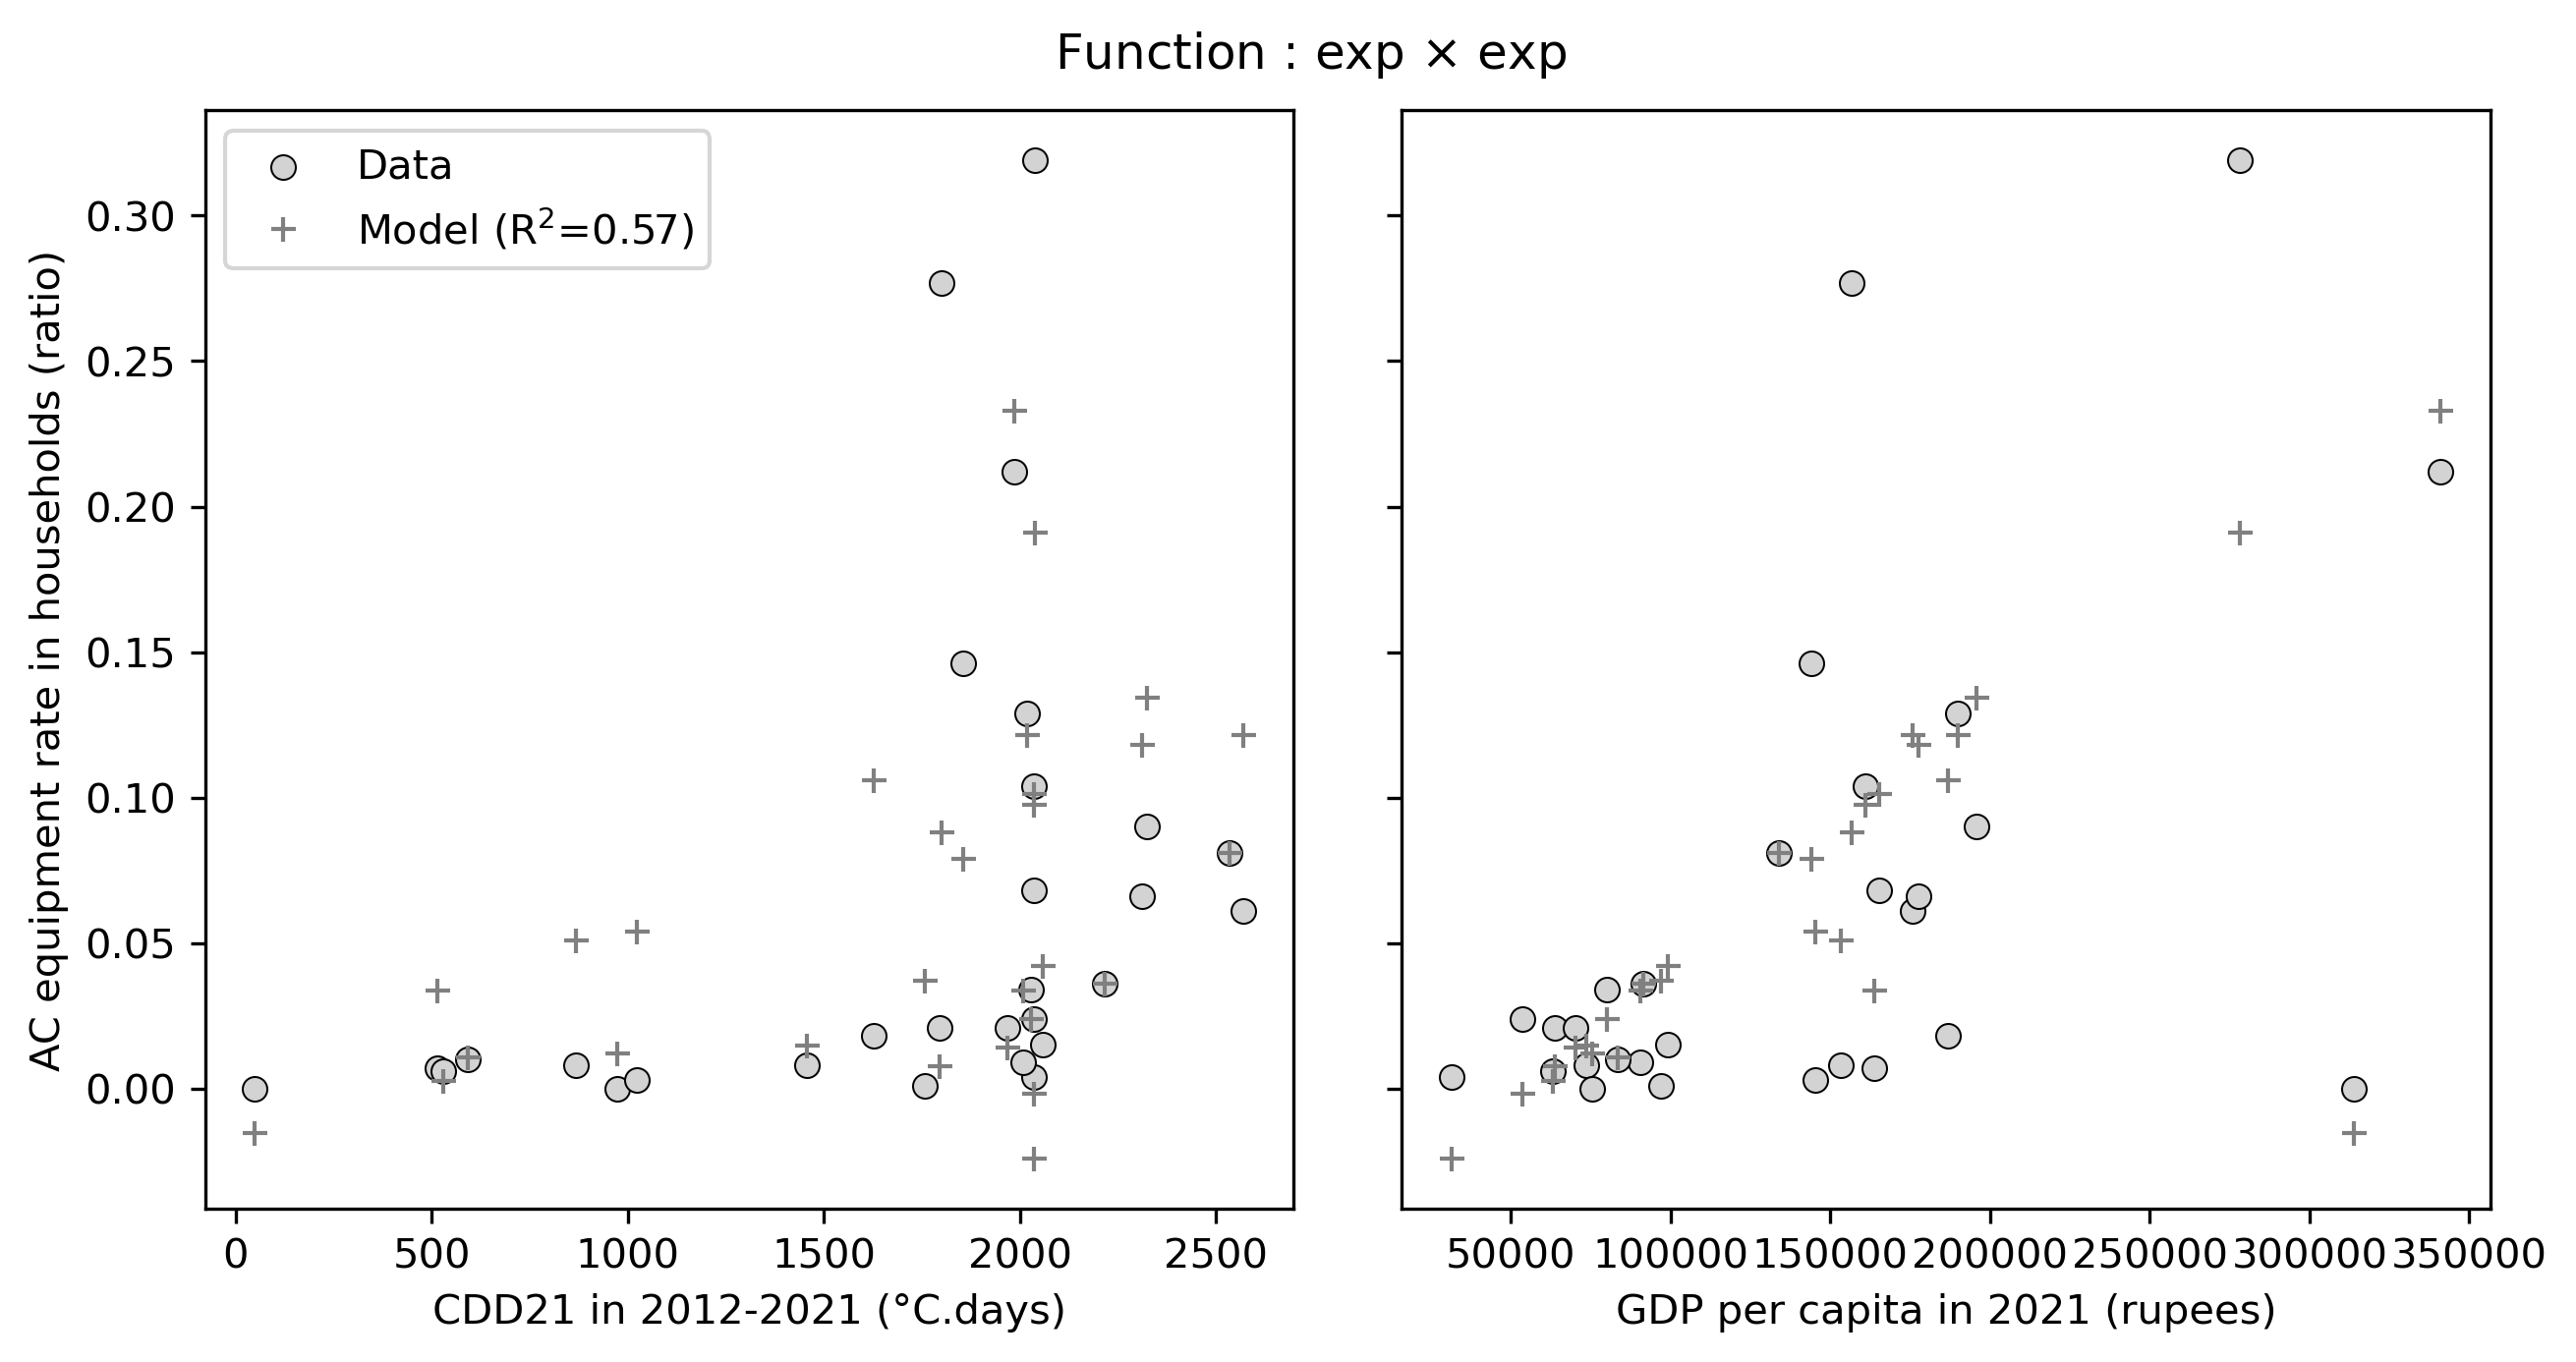
\includegraphics[width=0.6\columnwidth]{figures/cdd21_exp_exp_scatter.png}
   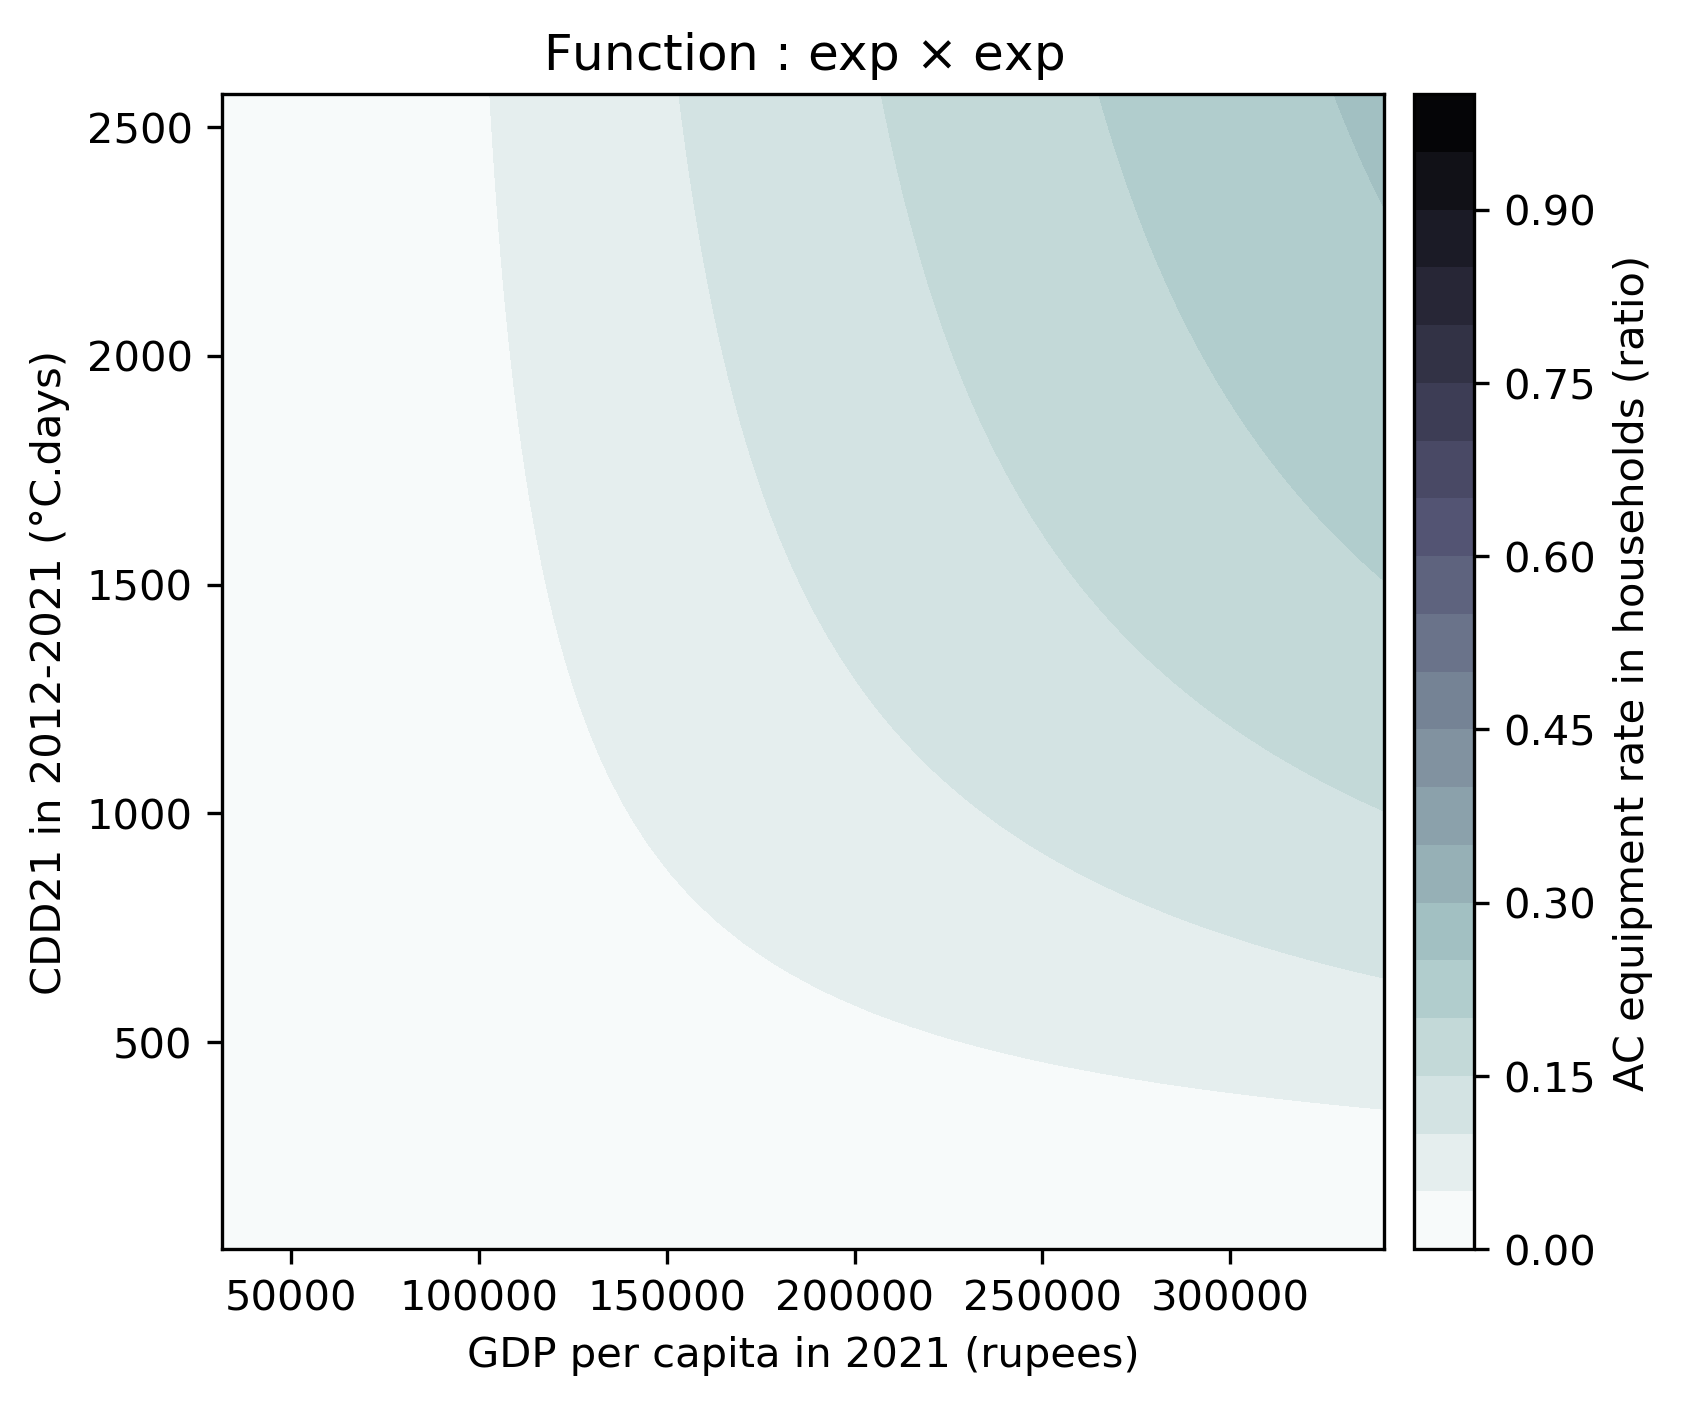
\includegraphics[width=0.38\columnwidth]{figures/cdd21_exp_exp_2dplot.png}

   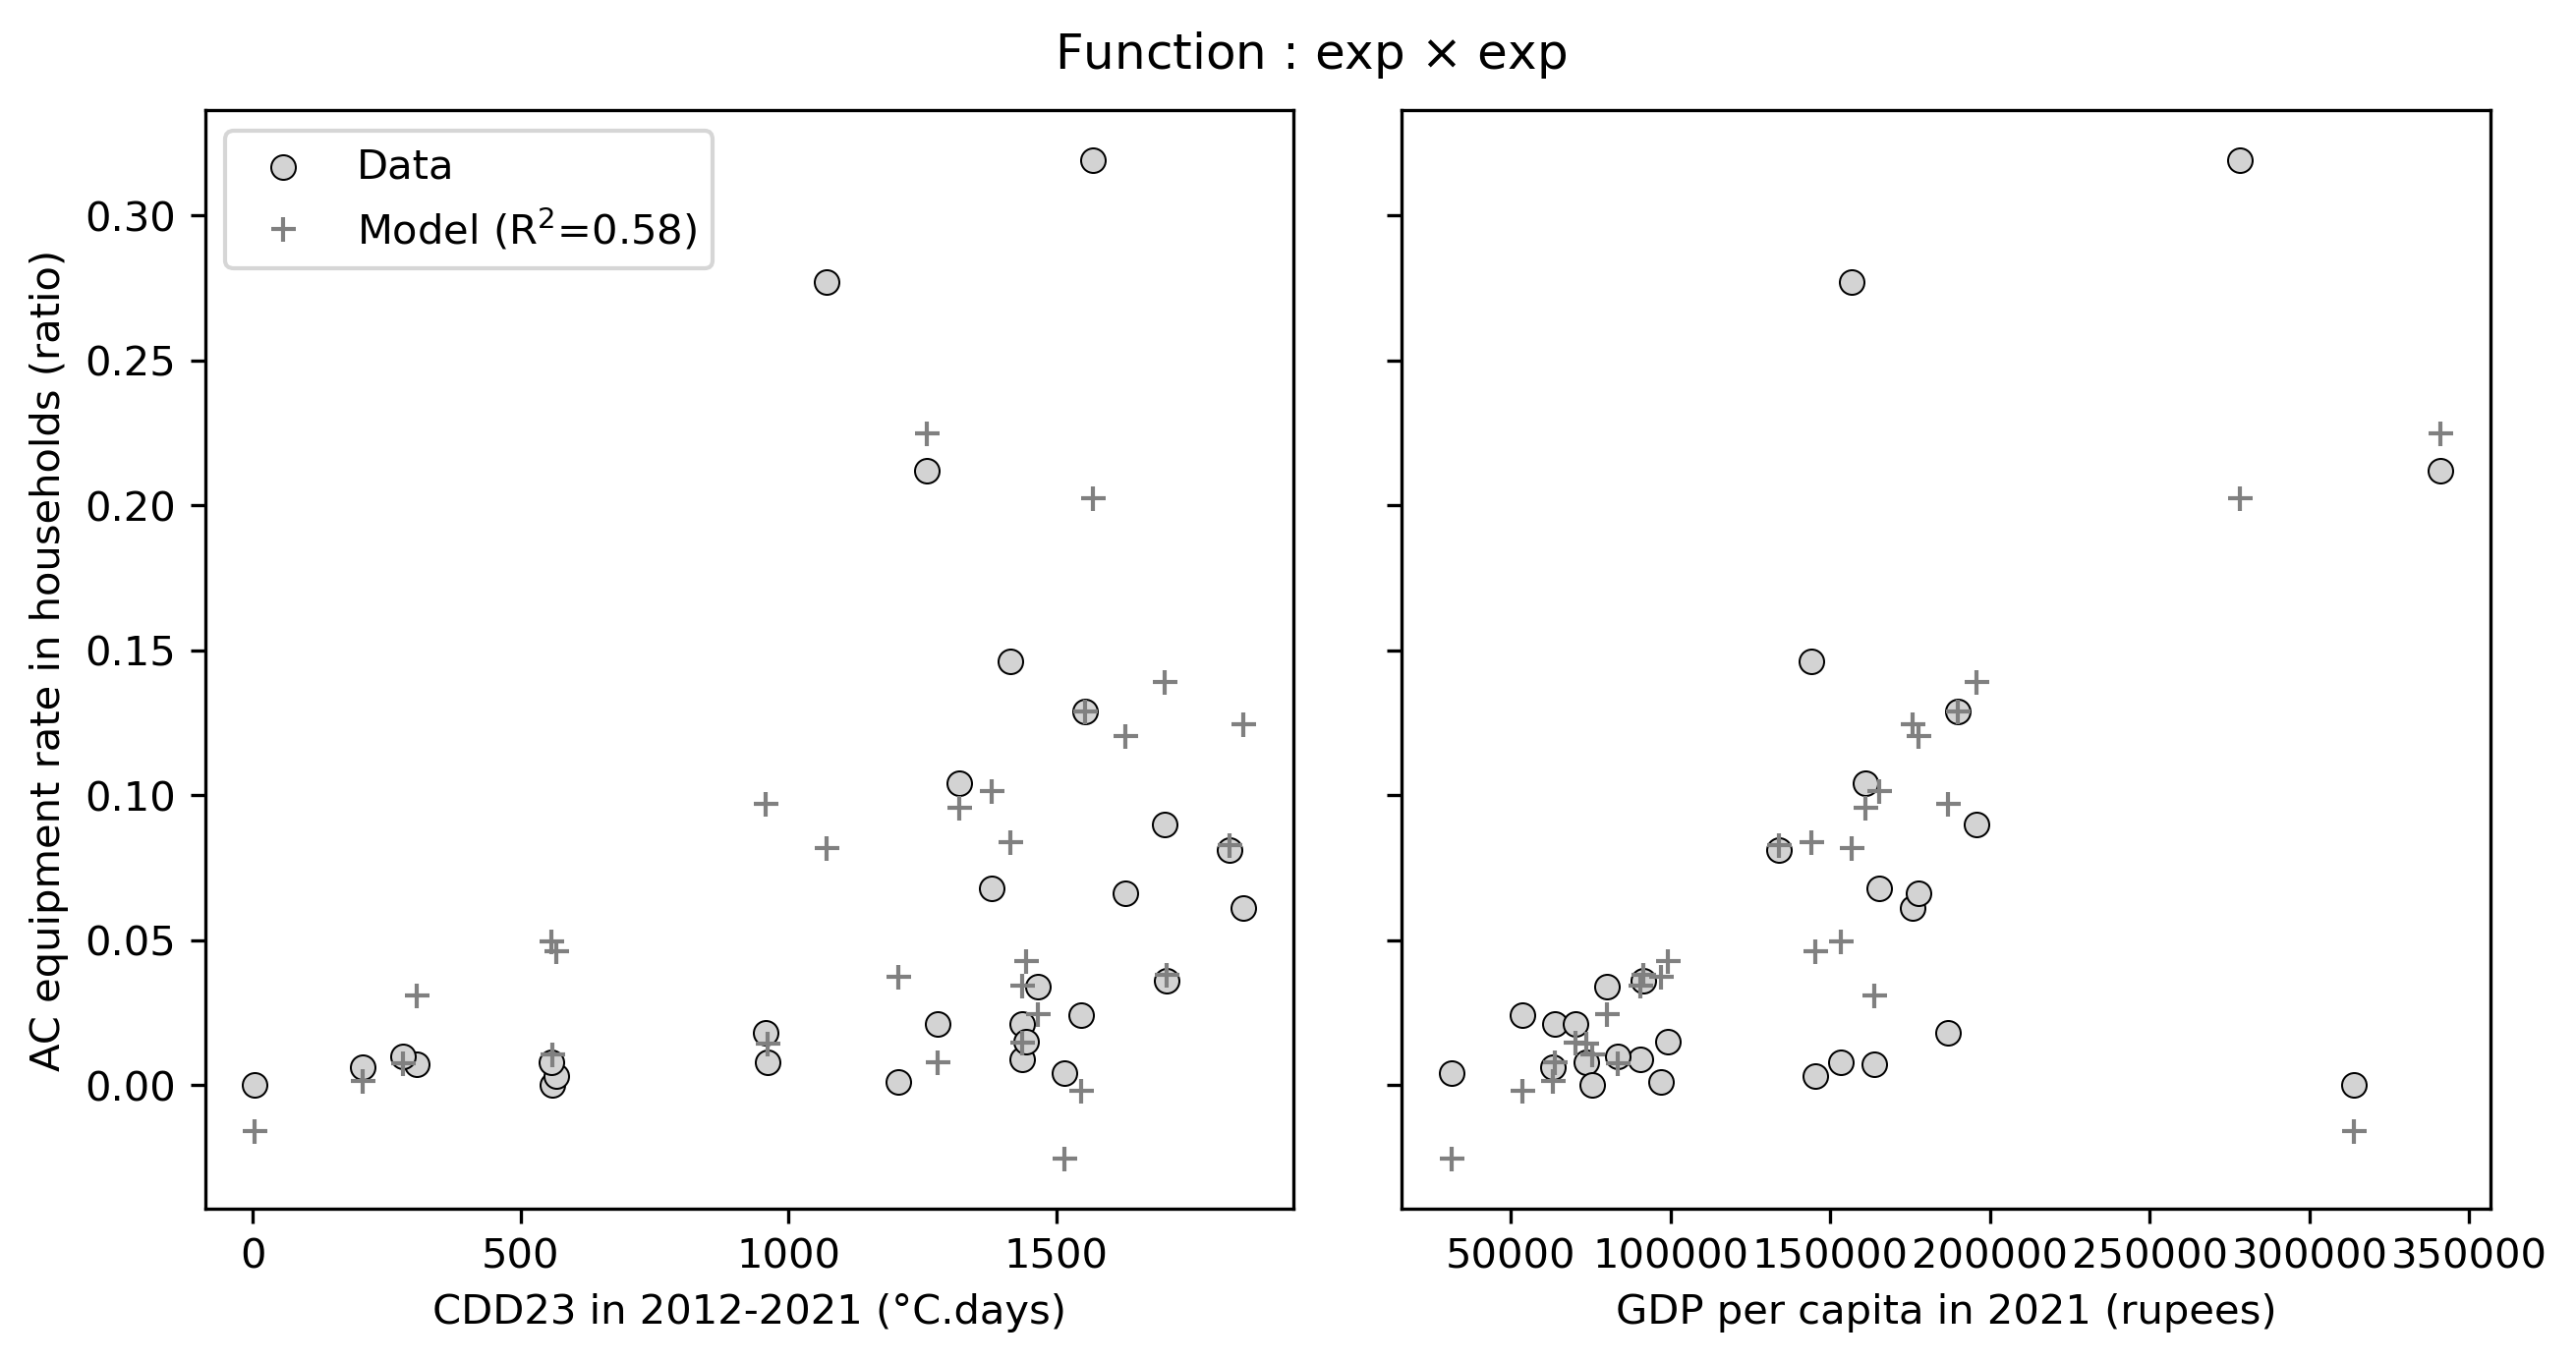
\includegraphics[width=0.6\columnwidth]{figures/cdd23_exp_exp_scatter.png}
   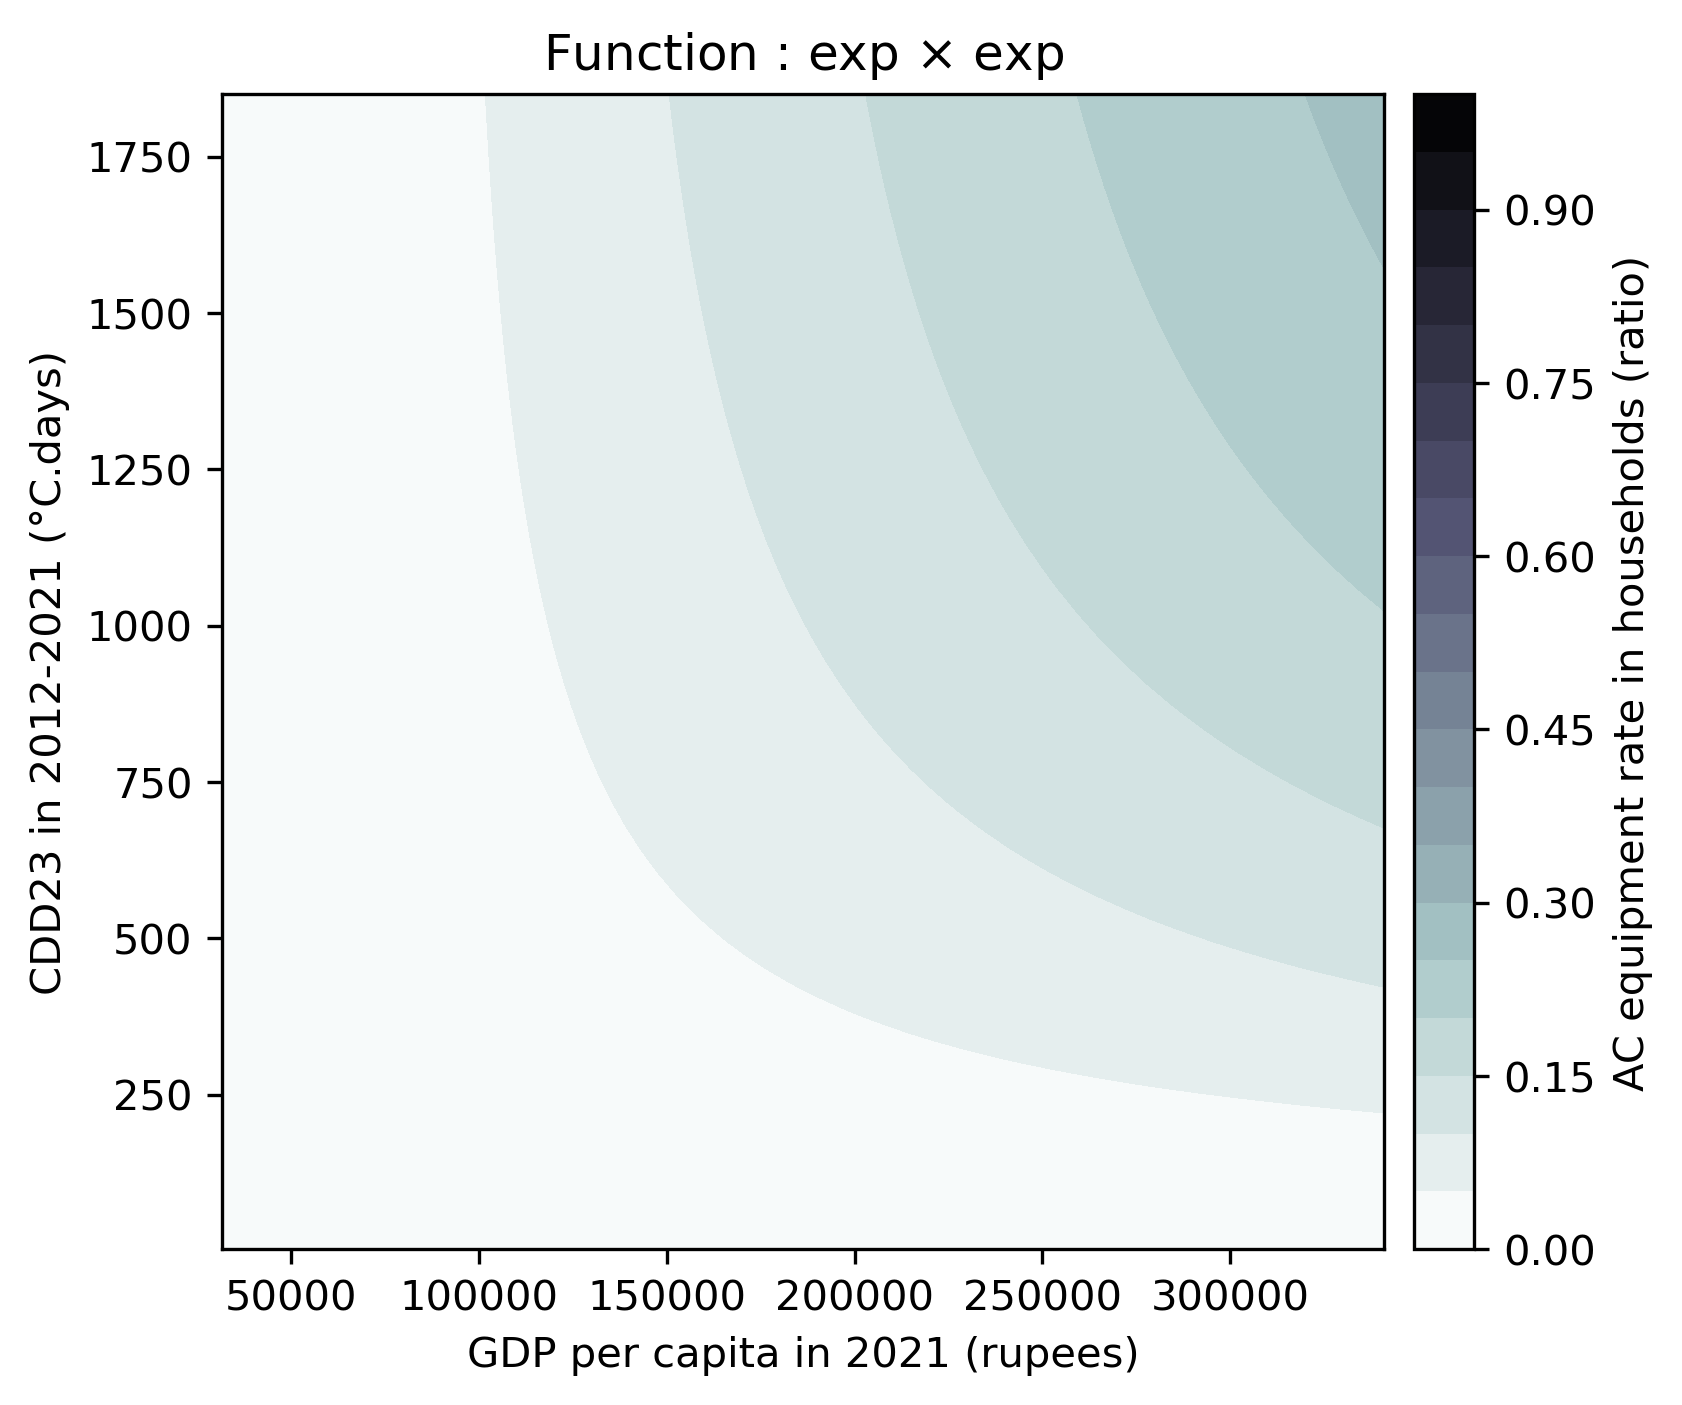
\includegraphics[width=0.38\columnwidth]{figures/cdd23_exp_exp_2dplot.png}

   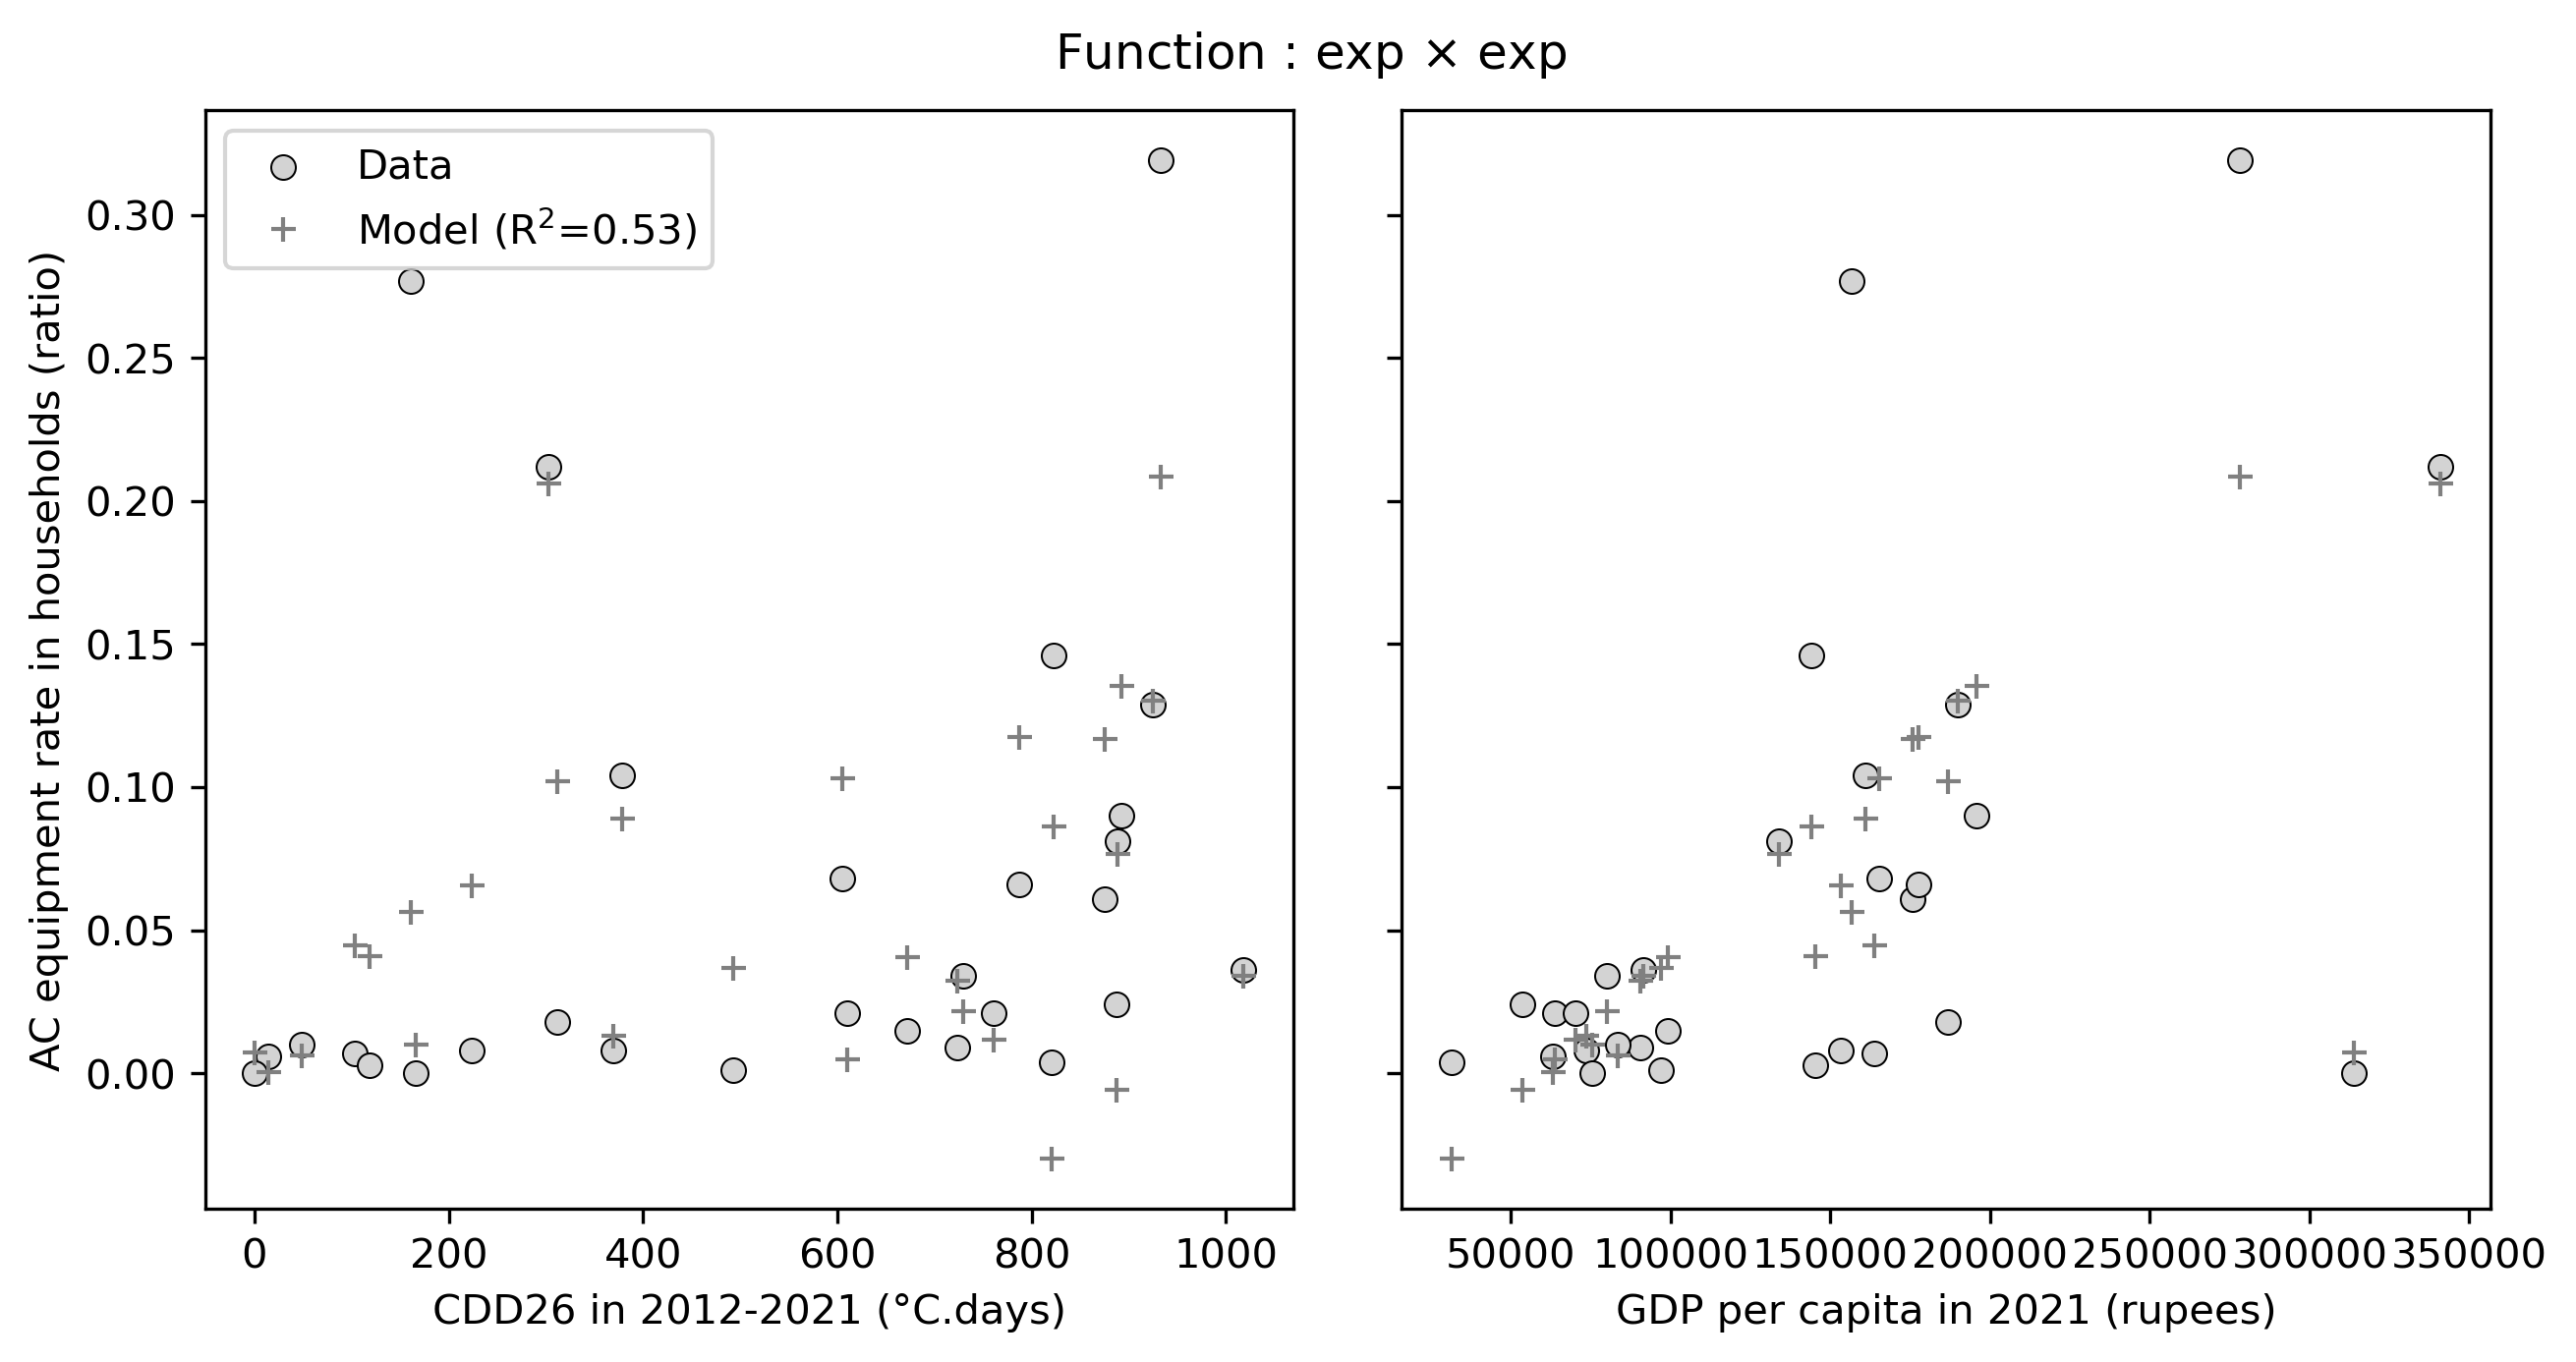
\includegraphics[width=0.6\columnwidth]{figures/cdd26_exp_exp_scatter.png}
   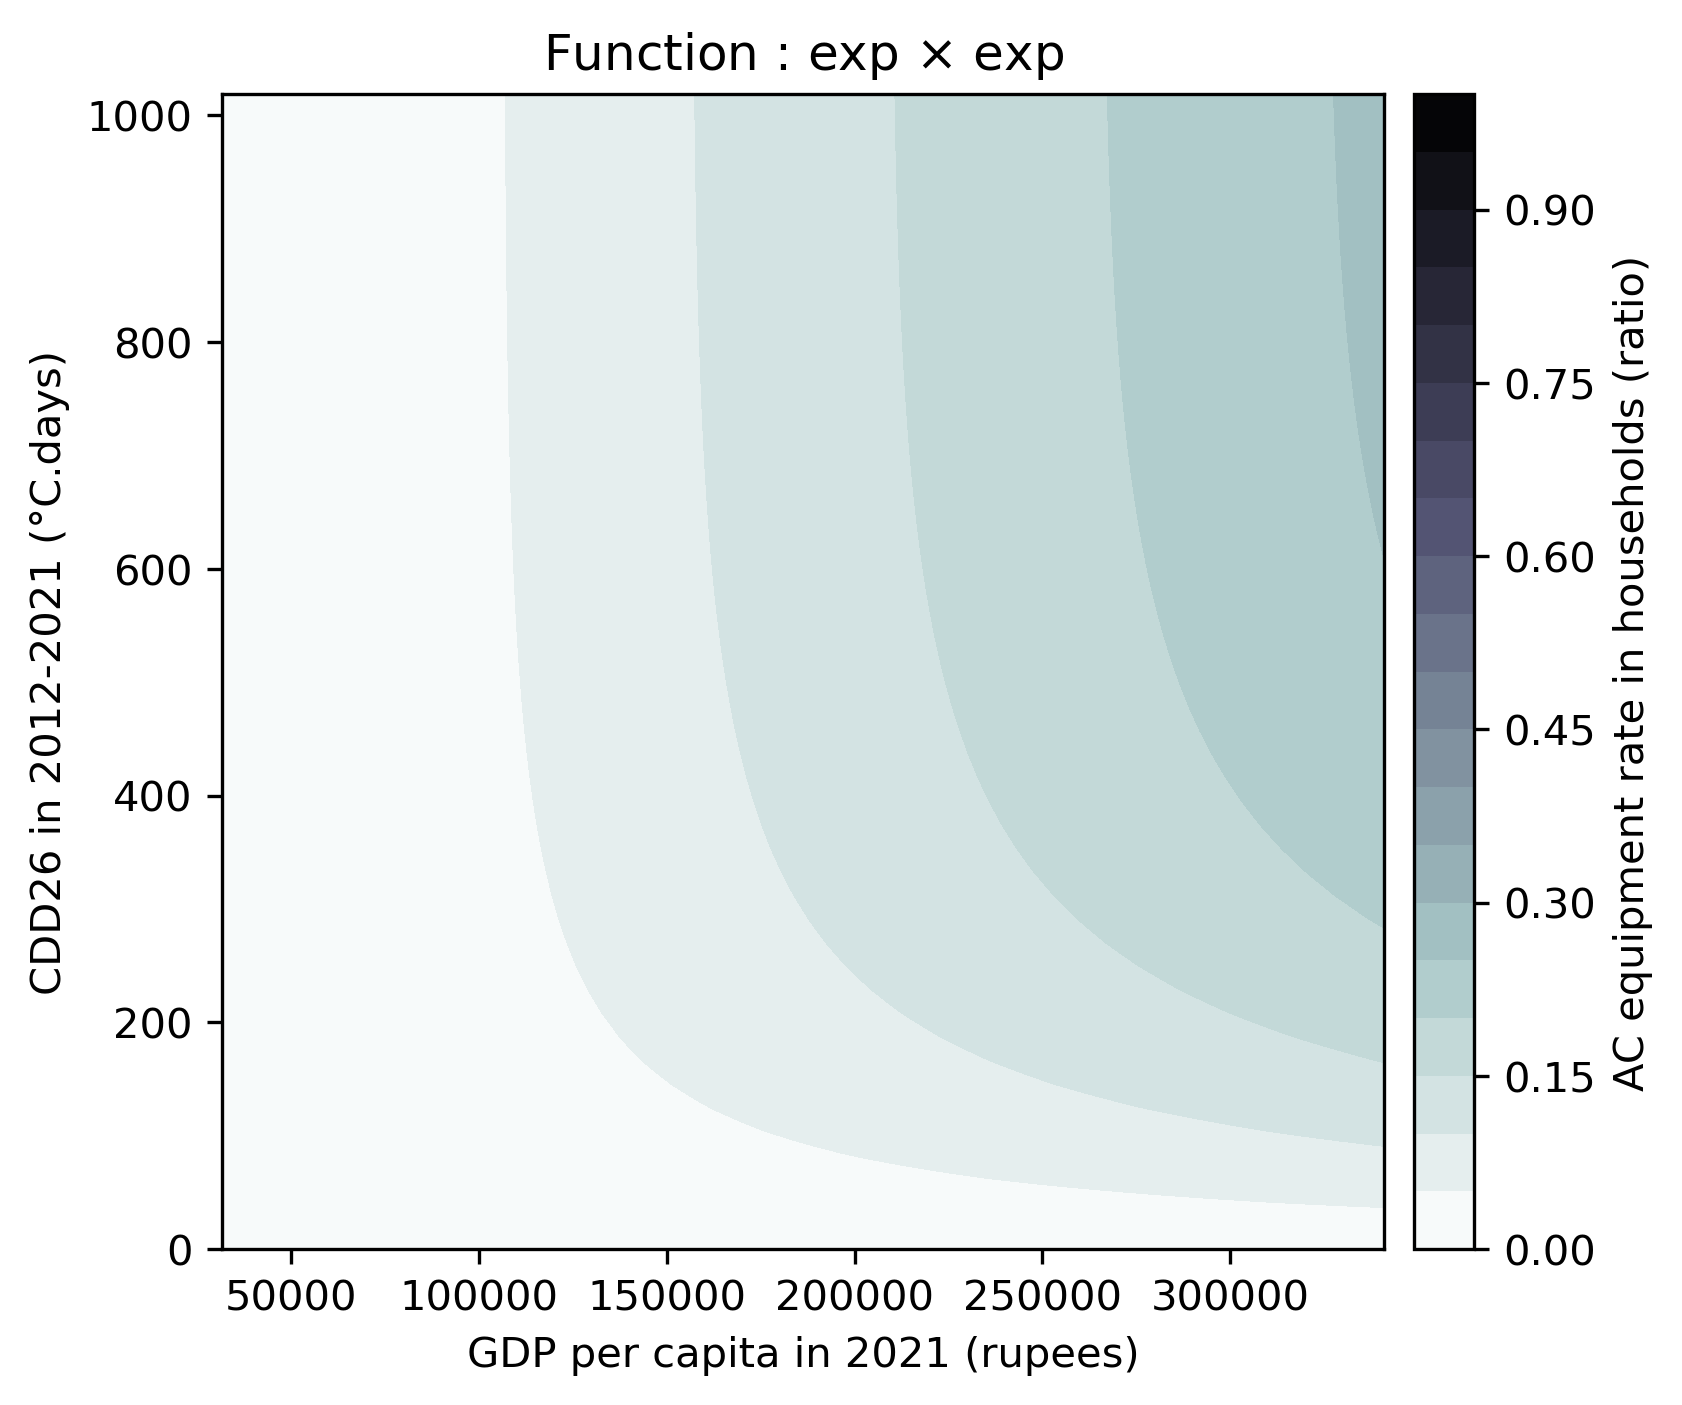
\includegraphics[width=0.38\columnwidth]{figures/cdd26_exp_exp_2dplot.png}
   \caption{\label{fig:ee} Résultats de modélisation. De haut en bas, CDD à seuils de 18, 21, 23 et \SI{26}{\celsius}.}
\end{figure}

\clearpage 
\subsection{Modèle $\mathrm{S-E}$}

\begin{figure}[ht]
   \centering
   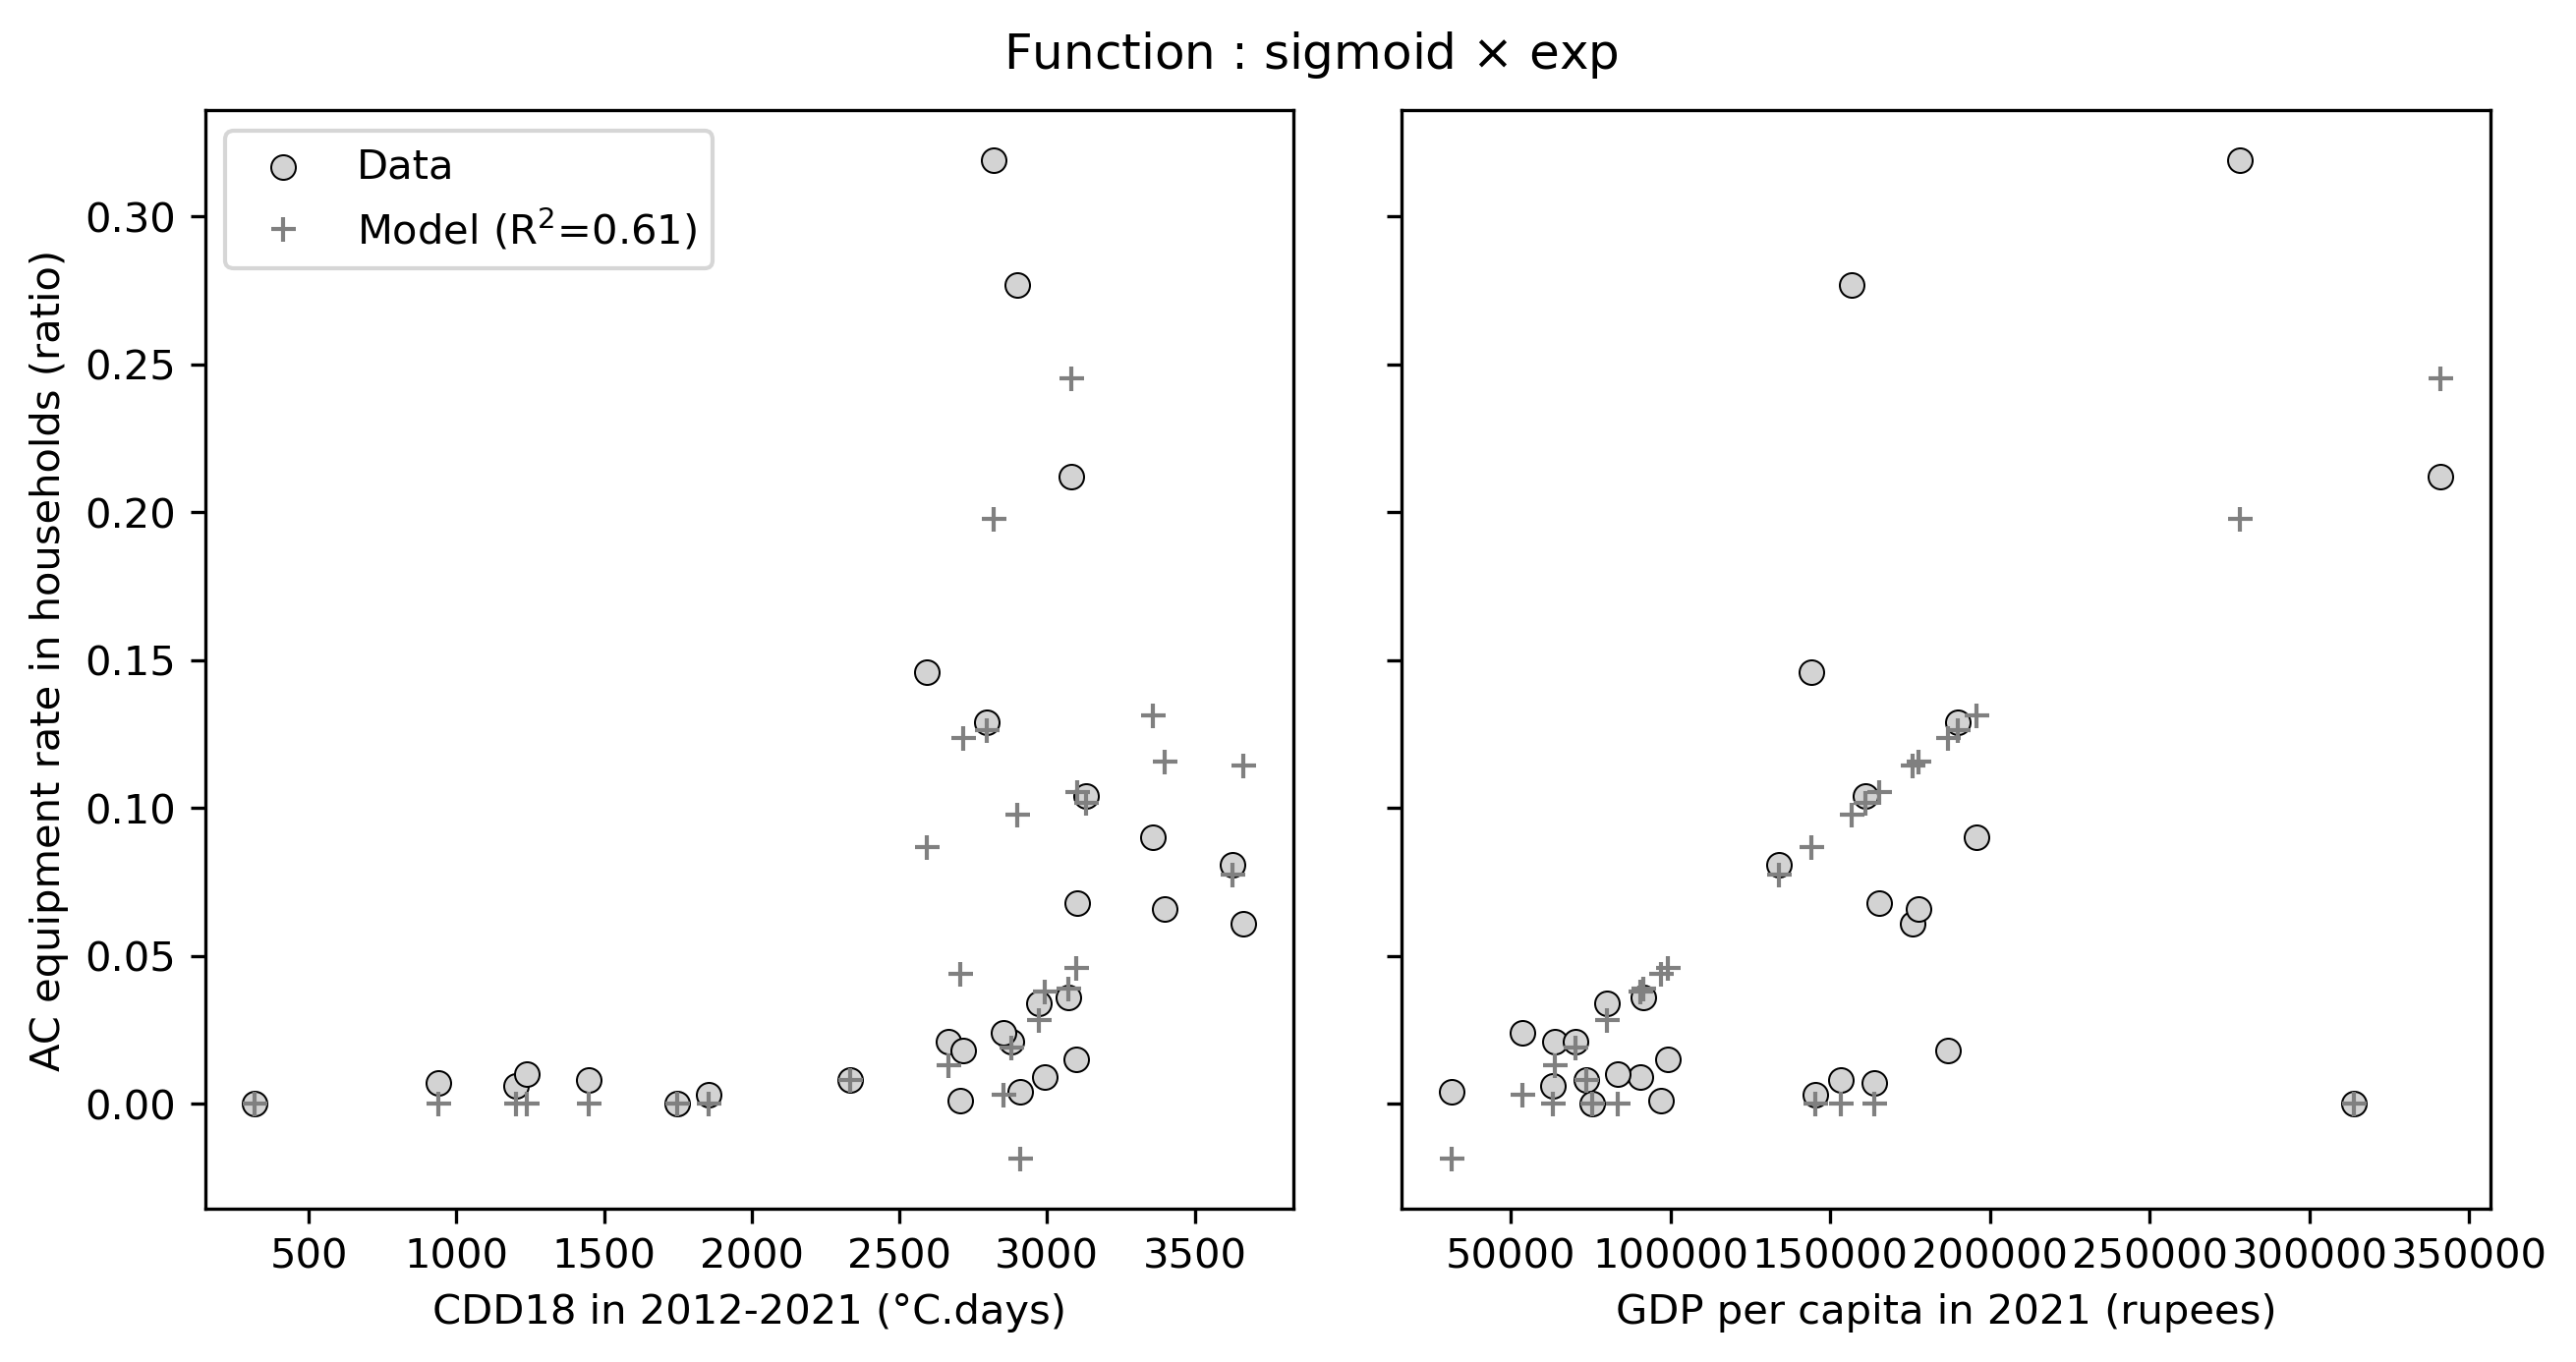
\includegraphics[width=0.6\columnwidth]{figures/cdd18_sigmoid_exp_scatter.png}
   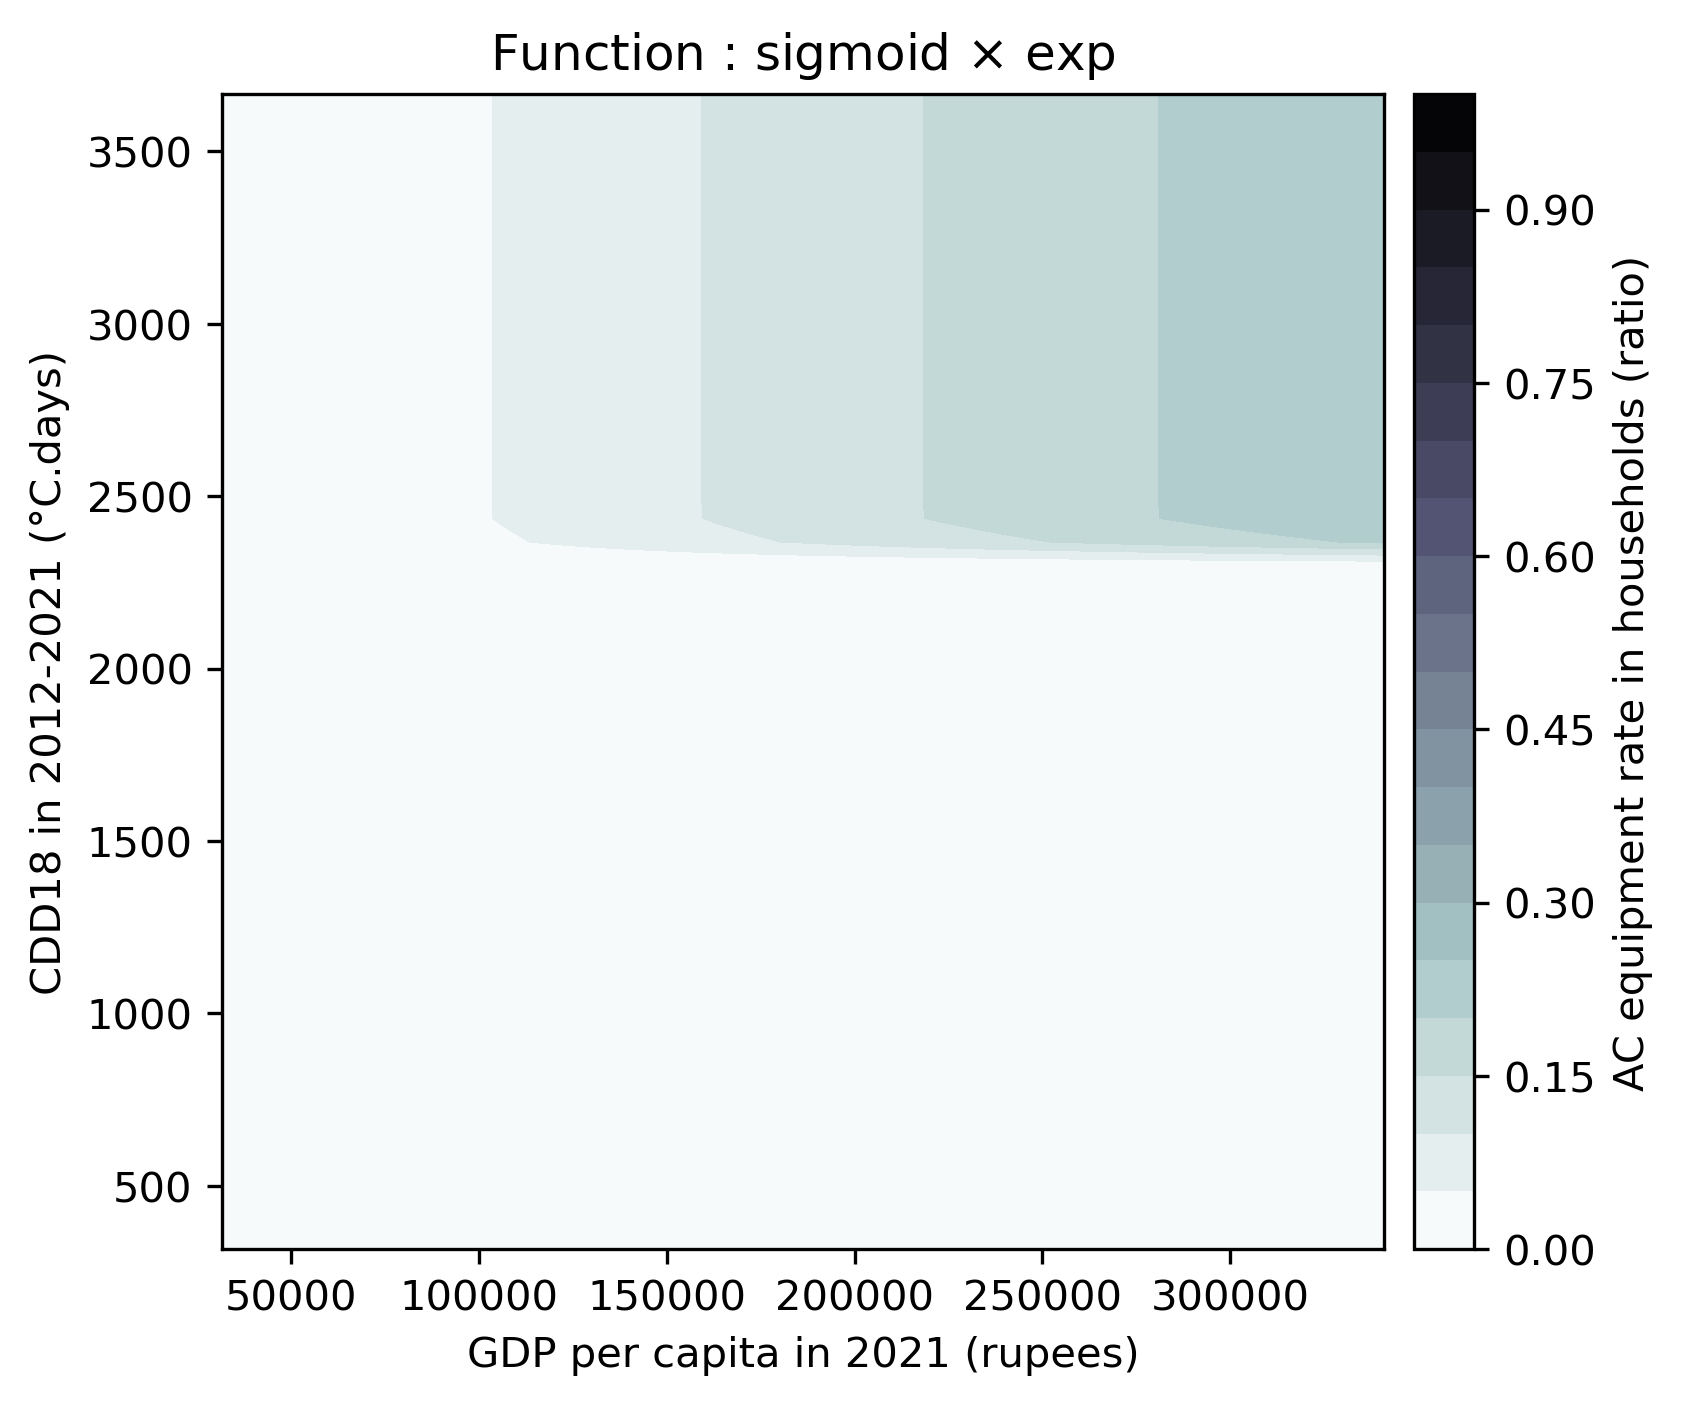
\includegraphics[width=0.38\columnwidth]{figures/cdd18_sigmoid_exp_2dplot.png}

   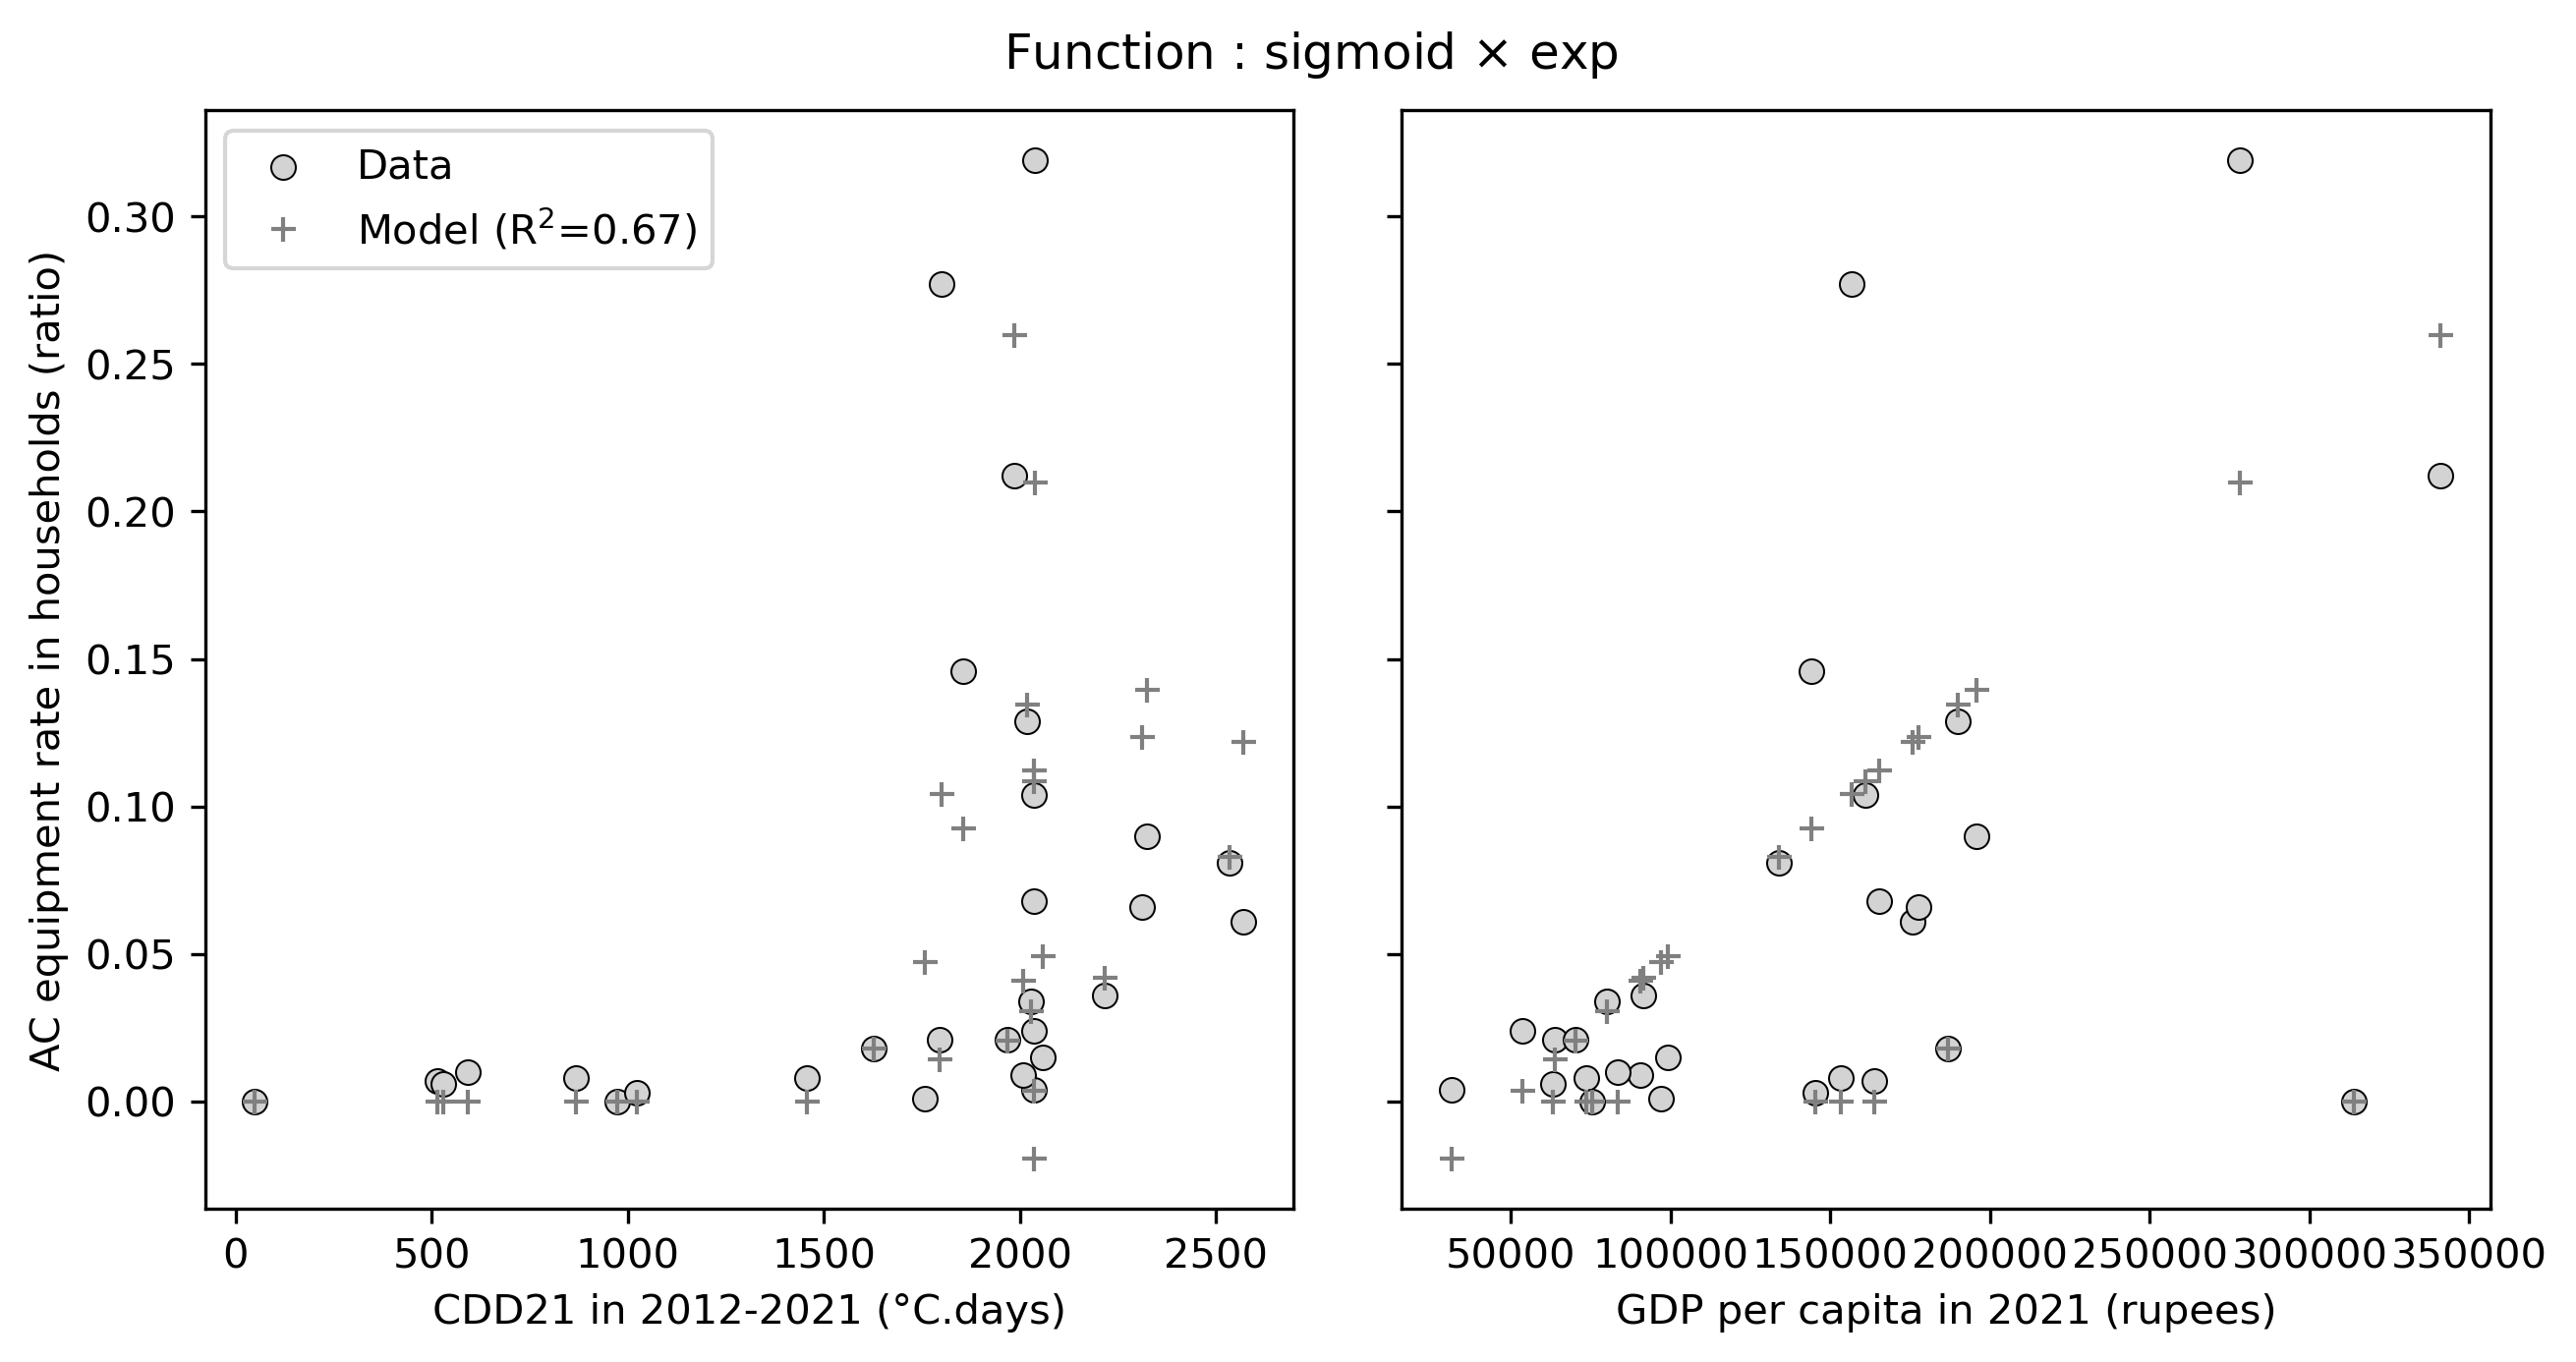
\includegraphics[width=0.6\columnwidth]{figures/cdd21_sigmoid_exp_scatter.png}
   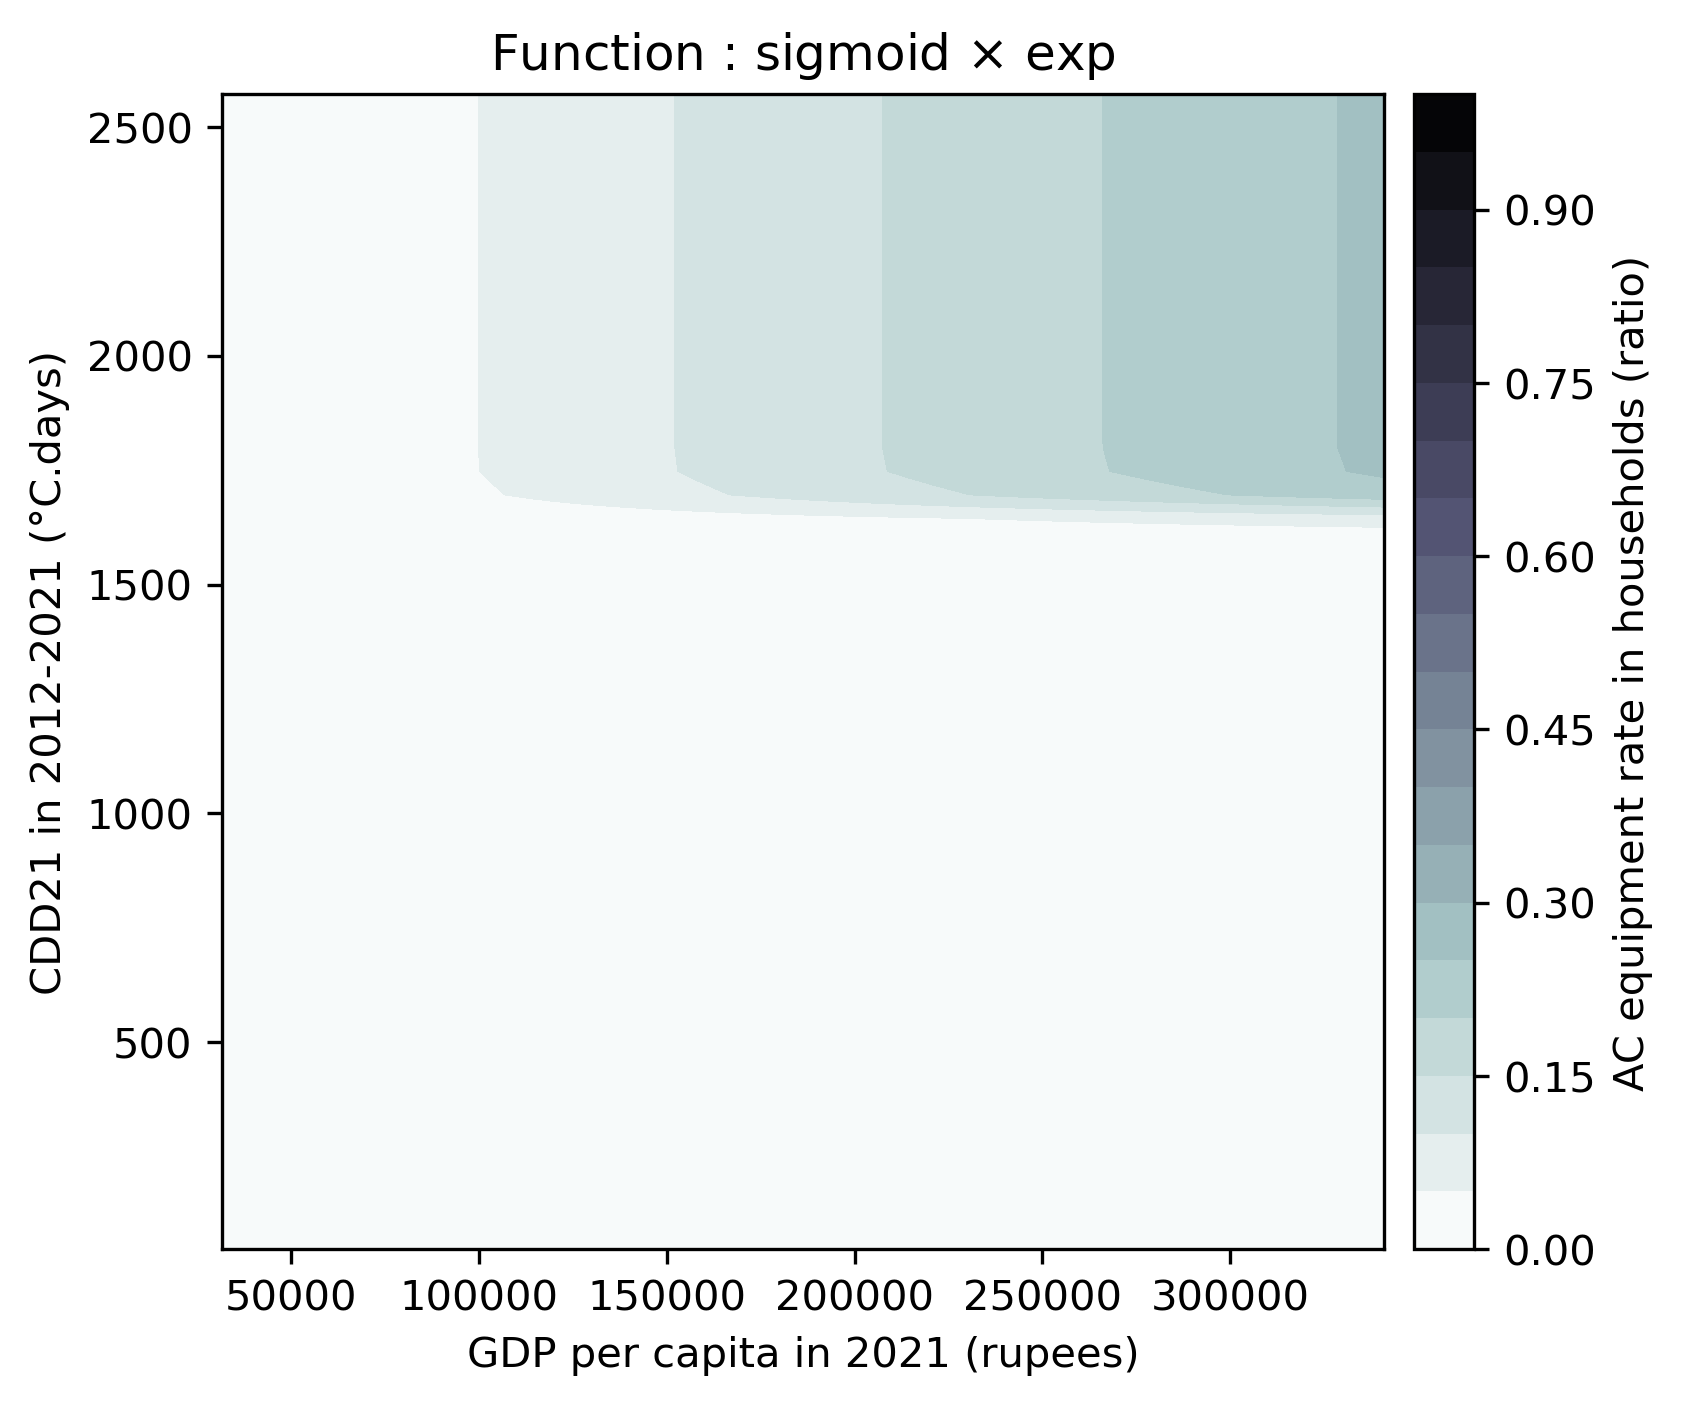
\includegraphics[width=0.38\columnwidth]{figures/cdd21_sigmoid_exp_2dplot.png}

   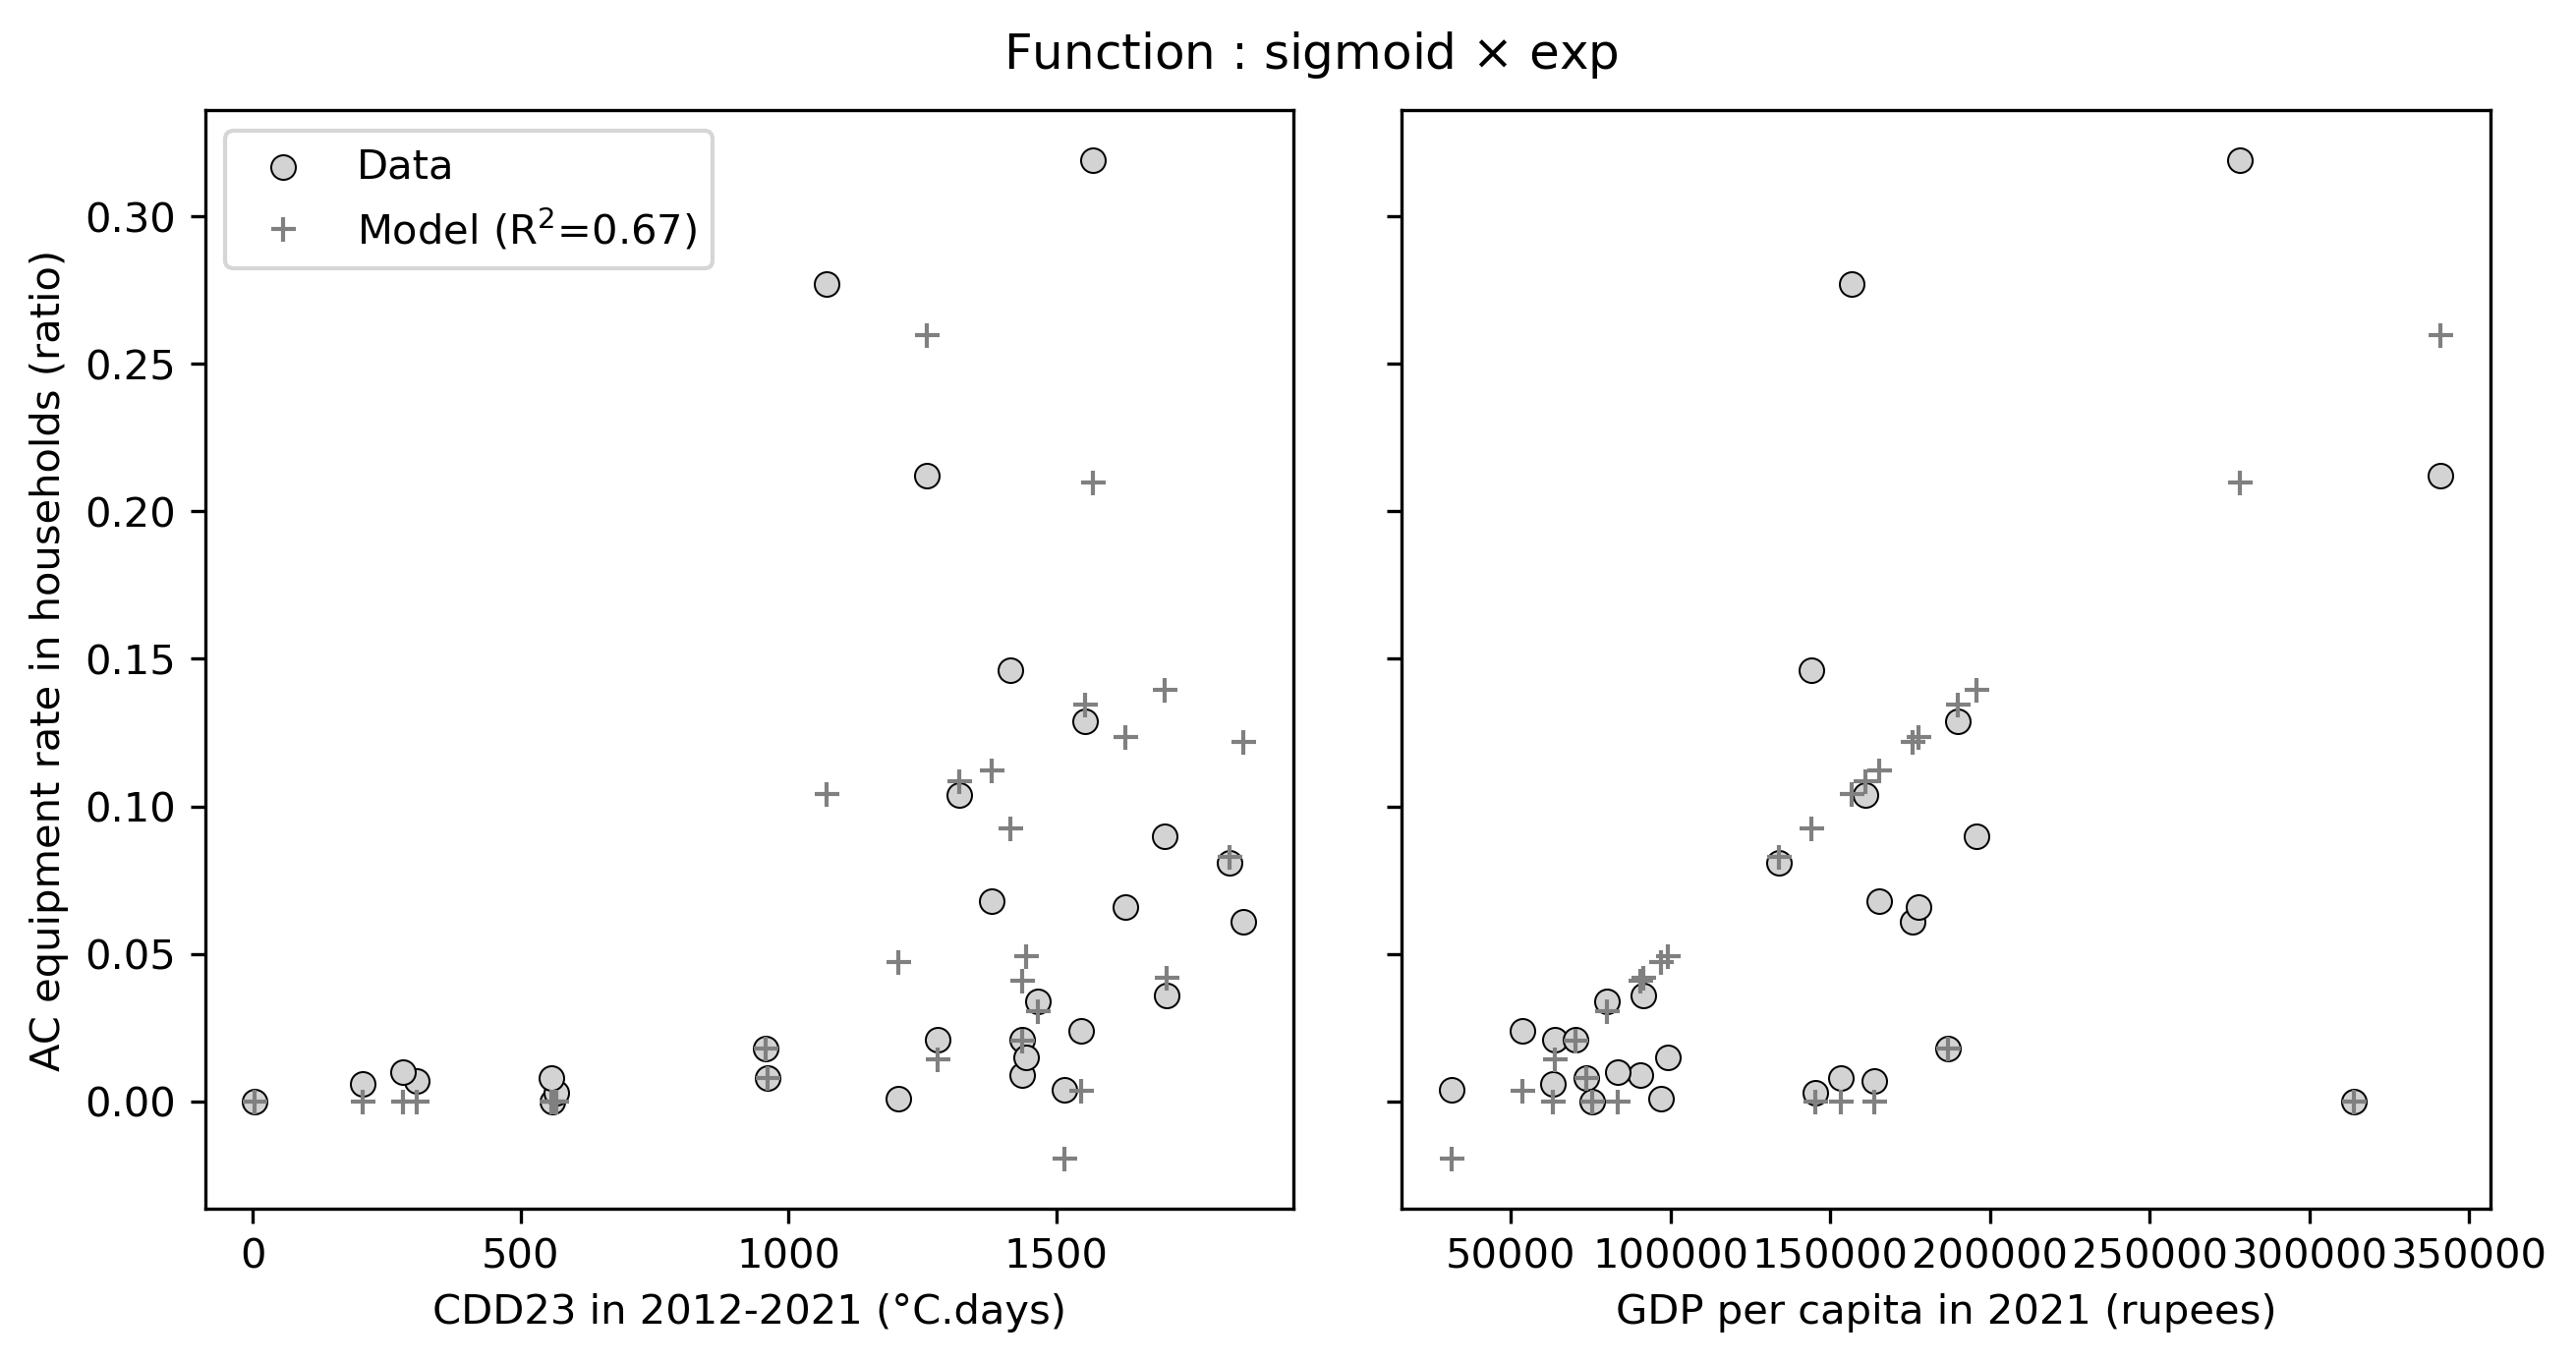
\includegraphics[width=0.6\columnwidth]{figures/cdd23_sigmoid_exp_scatter.png}
   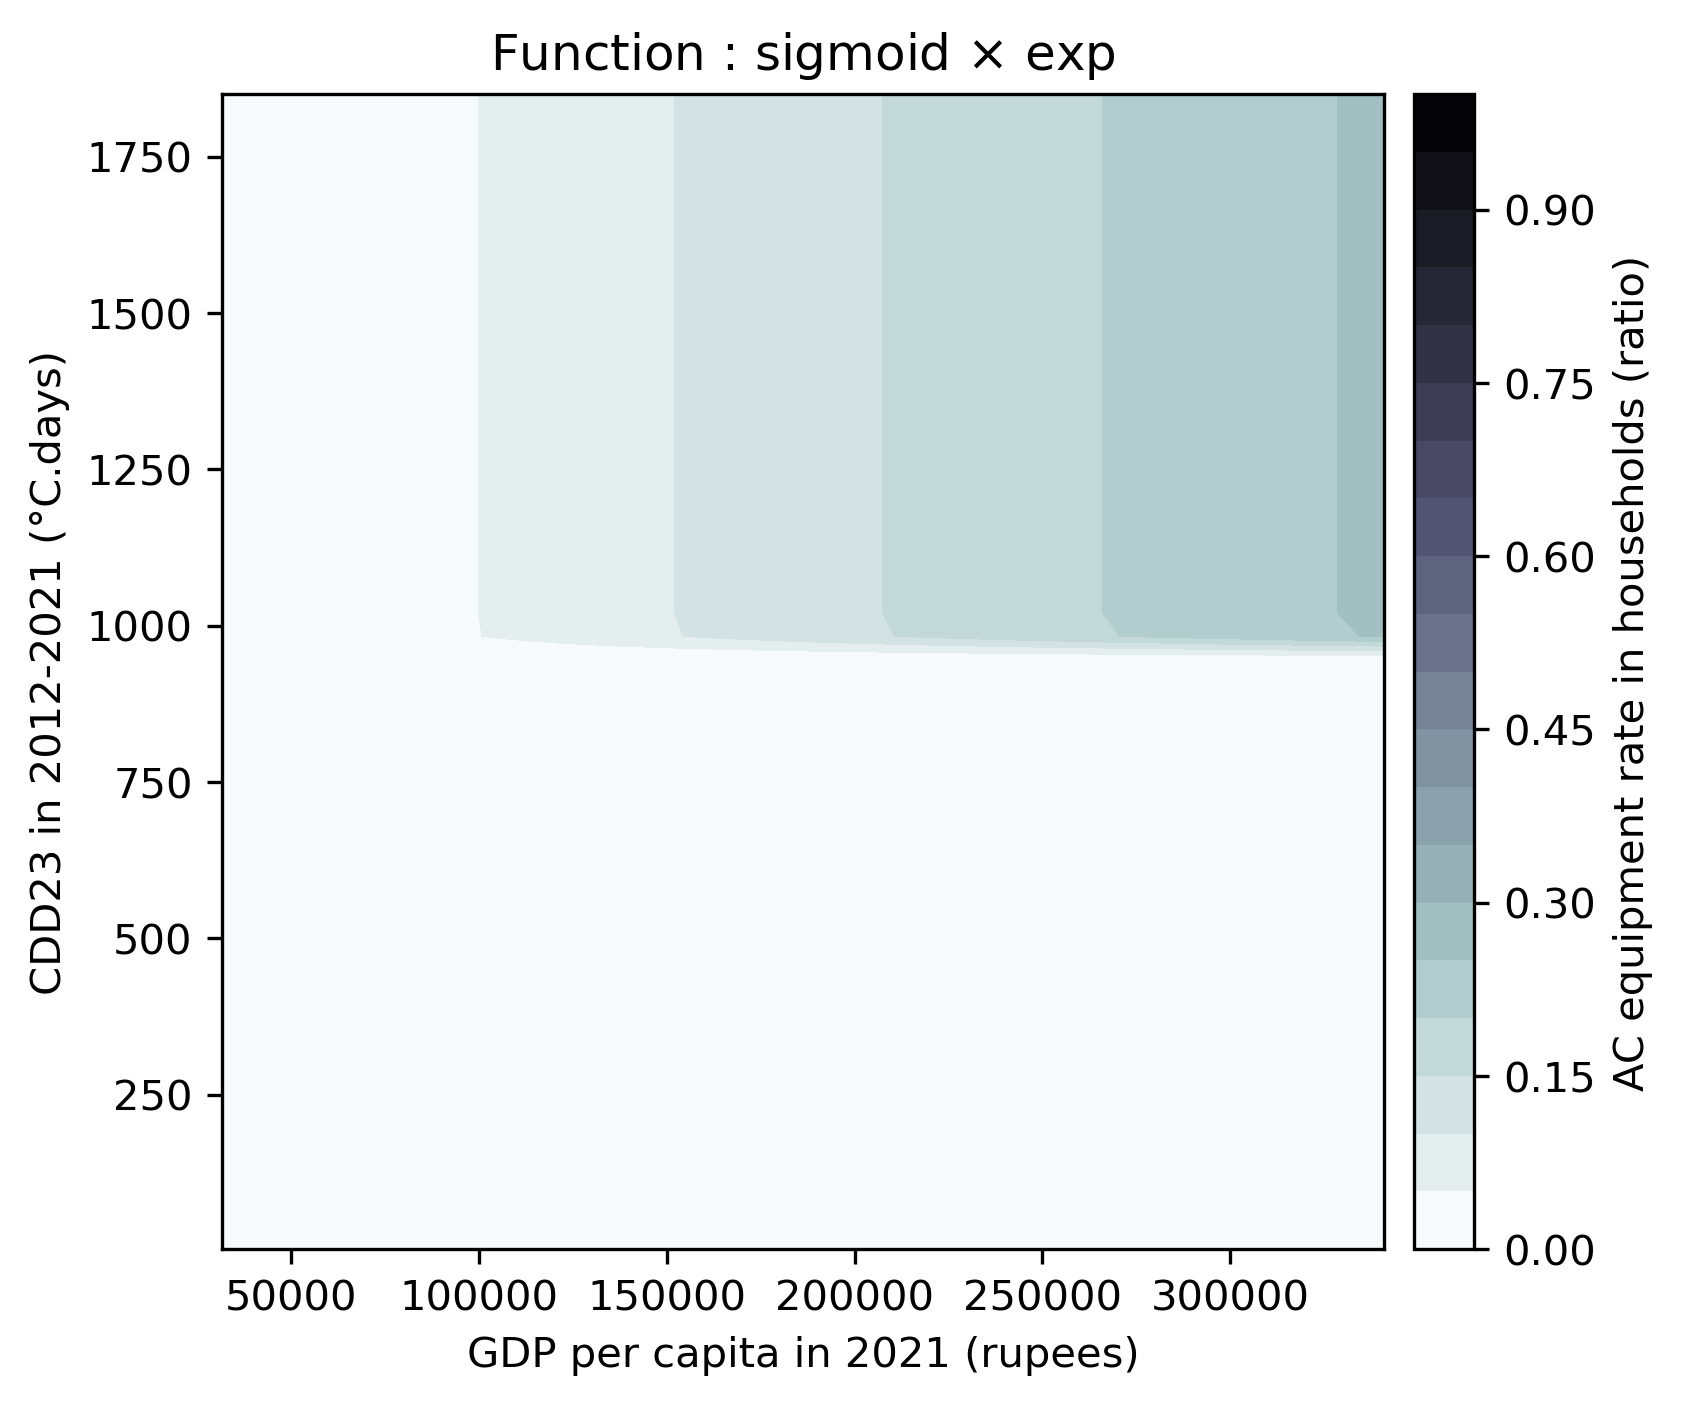
\includegraphics[width=0.38\columnwidth]{figures/cdd23_sigmoid_exp_2dplot.png}

   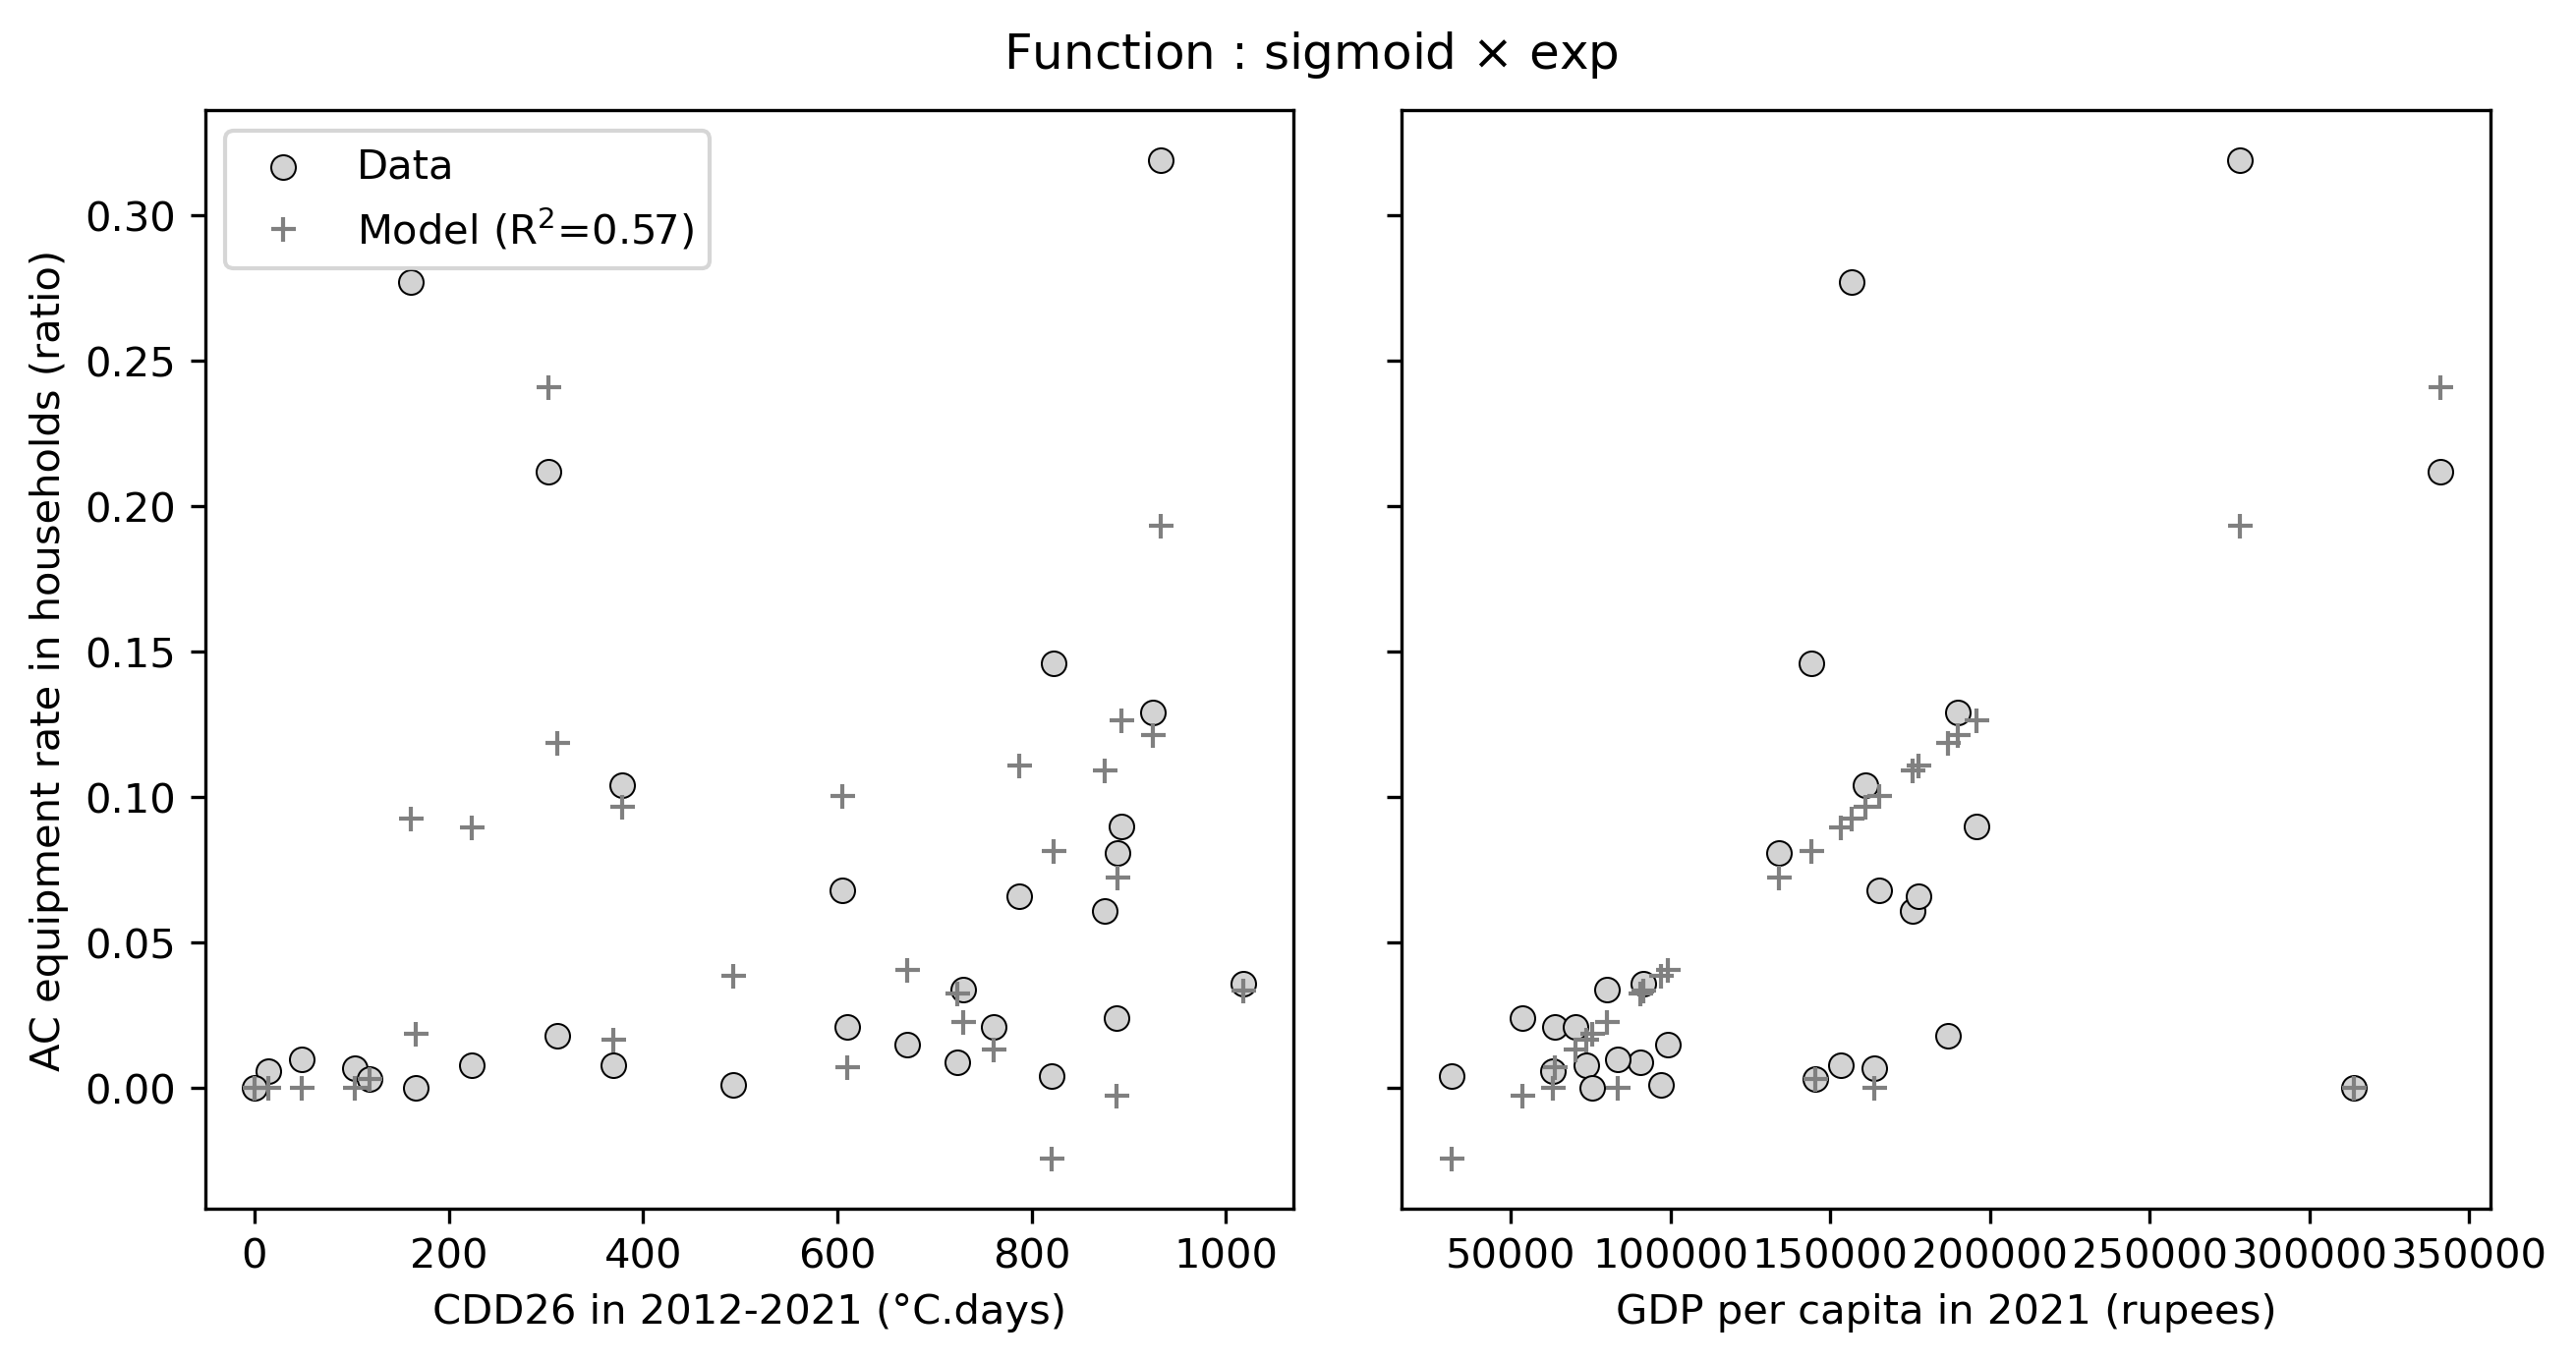
\includegraphics[width=0.6\columnwidth]{figures/cdd26_sigmoid_exp_scatter.png}
   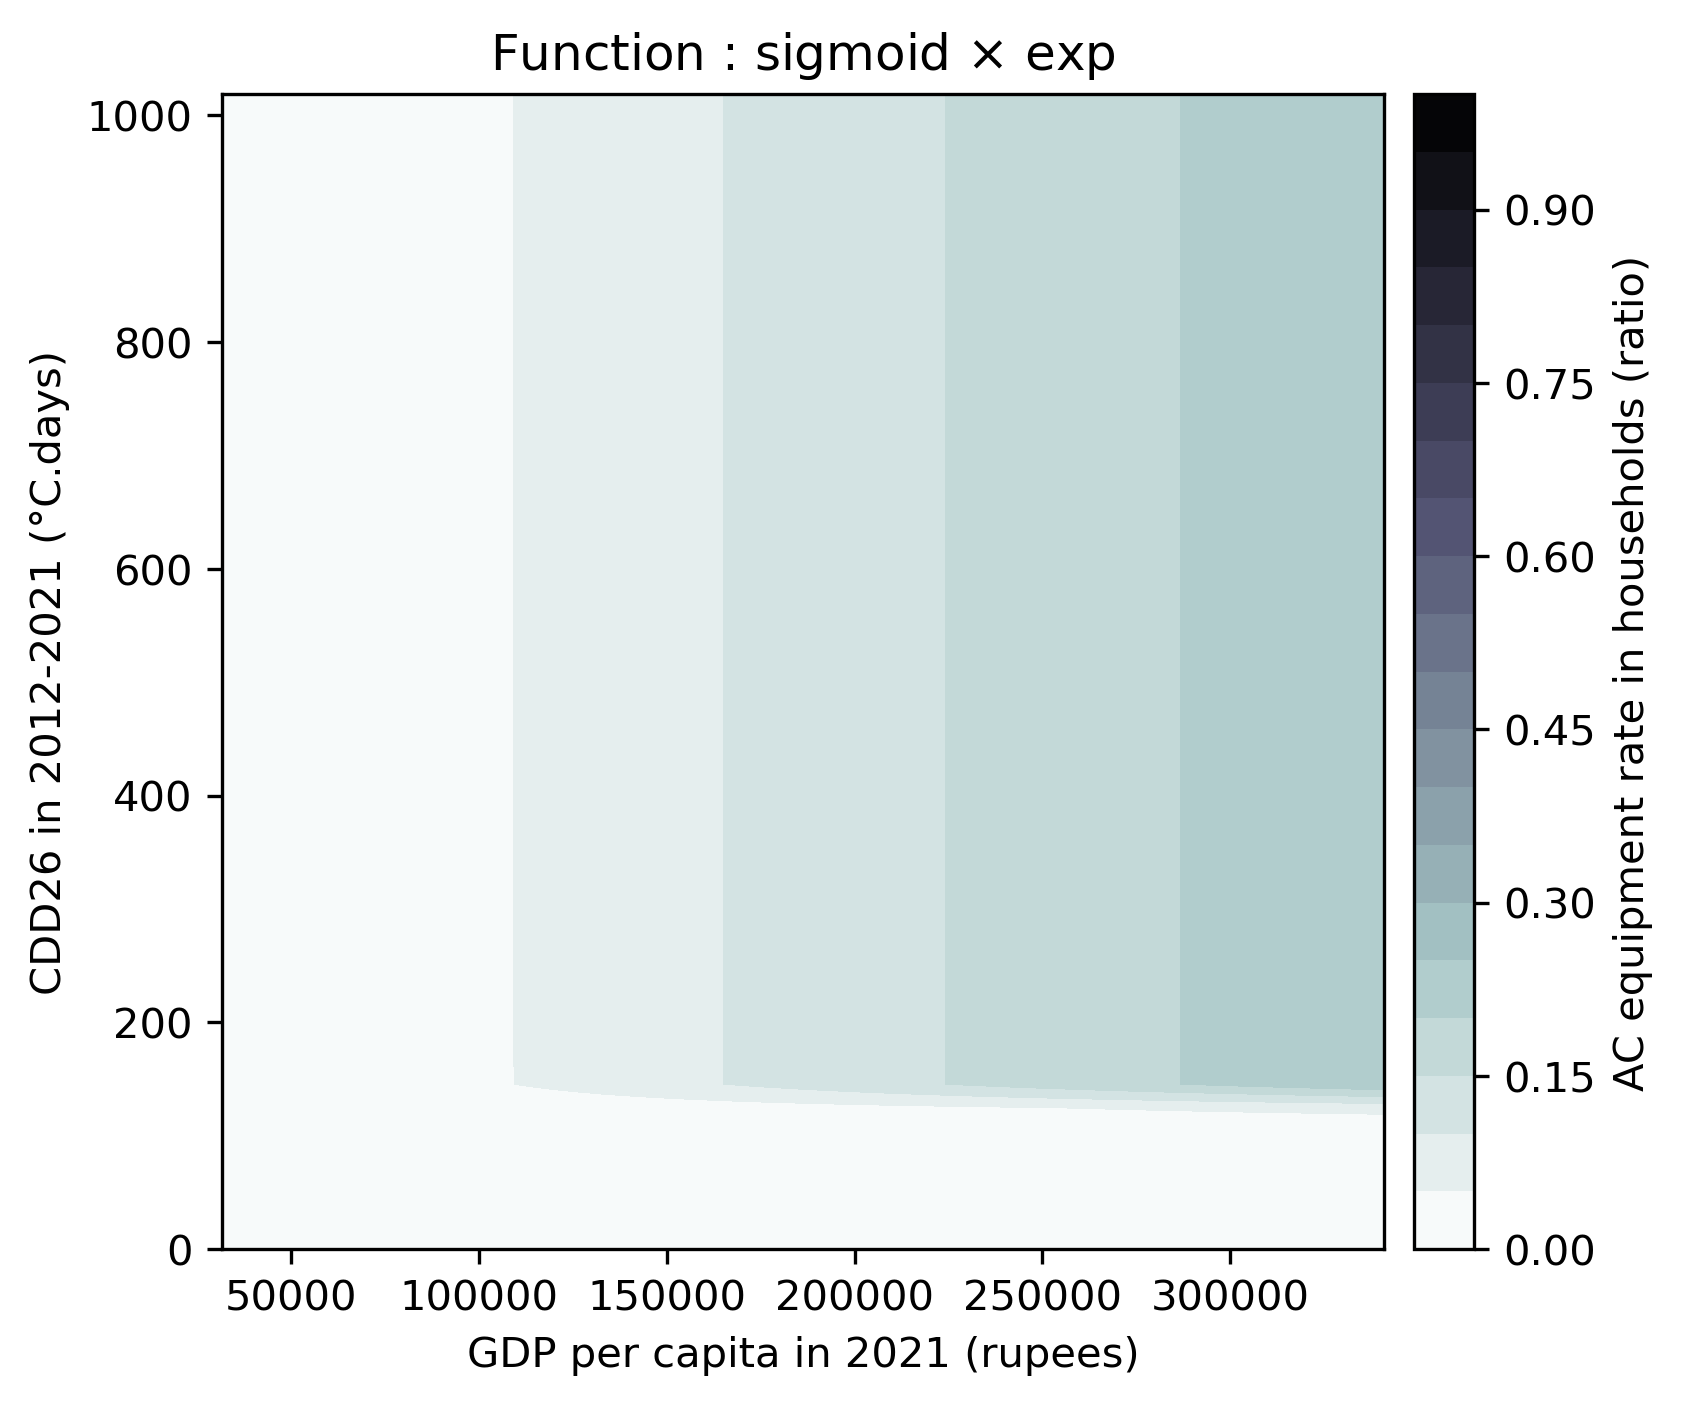
\includegraphics[width=0.38\columnwidth]{figures/cdd26_sigmoid_exp_2dplot.png}
   \caption{\label{fig:se} Résultats de modélisation. De haut en bas, CDD à seuils de 18, 21, 23 et \SI{26}{\celsius}.}
\end{figure}


\clearpage 
\section{Climatisation et refroidisseurs d'air}

\subsection{Nombre de climatiseurs par foyers}

Dans les données d'enquête, on connaît le nombre de système de climatisation qu'ont les ménages dotés de la climatisation. Ces données sont décrites \ref{fig:nb_ac}.

\begin{figure}[ht]
   \centering
   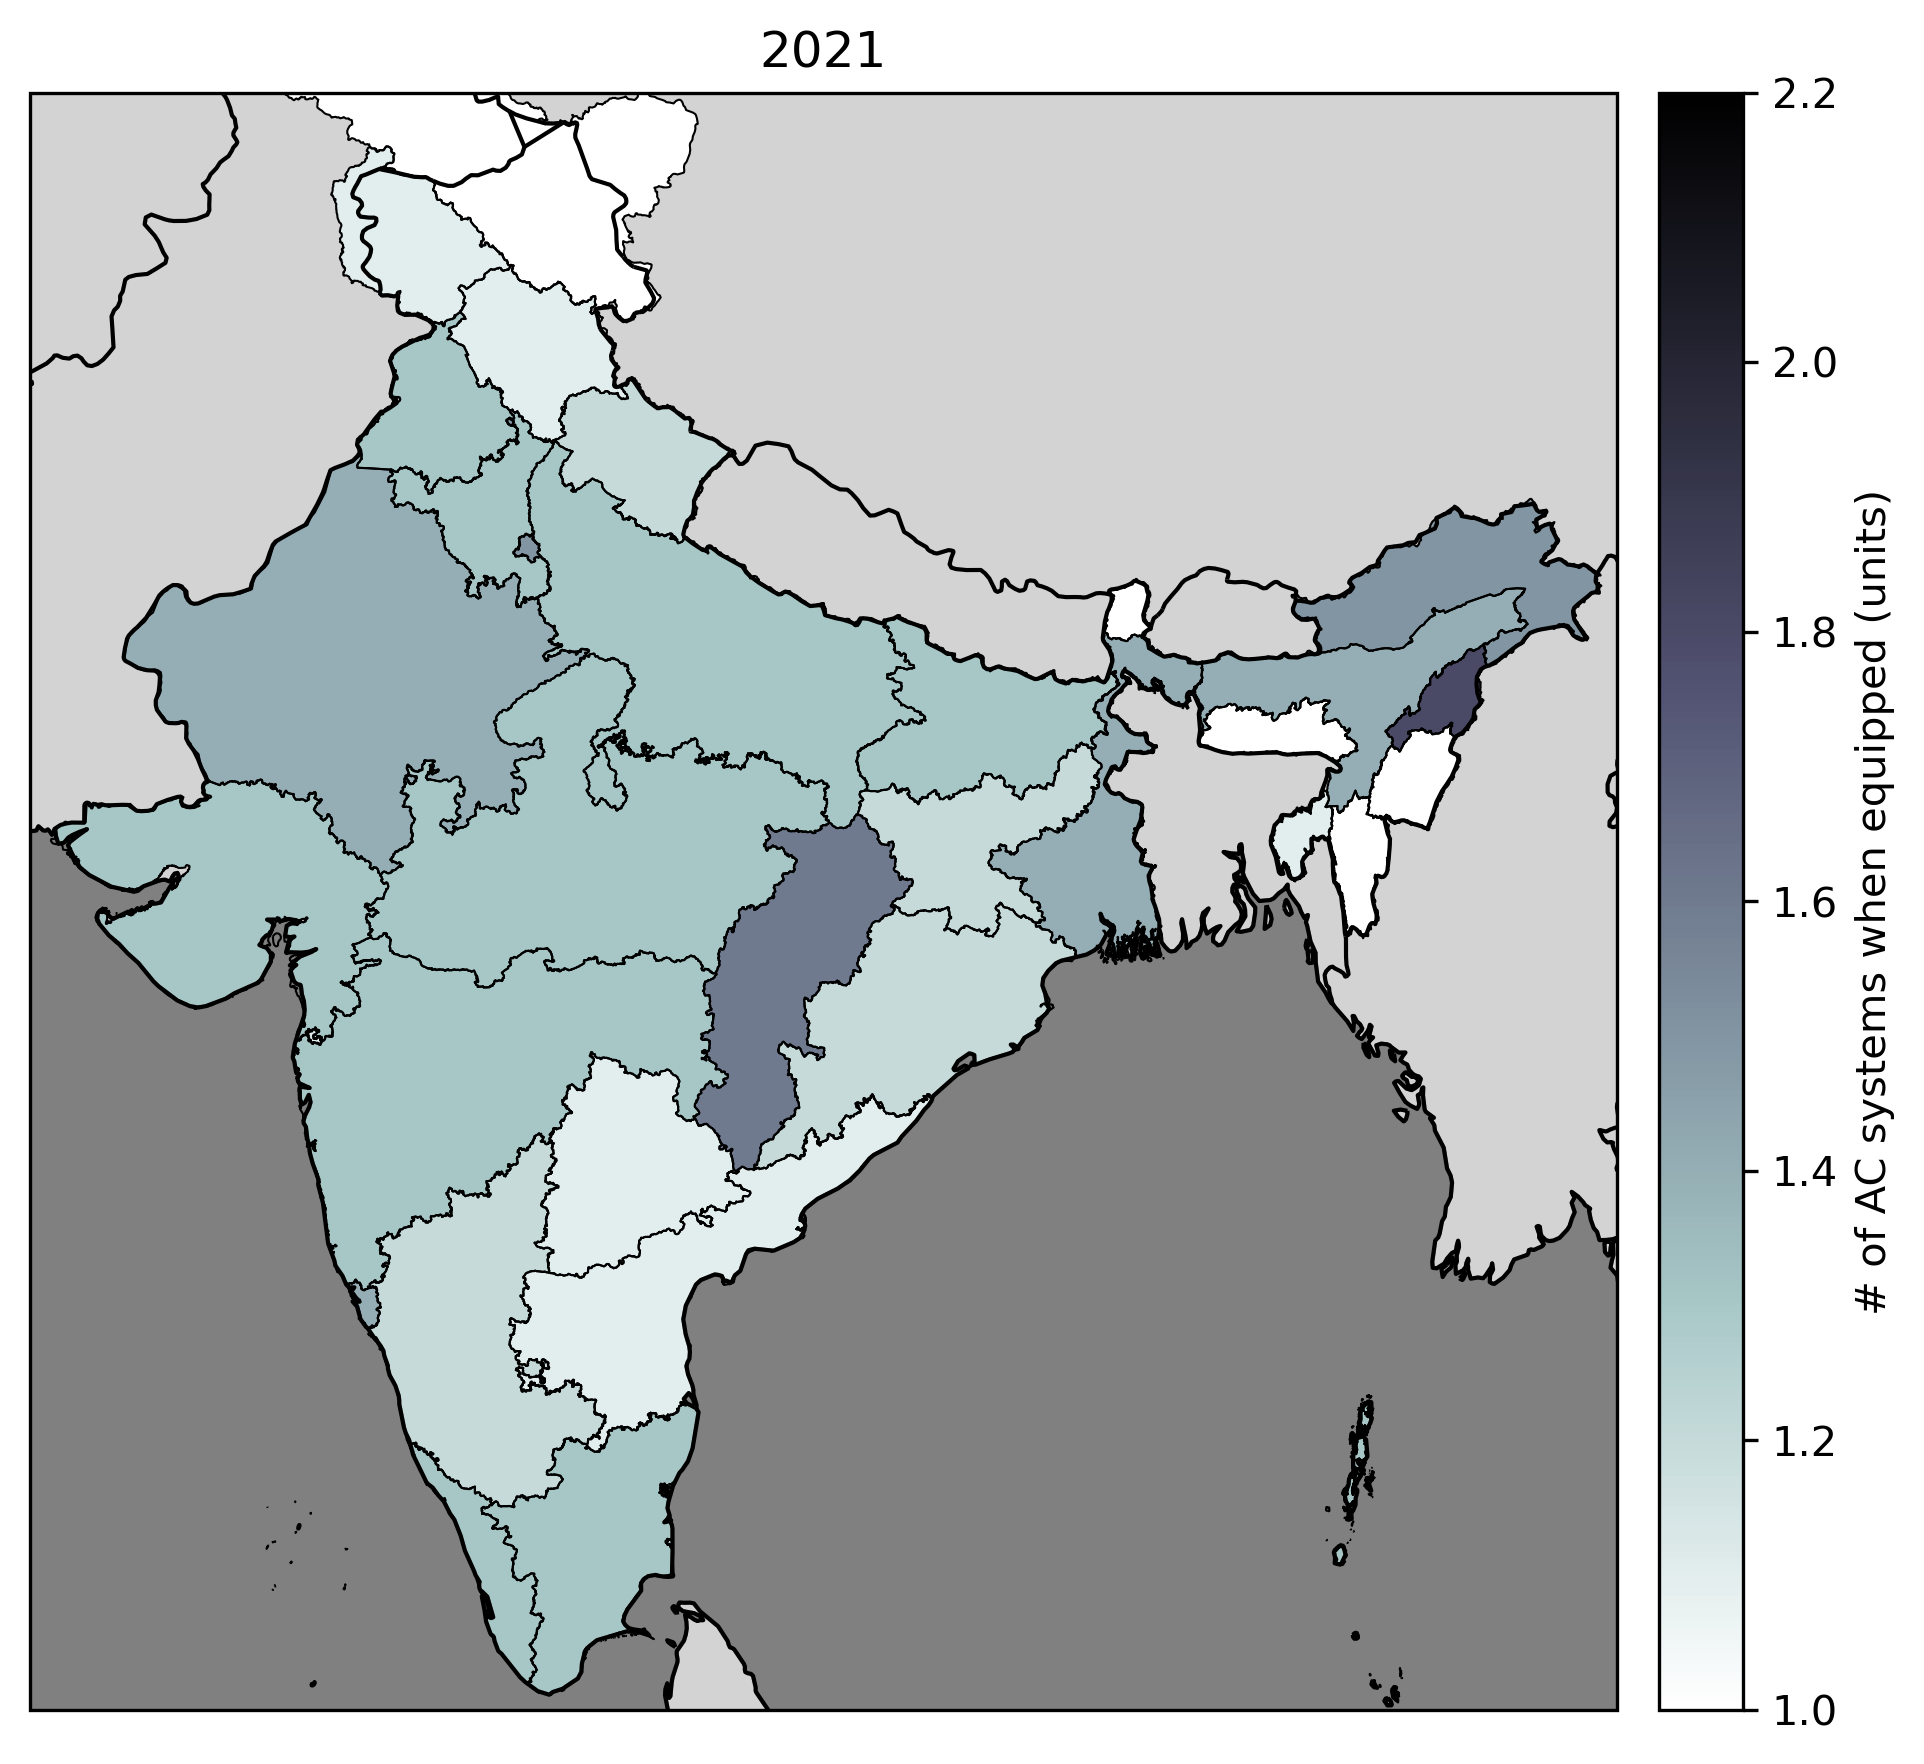
\includegraphics[width=0.36\columnwidth]{figures/20260404_nb_ac_when_ac_2021.png}
   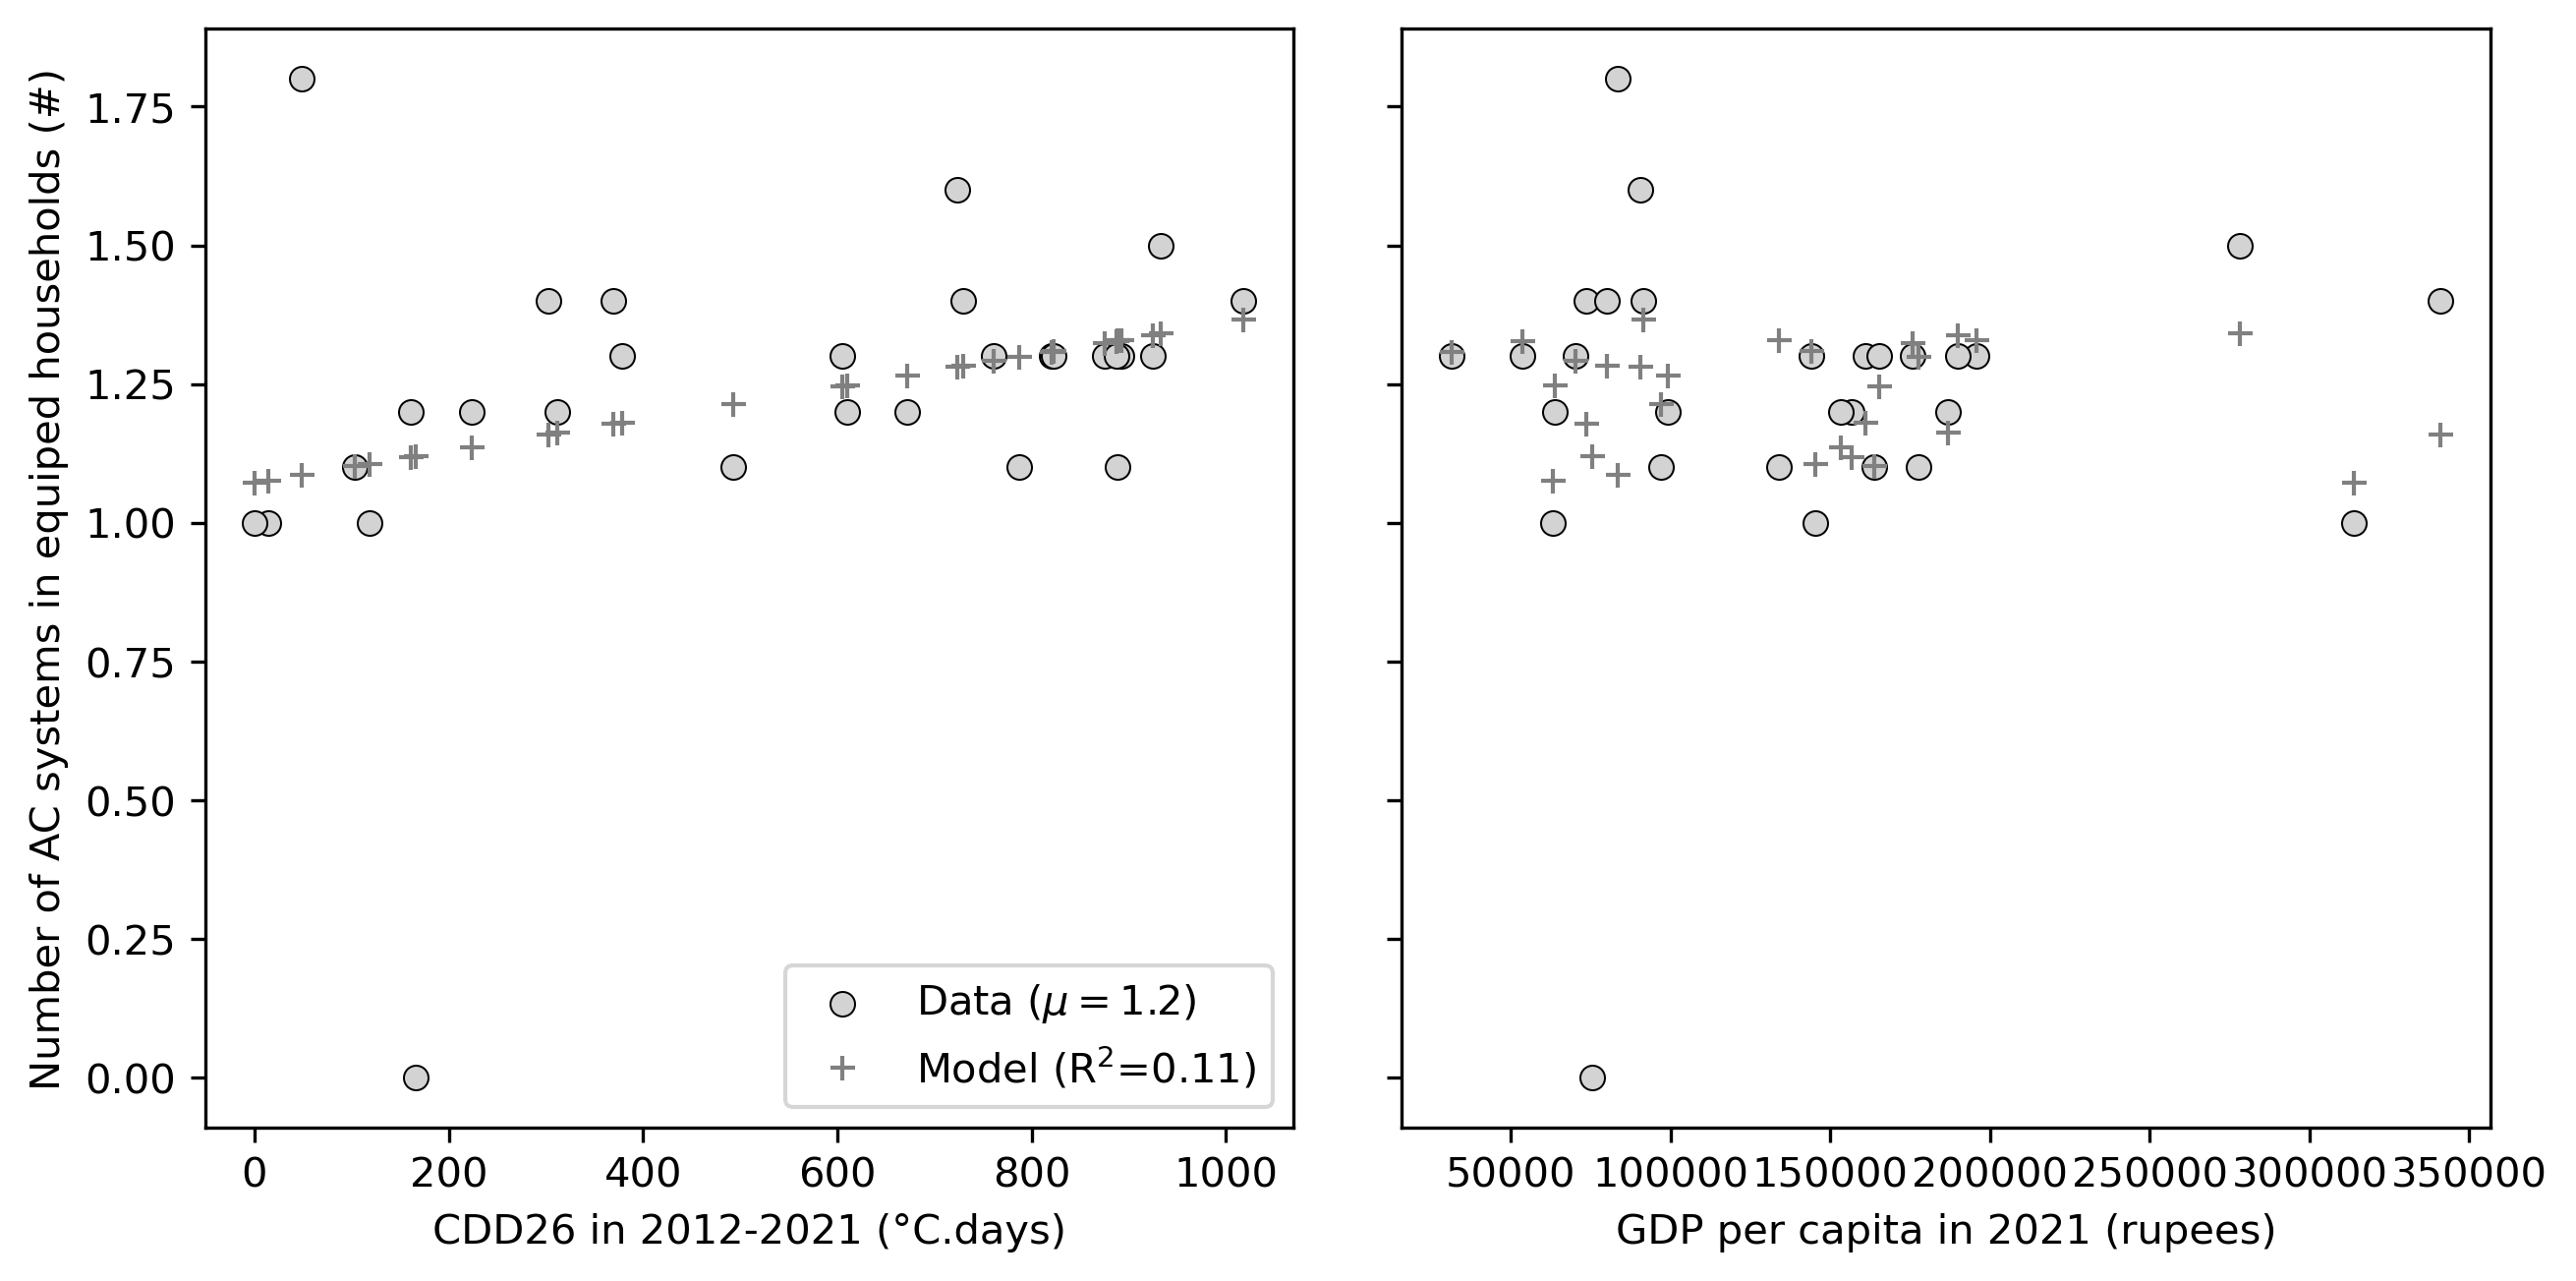
\includegraphics[width=0.63\columnwidth]{figures/cdd26_nb_ac_when_ac_scatter.png}
   
   \caption{\label{fig:nb_ac} Nombre de systèmes de climatisation par ménage équipé. }
\end{figure}

La valeur moyenne est de \num{1.2} systèmes par ménage équipé. De manière plus précise, on peut relier linéairement ce nombre ($N_\mathrm{AC}$) à la valeur de CDD26 \eqref{eq:nb_ac}
\begin{equation}
   \label{eq:nb_ac} 
   N_\mathrm{AC}(\mathrm{CDD}) = 1.07 + \num{2.88e-4}\cdot \mathrm{CDD}
\end{equation}


\subsection{Refroidisseurs d'air}

En plus des systèmes de climatisation, les enquêtes incluent des données sur les refroidisseurs d'air. Il s'agit de systèmes moins énergivores mais qui pourraient être inclus dans l'analyse car ceux-ci sont relativement présents dans les foyers indiens. De la même manière que la climatisation, mais de manière uni-variée, on peut relier le taux d'équipement en refroidisseur au CDD26 (\ref{fig:tau_cooler} et équation \eqref{eq:tau_cooler}) et le nombre de refroidisseur par ménage équipé au PIB par habitant (\ref{fig:nb_cooler} et équation \eqref{eq:n_cooler}). 

\begin{subequations}\label{eq:cooler}
     \begin{empheq}[left=\empheqlbrace]{align}
     \tau_\mathrm{cooler}(\mathrm{CDD}) &=  \frac{1}{1+\exp\left(-\alpha\cdot\left(\mathrm{CDD}-\beta\right)\right)} \quad\text{avec}\quad
     \begin{dcases}
        \alpha&= \SI{4.23e-03}{\per\degreeday}\\
        \beta &= \SI{1.14e+03}{\degreeday}
     \end{dcases}\label{eq:tau_cooler}\\
     N_\mathrm{cooler}(\mathrm{GDP}) &= 1+\exp\left(-\alpha\cdot\left(\mathrm{GDP}-\beta\right)\right) \quad\text{avec}\quad
     \begin{dcases}
        \alpha&= \text{\SI{8.51e-06}{\per\indianrupee}}\\
        \beta &= \text{\SI{-5.53e+04}{\indianrupee}}
     \end{dcases}\label{eq:n_cooler}
     \end{empheq}            
 \end{subequations}


 Le nombre de refroidisseur qui décroit avec le PIB moyen par habitant est difficilement interprétable. On pourrait penser que c'est lié au fait du choix de système de climatisation au détriment du refroidisseur mais le graphe présenté \ref{fig:ac_cooler} n'indique pas clairement cette relation. Les travaux de \textcite{pavanello_adapting_2024} pourraient permettre d'y voir plus clair. 

\begin{figure}[ht]
   \centering
   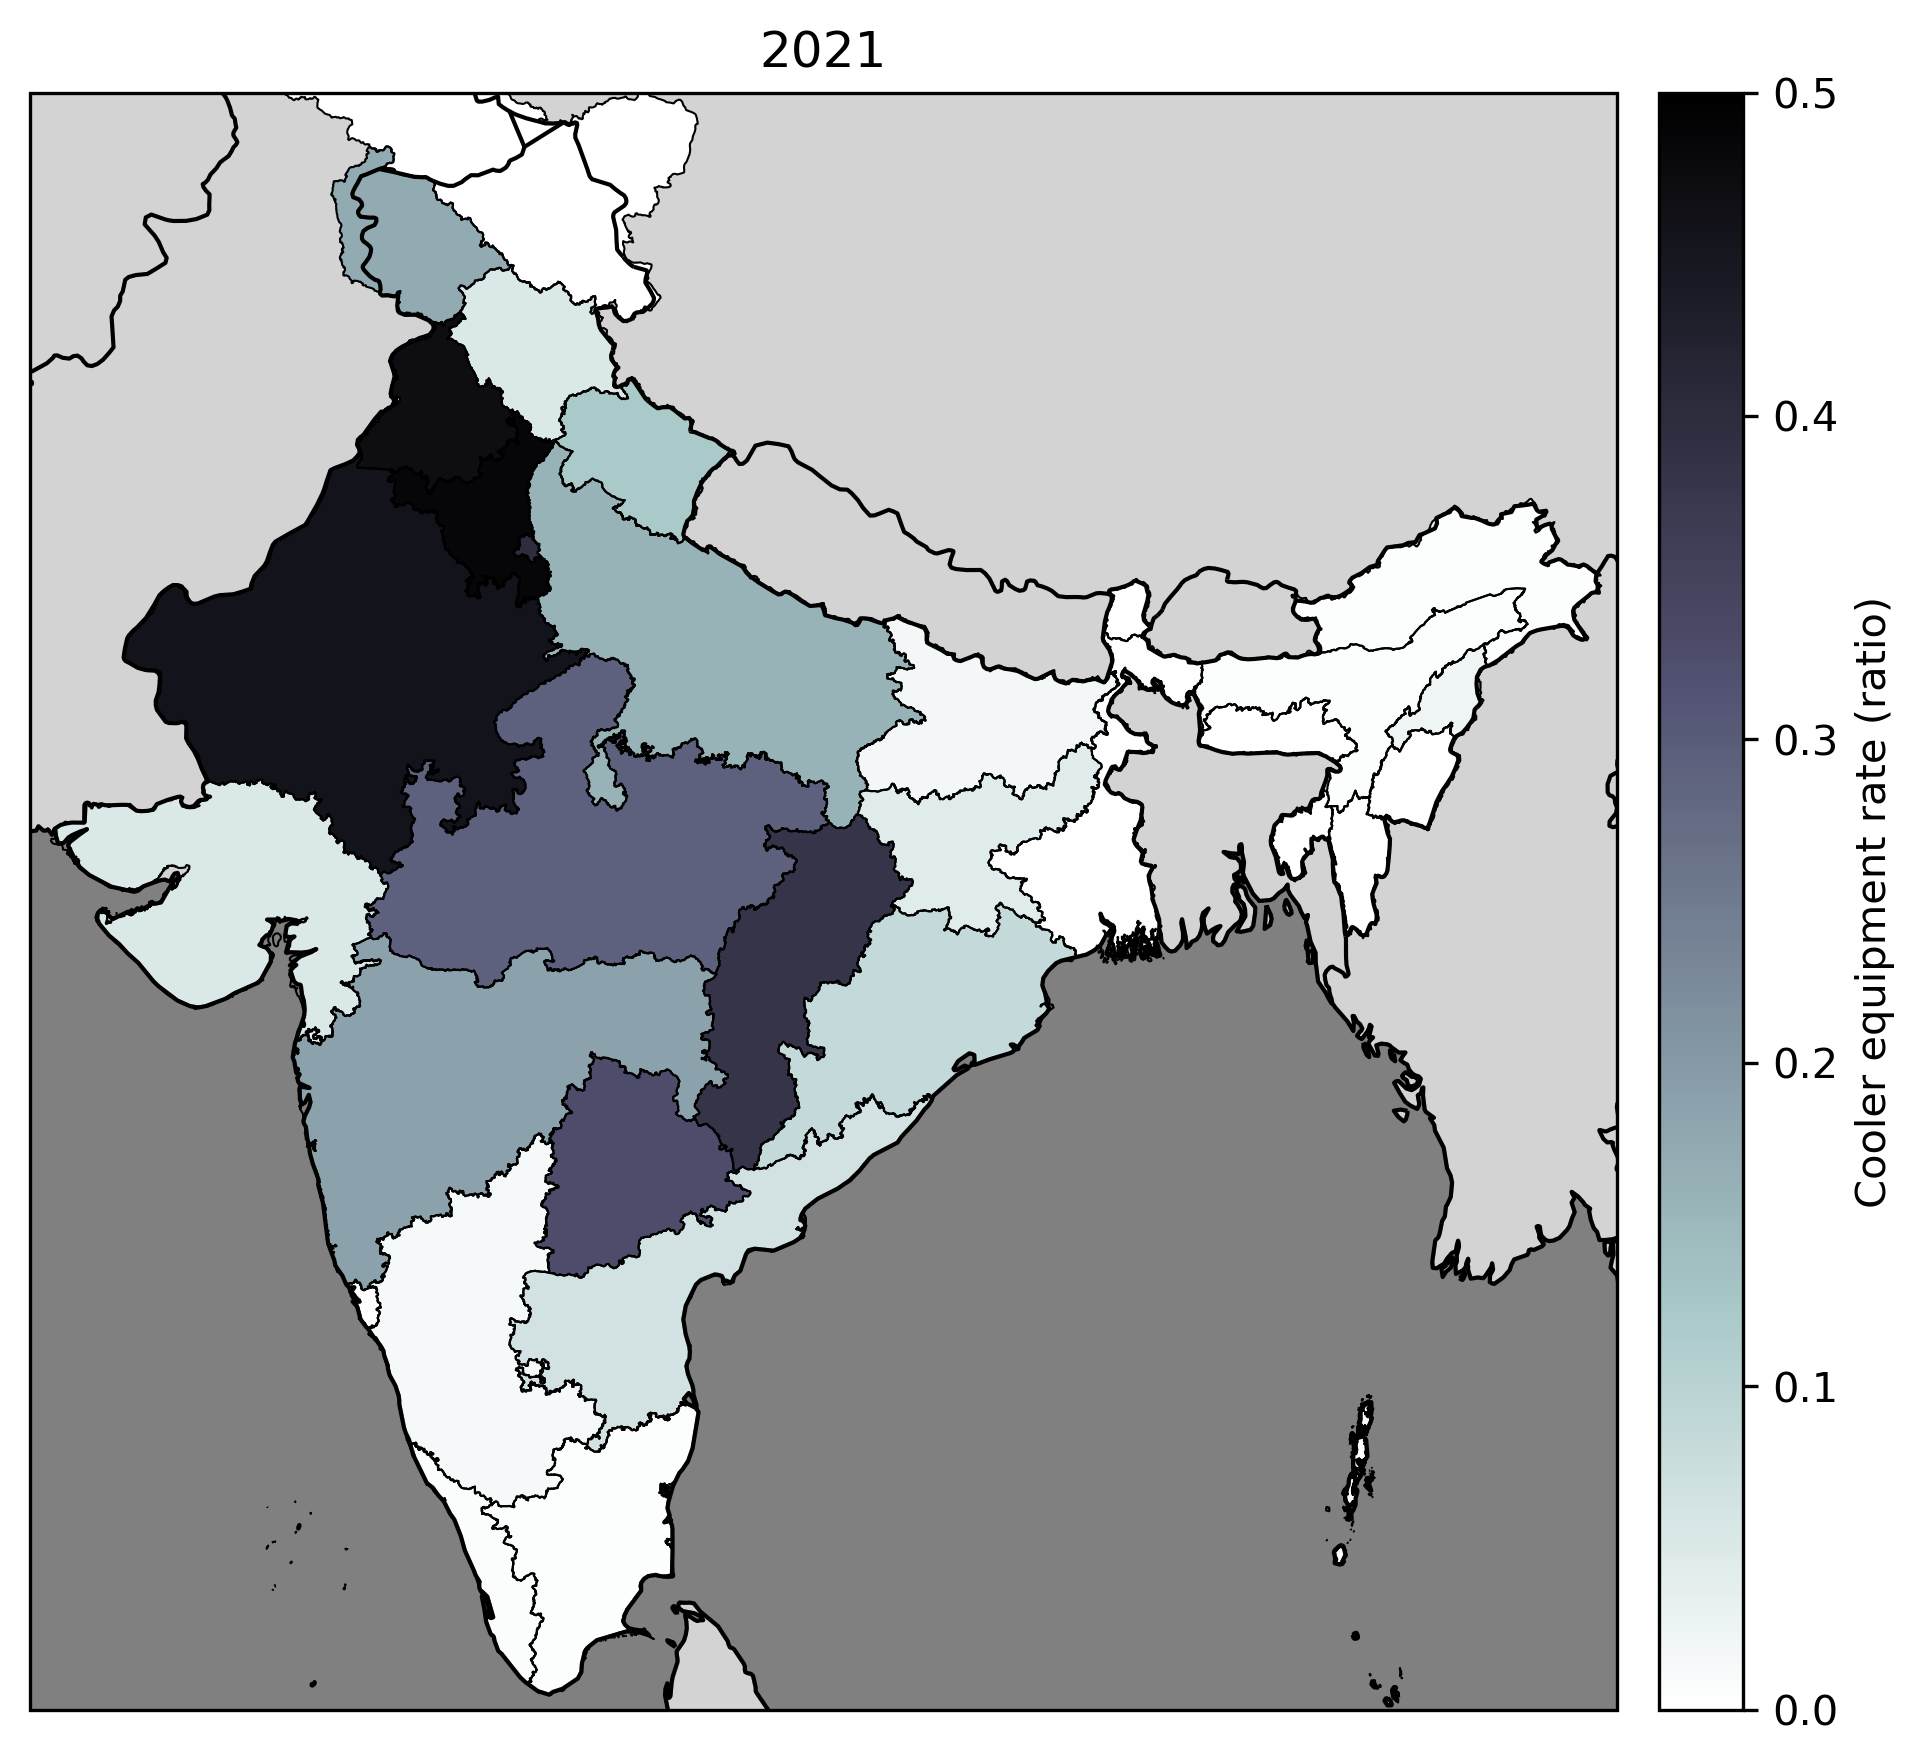
\includegraphics[width=0.36\columnwidth]{figures/20260404_cooler_rate_2021.png}
   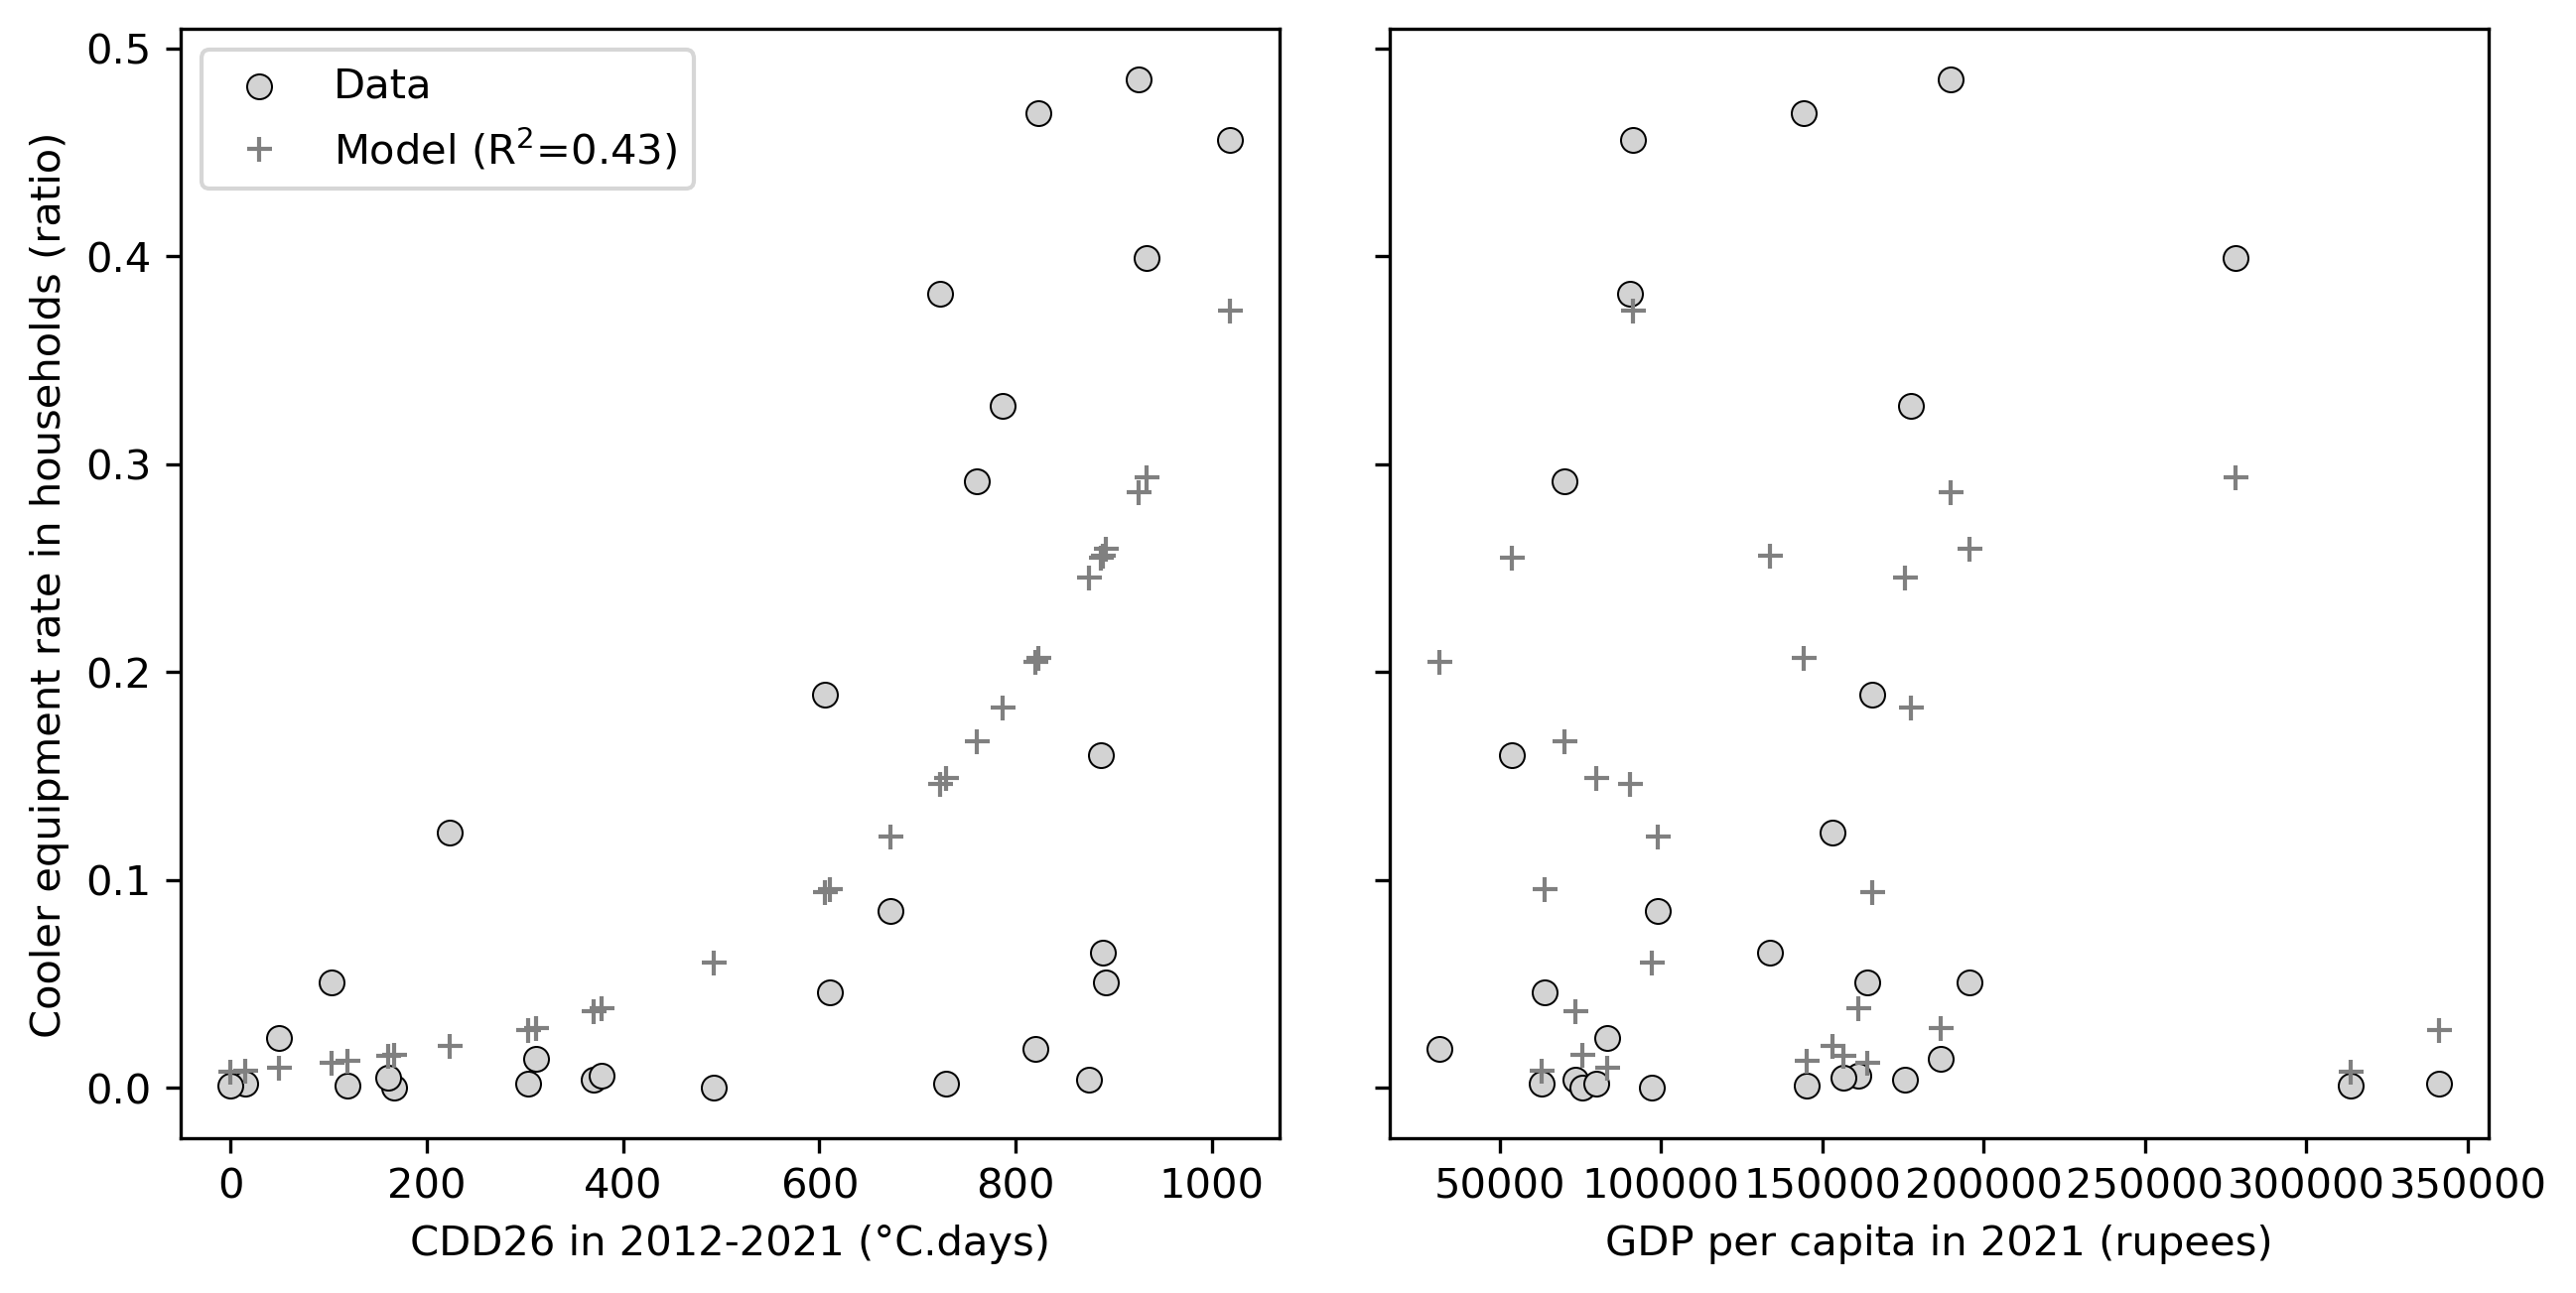
\includegraphics[width=0.63\columnwidth]{figures/cdd26_cooler_rate_scatter.png}
   
   \caption{\label{fig:tau_cooler} Taux d'équipement en refroidisseurs.}
\end{figure}

\begin{figure}[ht]
   \centering
   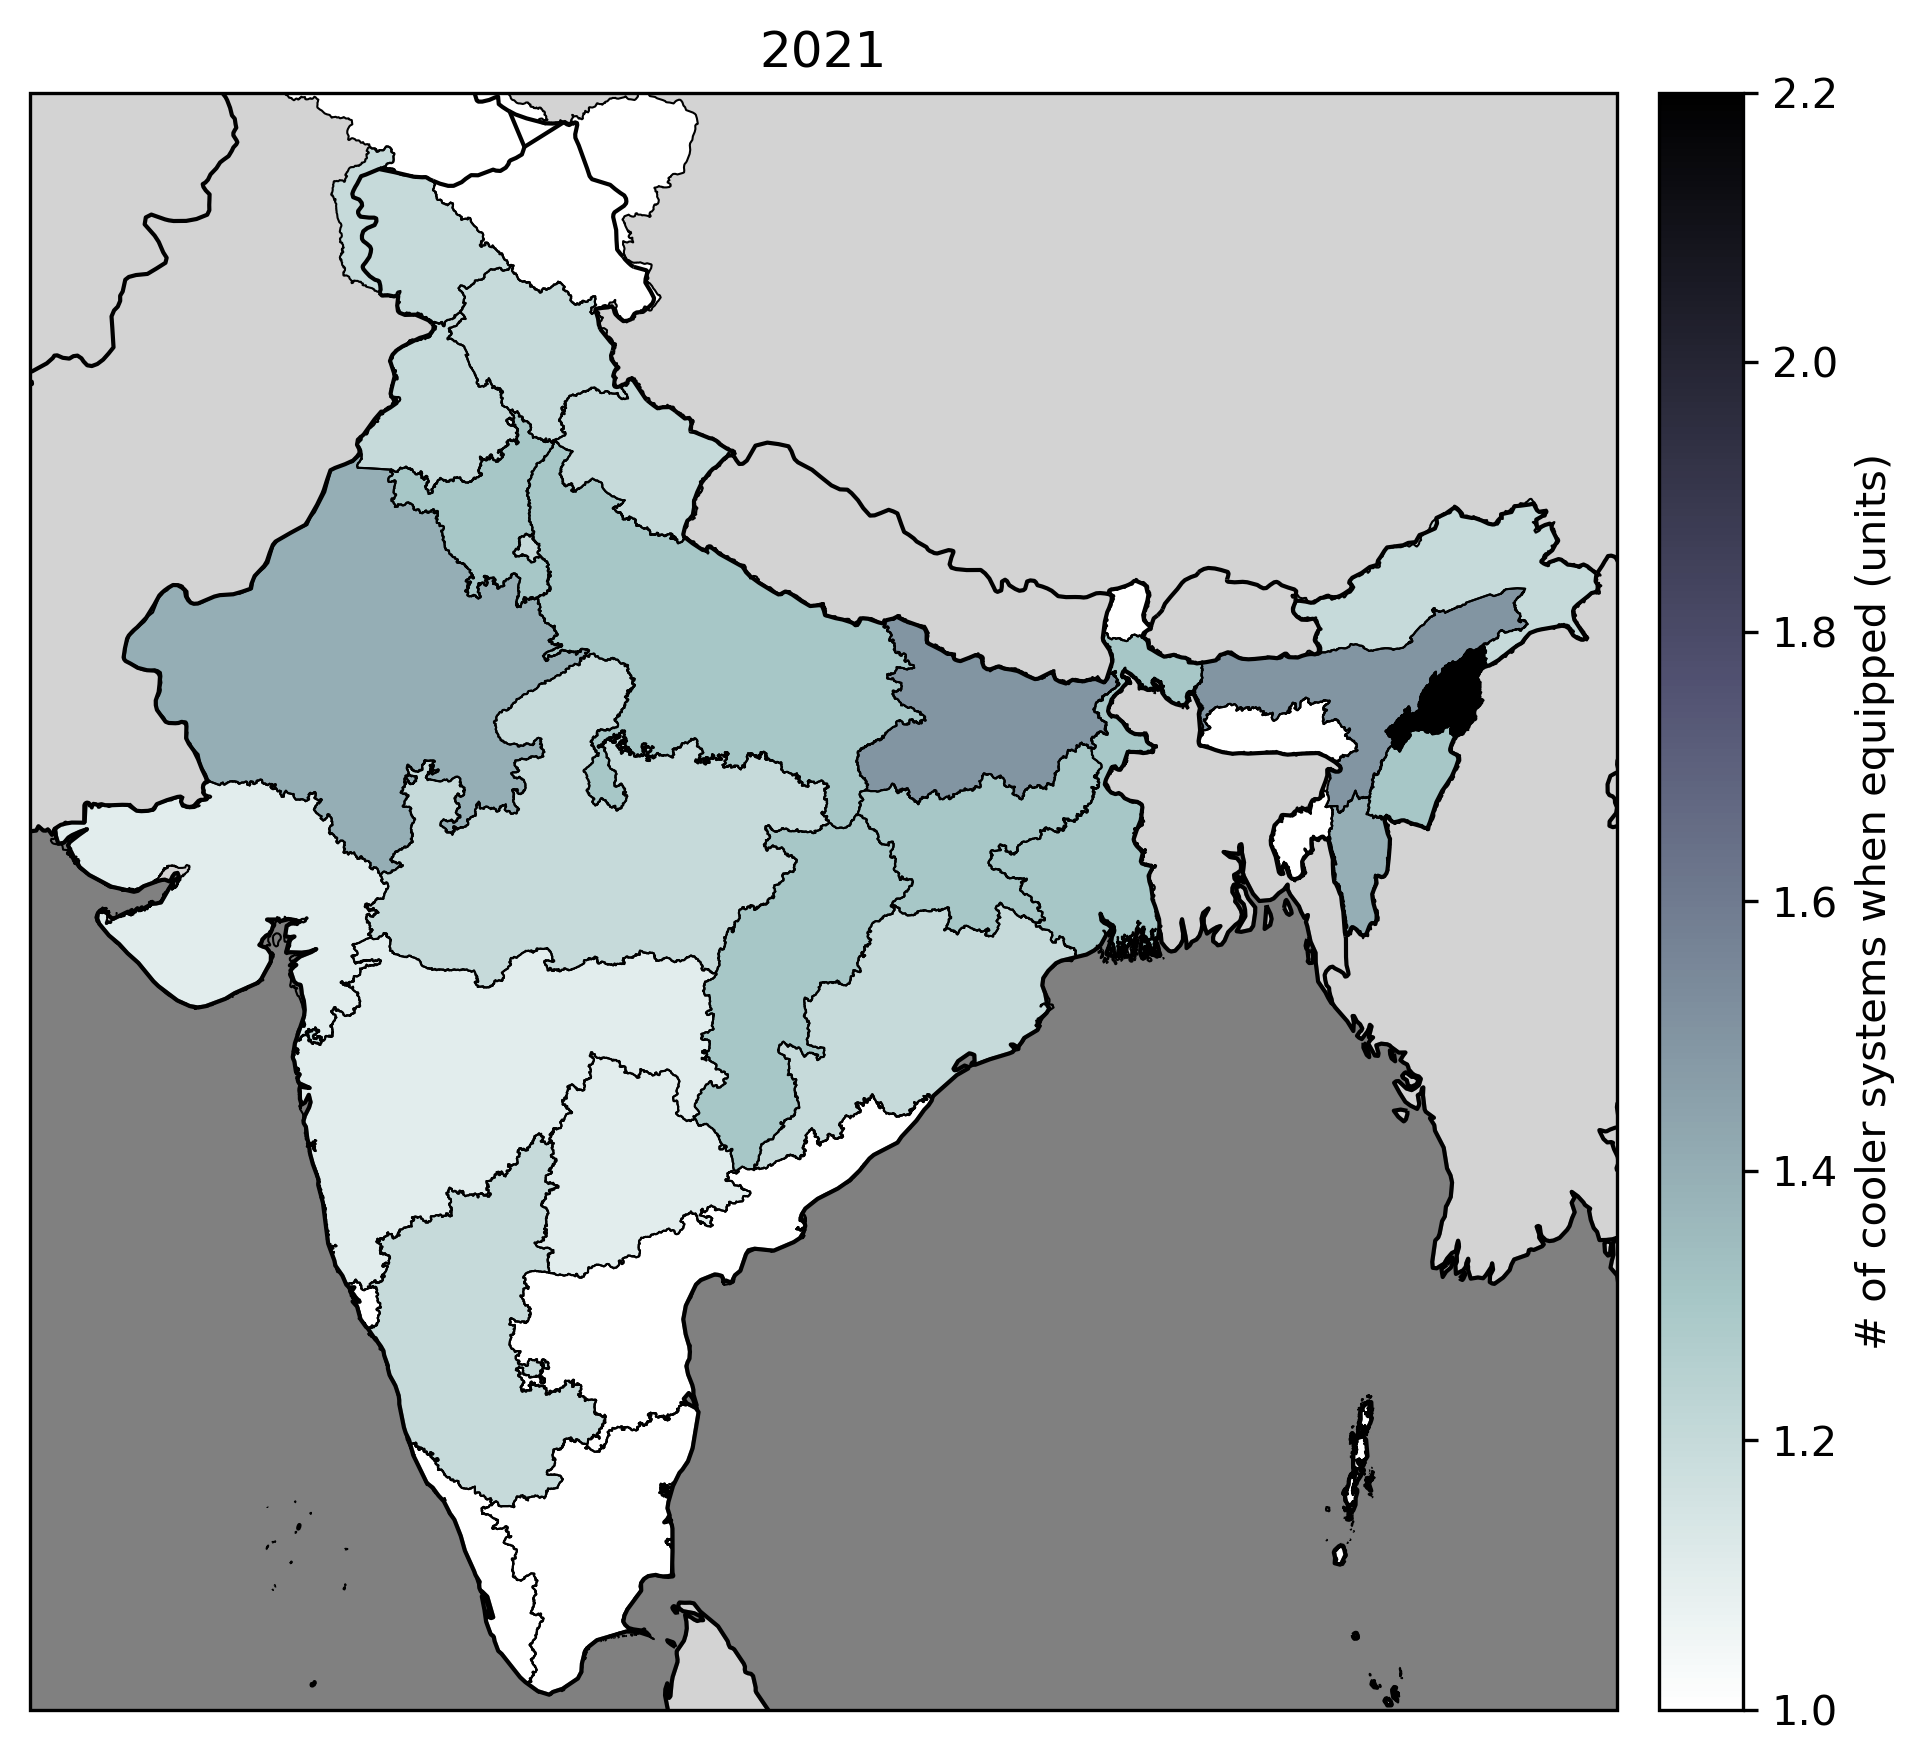
\includegraphics[width=0.36\columnwidth]{figures/20260404_nb_cooler_when_cooler_2021.png}
   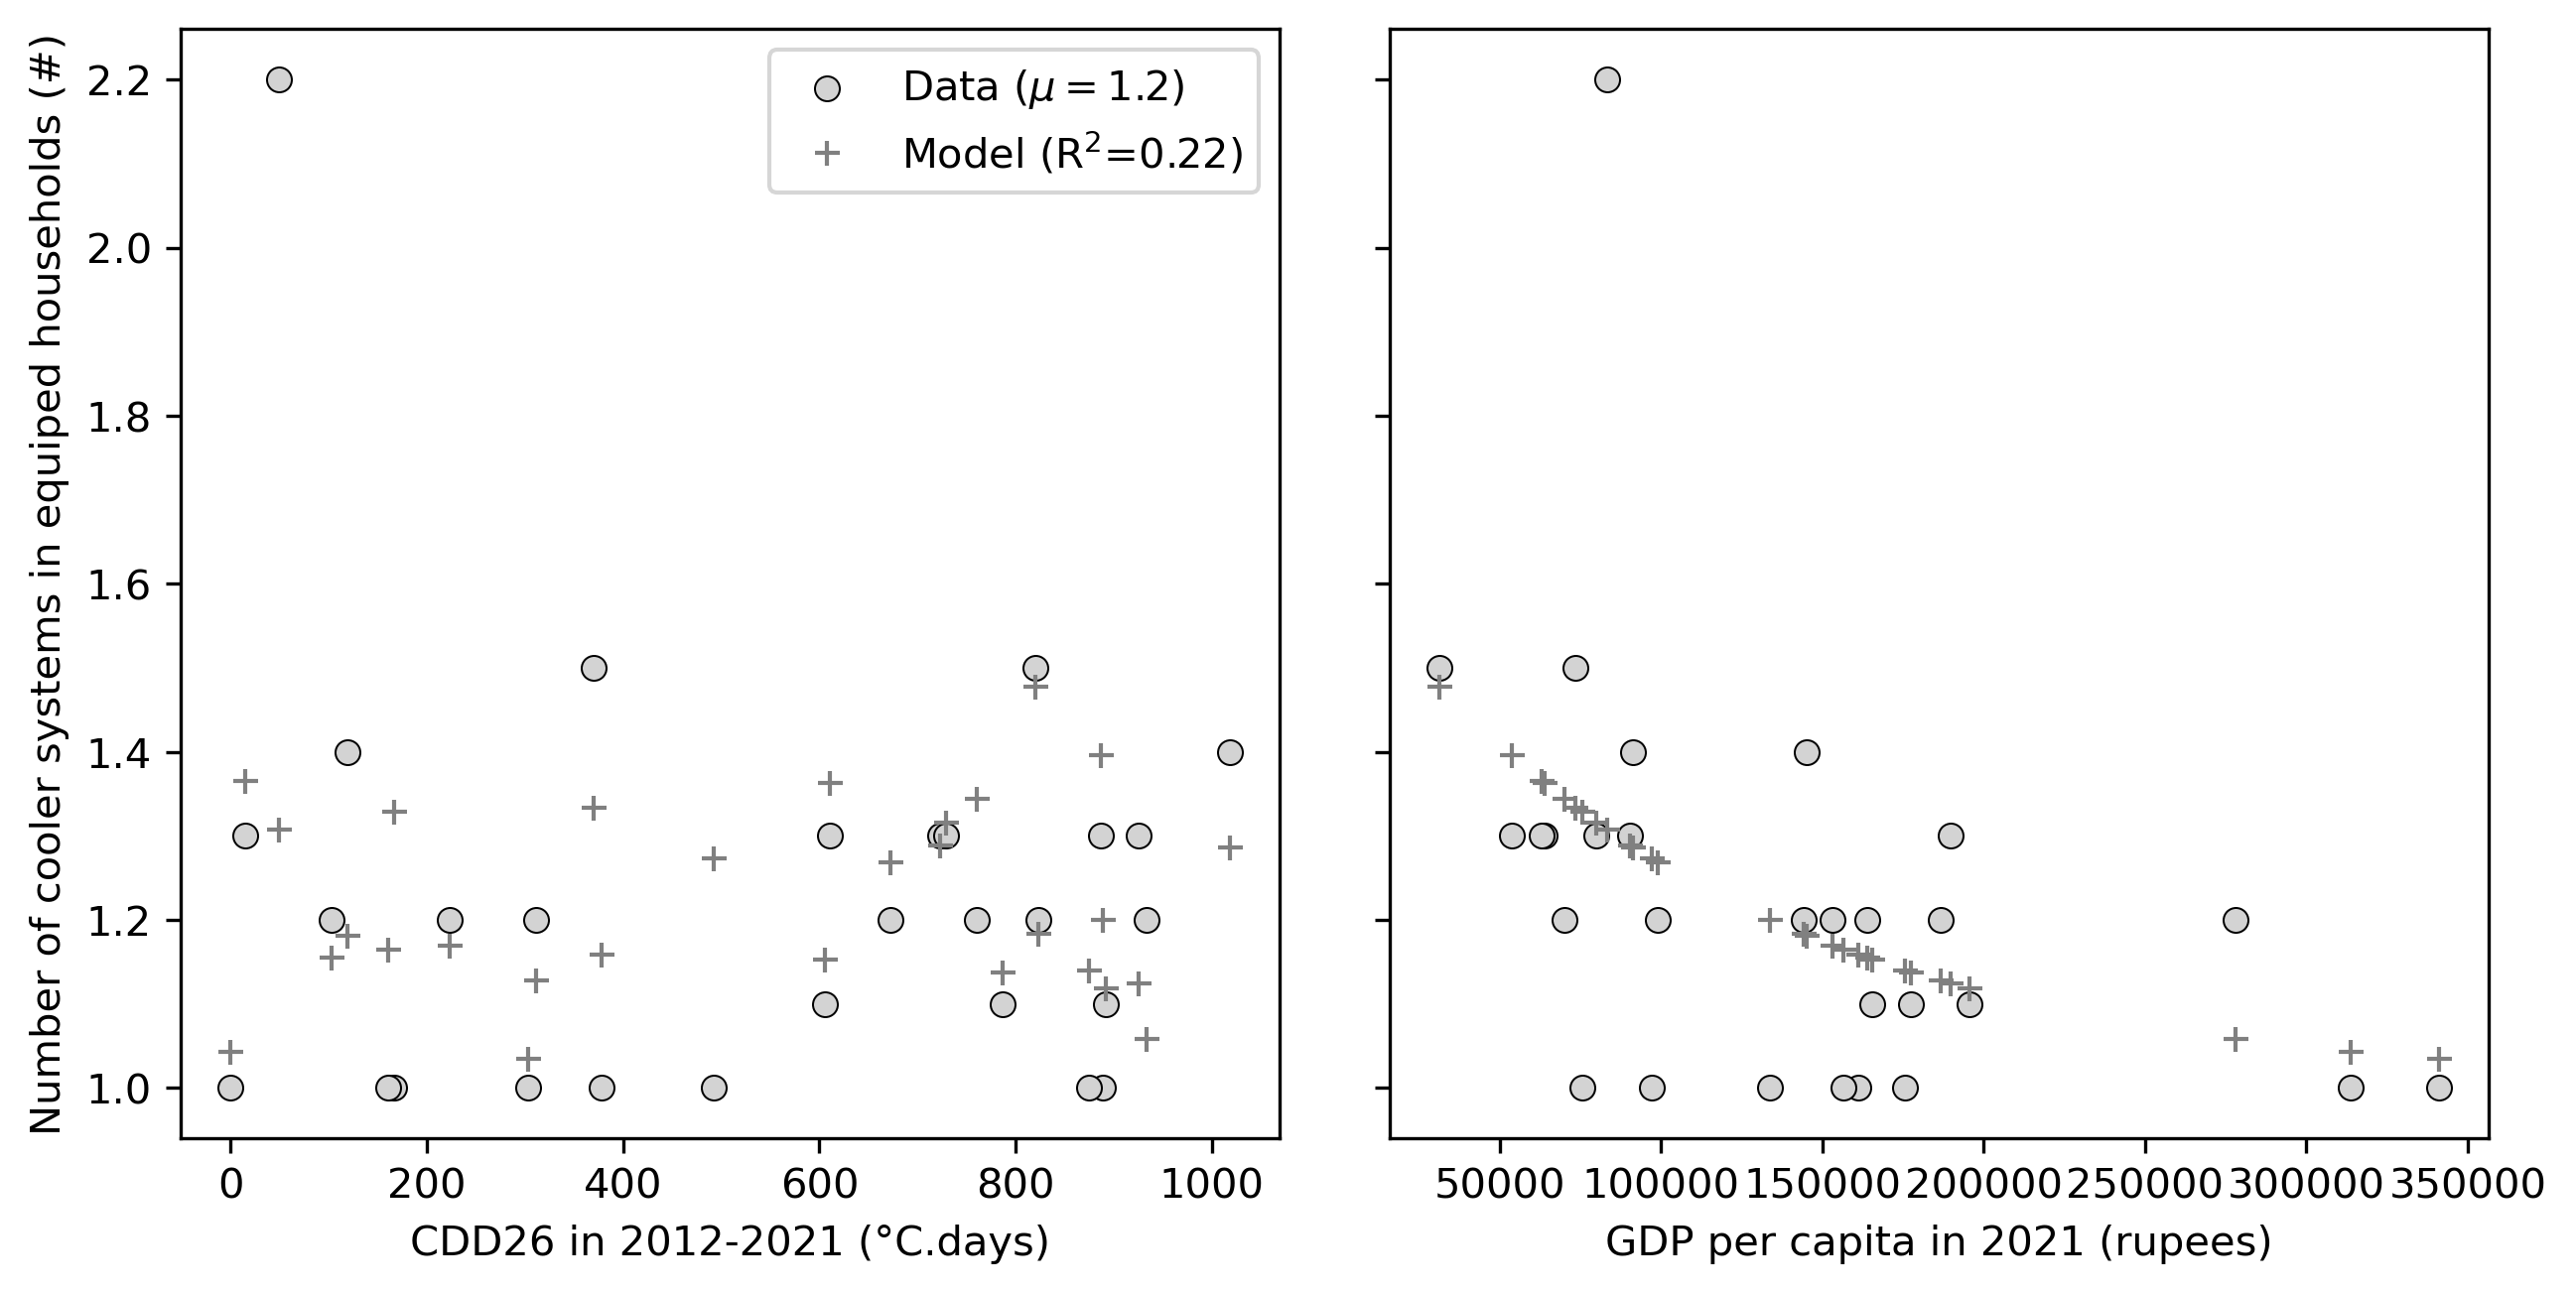
\includegraphics[width=0.63\columnwidth]{figures/cdd26_nb_cooler_when_cooler_scatter.png}
   
   \caption{\label{fig:nb_cooler} Nombre de refroidisseurs par ménage équipé. }
\end{figure}

\begin{figure}[ht]
   \centering
   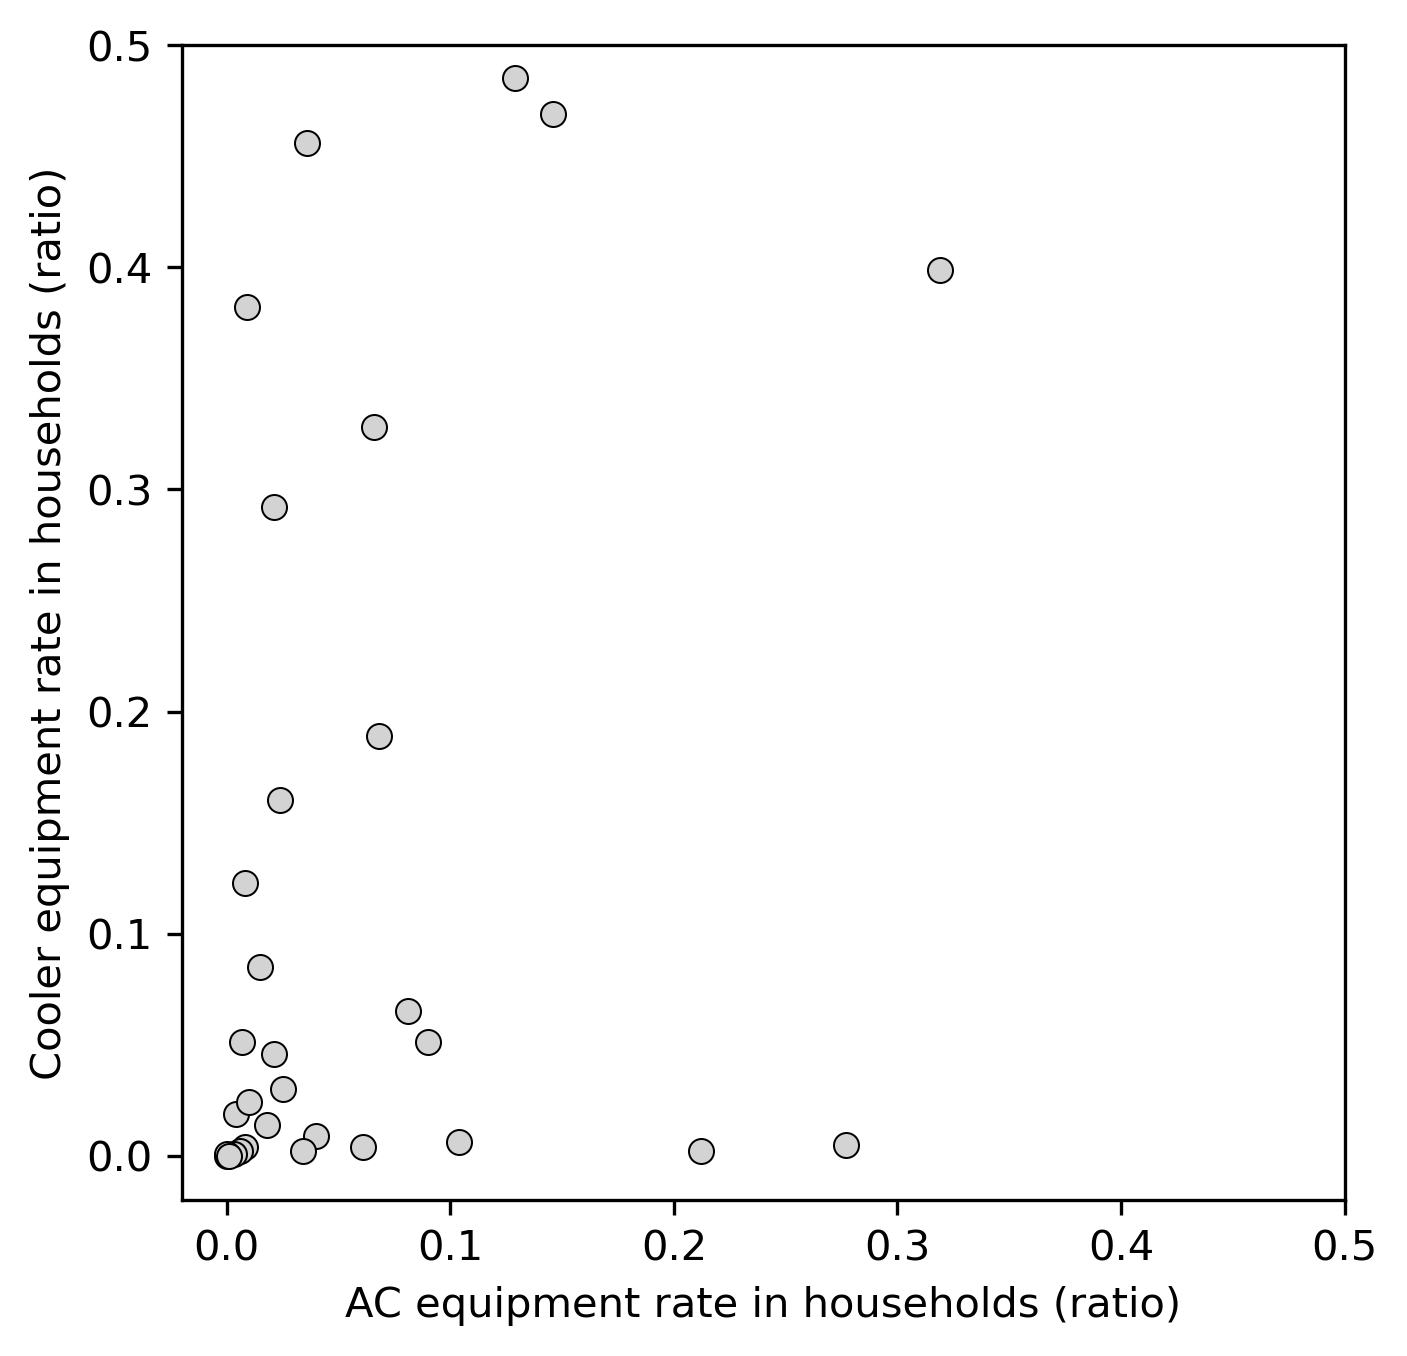
\includegraphics[width=0.4\columnwidth]{figures/cooler_ac_scatter_2021.png}
   
   \caption{\label{fig:ac_cooler} Taux d'équipement en refroidisseur par rapport à celui en climatisation. }
\end{figure}

\section{Suites}

\noindent 
Les éléments décrits ici permettent de poursuivre l'analyse :
\begin{enumerate}
   \item Projections de taux d'équipement puis de nombre de systèmes en circulation, à partir de la projections des températures (et CDD) issues de scénarios RCP et de projections de PIB par habitant issues de scénarios SSP;
   \item Calcul des consommations d'énergie liées à la climatisation résidentielles à partir de diverses hypothèses issues de différents articles (\cite{harish_impact_2020}, \cite{khosla_what_2021}, \cite{ramapragada_investigation_2022} et \cite{staffell_global_2023};
   \item Généraliser le développement et les consommations résidentielles à la climatisation tertiaire. 
\end{enumerate}

\clearpage
\printbibliography
\end{document}